\documentclass[11pt]{beamer}
\usepackage{graphicx}
\usepackage[export]{adjustbox}  % max width/height in includegraphics
\usepackage{xcolor}
\usepackage{ifthen}
\usepackage{fontspec}
\usepackage{textcomp}
% \usepackage[T1]{fontenc}
\usepackage{caption}


\usetheme[hideothersubsections]{Goettingen}
\usecolortheme{seahorse}
%%% \usetheme{Montpellier}
%%% \usecolortheme{dolphin}
\setbeamercovered{invisible}
\setbeamertemplate{navigation symbols}{\insertslidenavigationsymbol}
\setbeamertemplate{page number in head/foot}{}
\setbeamertemplate{blocks}[rounded][shadow=false]
% \setbeamerfont{section in sidebar}{size=\fontsize{4}{3}\selectfont}
% \setbeamerfont{subsection in sidebar}{size=\fontsize{4}{3}\selectfont}
% \setbeamerfont{subsubsection in sidebar}{size=\fontsize{4}{2}\selectfont}

\usepackage{microtype}
% \DisableLigatures[f]{encoding = *, family = *}

% \usefonttheme{professionalfonts} % using non standard fonts for beamer
\usepackage{tgheros}
\usefonttheme{serif}
\usepackage{XCharter}

\AtBeginSection[]{
  \begin{frame}
    \vfill
    \centering
    \begin{beamercolorbox}[sep=8pt,center,shadow=true,rounded=true]{title}
    \usebeamerfont{title}\insertsectionhead\par%
    \ifthenelse{\equal{\thisSectionName}{Bonus}}{}{
        \usebeamerfont{subtitle}\thisSectionName\par%
    }
    \end{beamercolorbox}
    \begin{center}
    \ifthenelse{\equal{\thisSectionName}{Colleges and Universities}}{
        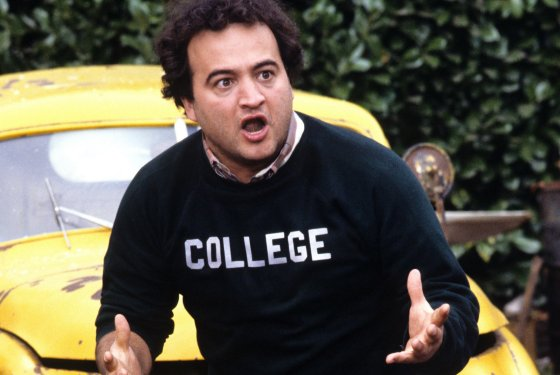
\includegraphics[max height = 0.3\textheight]{Images/belushicollege.jpg}
    }{}

    Please mute yourselves!
    \end{center}

    \ifthenelse{\equal{\thisSectionName}{Bonus}}
    {
        Get ready for some \emph{devilishly} hard questions!

        \vspace*{1em}
        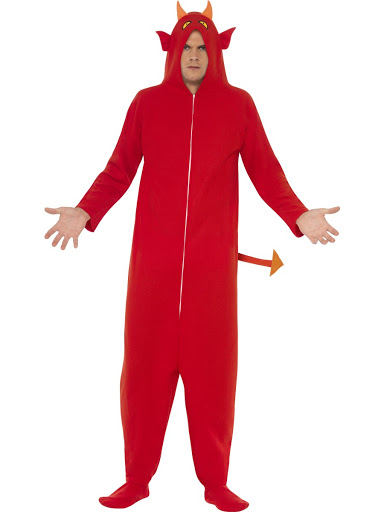
\includegraphics[max width=0.5\textwidth,
           max height=0.4\textheight]{Images/devil.jpg}
    }{}

    \vfill
  \end{frame}
}

\AtBeginSubsection[]{
  \begin{frame}
    \vfill
    \centering
    \begin{beamercolorbox}[sep=8pt,center,shadow=true,rounded=true]{title}
    \usebeamerfont{title}\insertsectionhead\par%
    \usebeamerfont{subtitle}\insertsubsectionhead\par%
    \end{beamercolorbox}
    \ifthenelse{\equal{\subsecname}{Answers}} {
        \begin{center}
        Unmute yourselves!
        \end{center}
    }
    \vfill
  \end{frame}
}
\begin{document}

\title{Welcome to Quarantine Trivia IX!\vspace{-0.5in}}
\date{}

\begin{frame}
\titlepage{}
\begin{center}
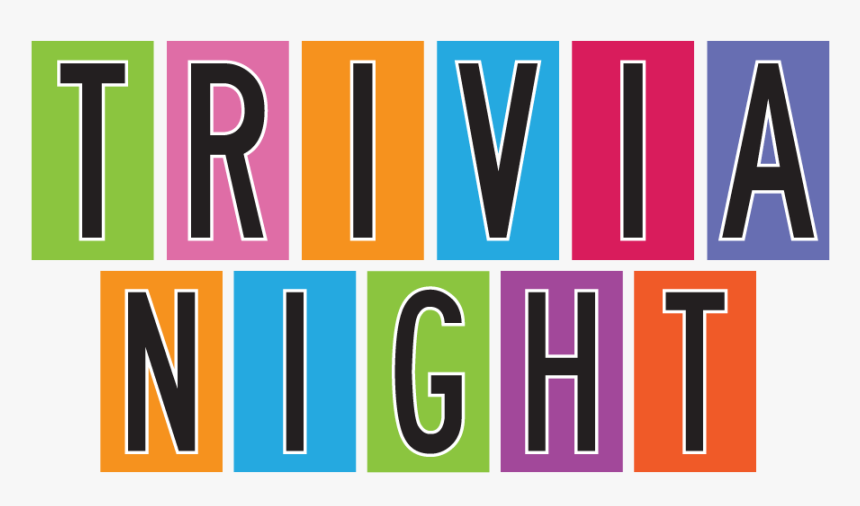
\includegraphics[max width=0.9\textwidth,
    max height=0.4\textheight]{Images/triviatitleframelogo.png}
\end{center}
\end{frame}

\begingroup{}
\begin{frame}[t]{}

It's been a pretty lousy week, but some good things did happen (and we're not being
ironic here):
\medskip{}

\only<2>{
    Jyoti Kumari, a fifteen year old girl who lives in India, rode her injured father
    700 miles from New Dehli back home on the back of her bicycle. This earned her the
    nickname ``Jyoti the Lionhearted''.
    \begin{center}
    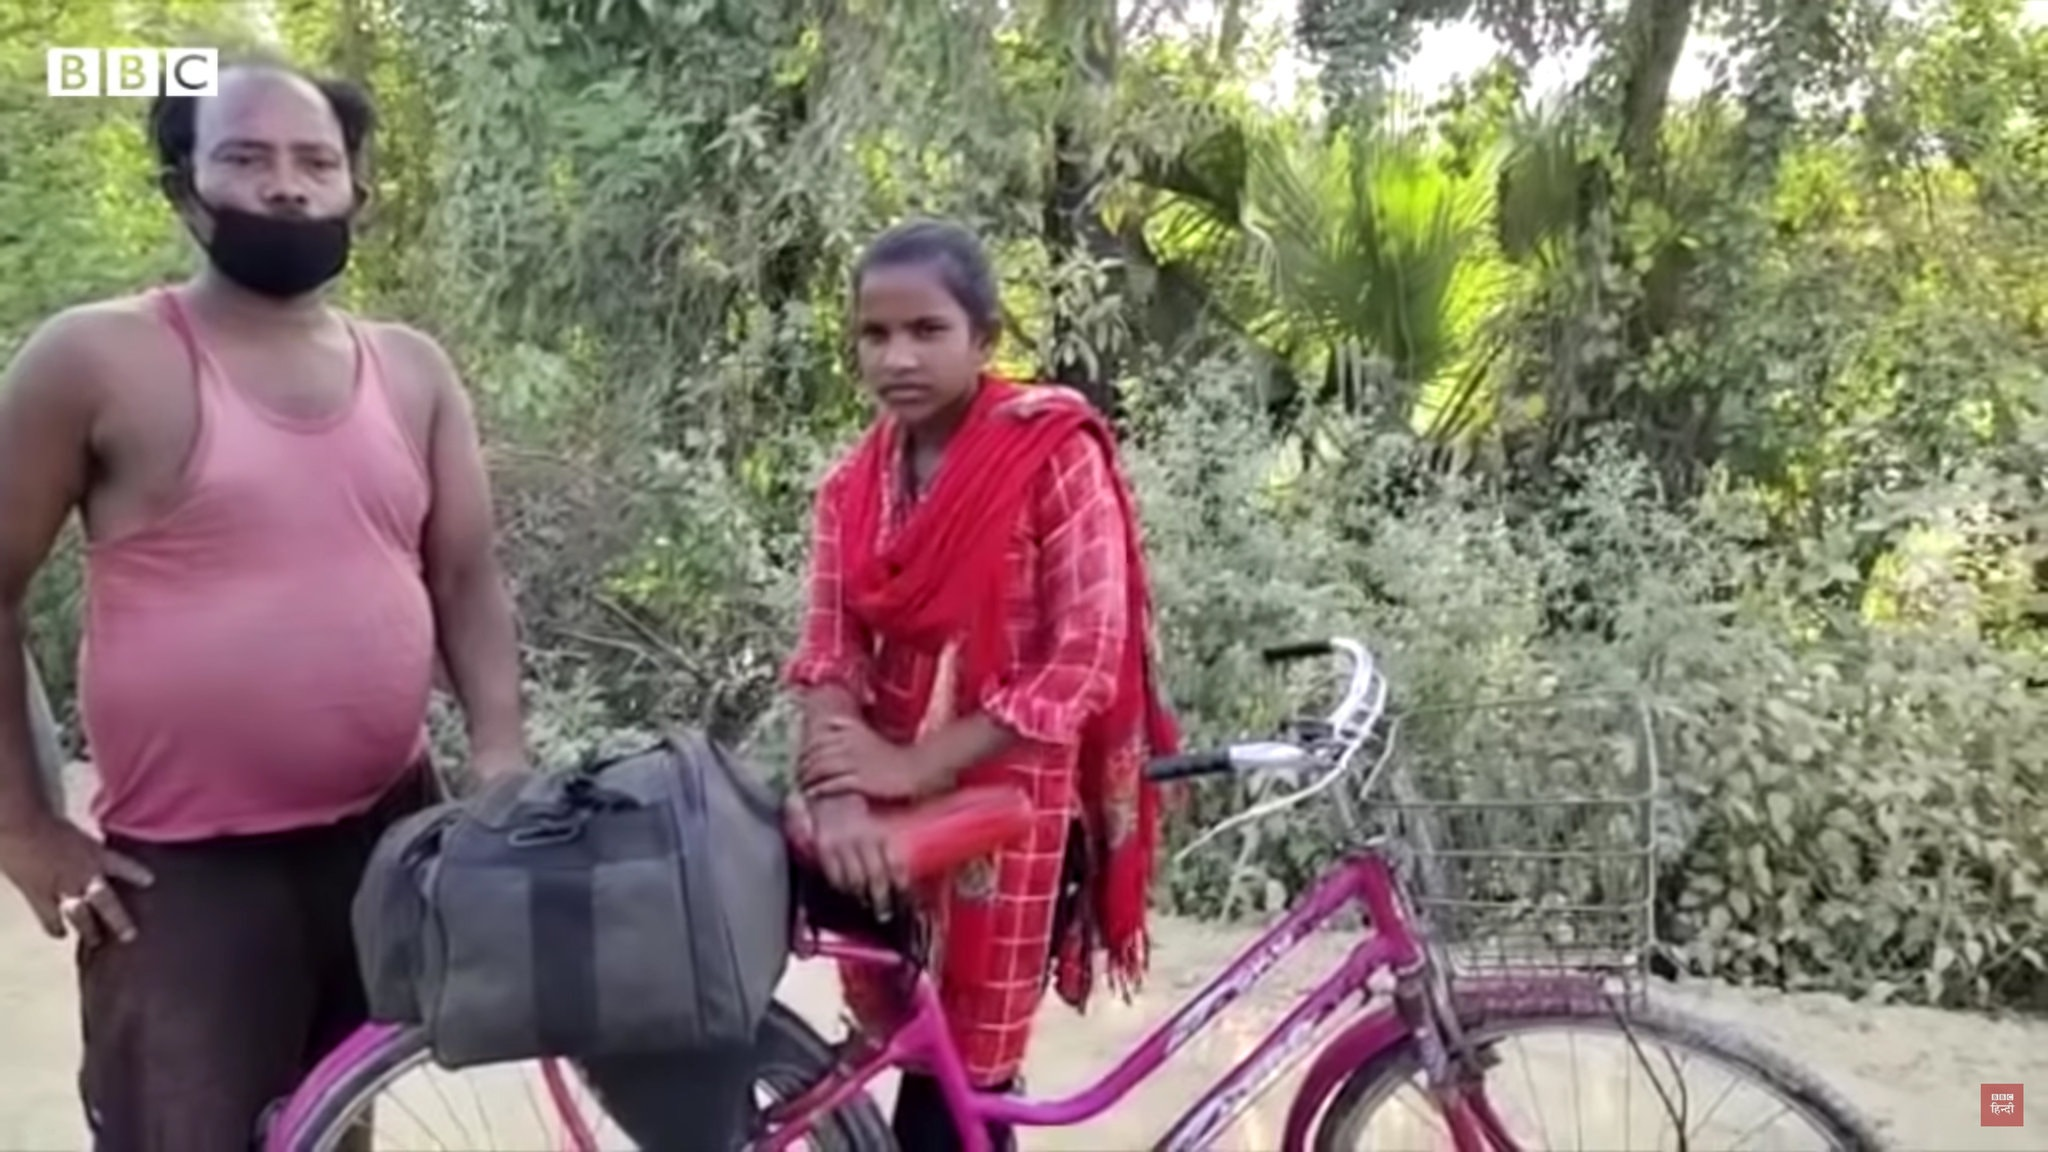
\includegraphics[max width=0.8\textwidth,max height=0.5\textheight]
    {{Images/jyoti}.jpg}
    \end{center}
}
\only<3>{
    British chef Ethan Rogers has created a six-foot-long ``Back to Work Baguette'',
    the sandwich for social distancers.
    \begin{center}
    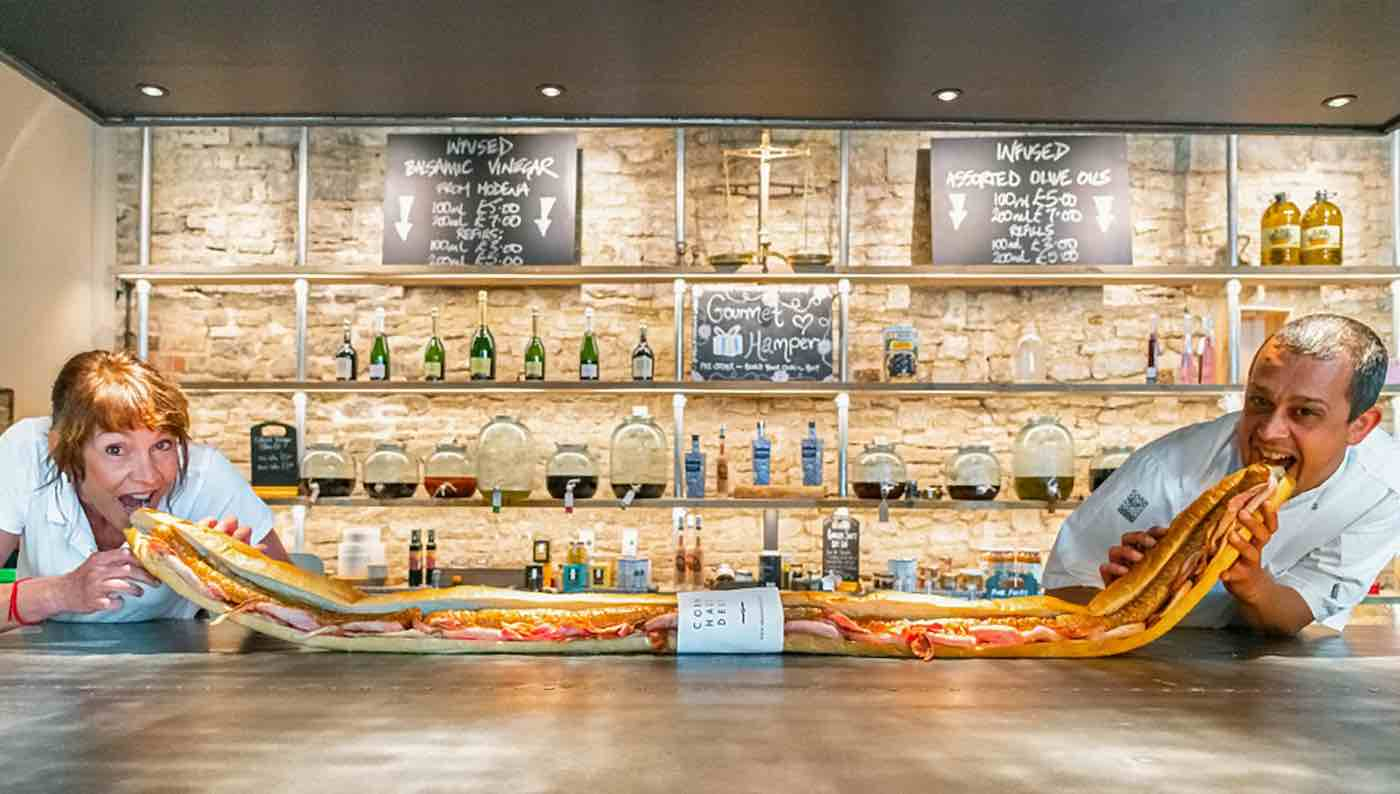
\includegraphics[max width=0.8\textwidth,max height=0.5\textheight]
    {{Images/sandwich}.jpg}
    \end{center}
}
\only<4>{
    With today's launch of SpaceX's Falcon 9, the U.S. resumed human spaceflight.
    \begin{center}
    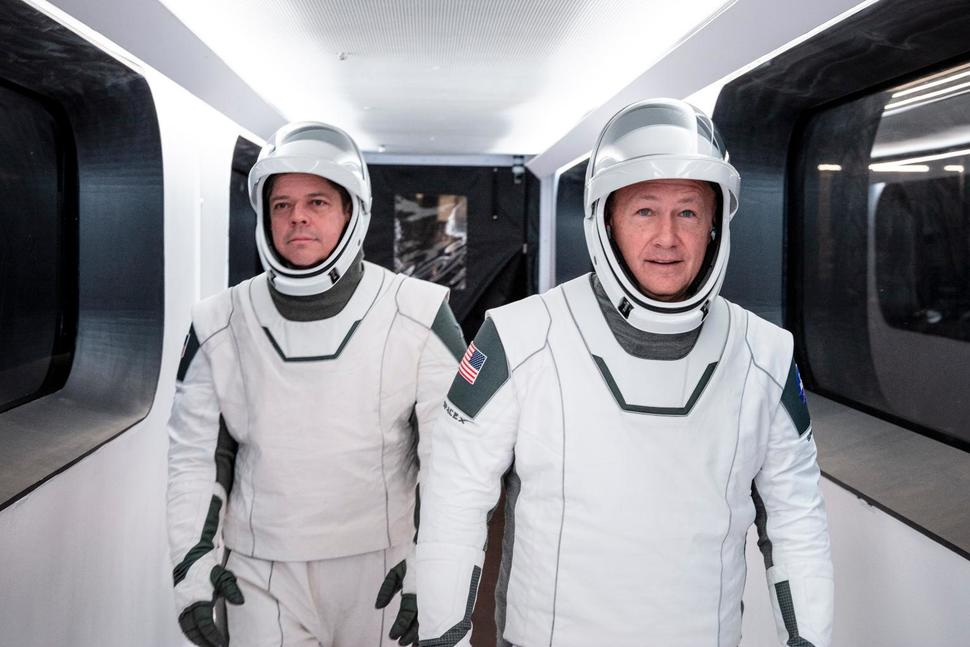
\includegraphics[max width=0.8\textwidth,max height=0.5\textheight]
    {{Images/spacex}.jpeg}
    \end{center}
}

\end{frame}
\endgroup{}

\begingroup{}
\begin{frame}[t]{Categories}
This week, you'll be answering questions in the following categories:
\begin{enumerate}
\item Aviation
\item Ireland
\item Colonial America
\item Famous Ships and Boats
\item Foreign Words and Phrases
\item Birds
\item Native Americans
\item The home of \ldots{}
\item Wonders of Engineering
\item Washington, D.C.
\end{enumerate}
\end{frame}
\endgroup{}

\begingroup{}
\begin{frame}
\vfill{}
\begin{beamercolorbox}[sep=8pt,center,shadow=true,rounded=true]{title}
\usebeamerfont{title}Good luck everyone! And have fun!
\end{beamercolorbox}
\vfill{}
\end{frame}
\endgroup{}
\def\thisSectionName{Aviation}
\section{Round 1}
\subsection*{Q1}
\begin{frame}[t]{Round 1 --- Aviation --- \mbox{Question 1}}
\vspace{-0.5em}
\begin{block}{Question}
In the U.\@S.\@, what is the minimum age at which you can be granted your private pilot's license for powered aircraft?
\end{block}
\end{frame}
\subsection*{Q2}
\begin{frame}[t]{Round 1 --- Aviation --- \mbox{Question 2}}
\vspace{-0.5em}
\begin{block}{Question}
Due to the shortage of aluminum during WWII, the Hughes Aircraft Company built an almost entirely wooden aircraft prototype, the H-4 Hercules. What nickname was it better known by?
\end{block}
\end{frame}
\subsection*{Q3}
\begin{frame}[t]{Round 1 --- Aviation --- \mbox{Question 3}}
\vspace{-0.5em}
\begin{block}{Question}
In the aviation world, what does ``FAA'' stand for?
\end{block}
\end{frame}
\subsection*{Q4}
\begin{frame}[t]{Round 1 --- Aviation --- \mbox{Question 4}}
\vspace{-0.5em}
\begin{columns}[T,totalwidth=\linewidth]
\begin{column}{0.32\linewidth}
\begin{block}{Question}
Give the aviation names of the three dimensions that an aircraft can rotate in, as pictured here. (You only need the names; you don't need to know which is which.)
\end{block}
\end{column}
\begin{column}{0.65\linewidth}
\begin{center}
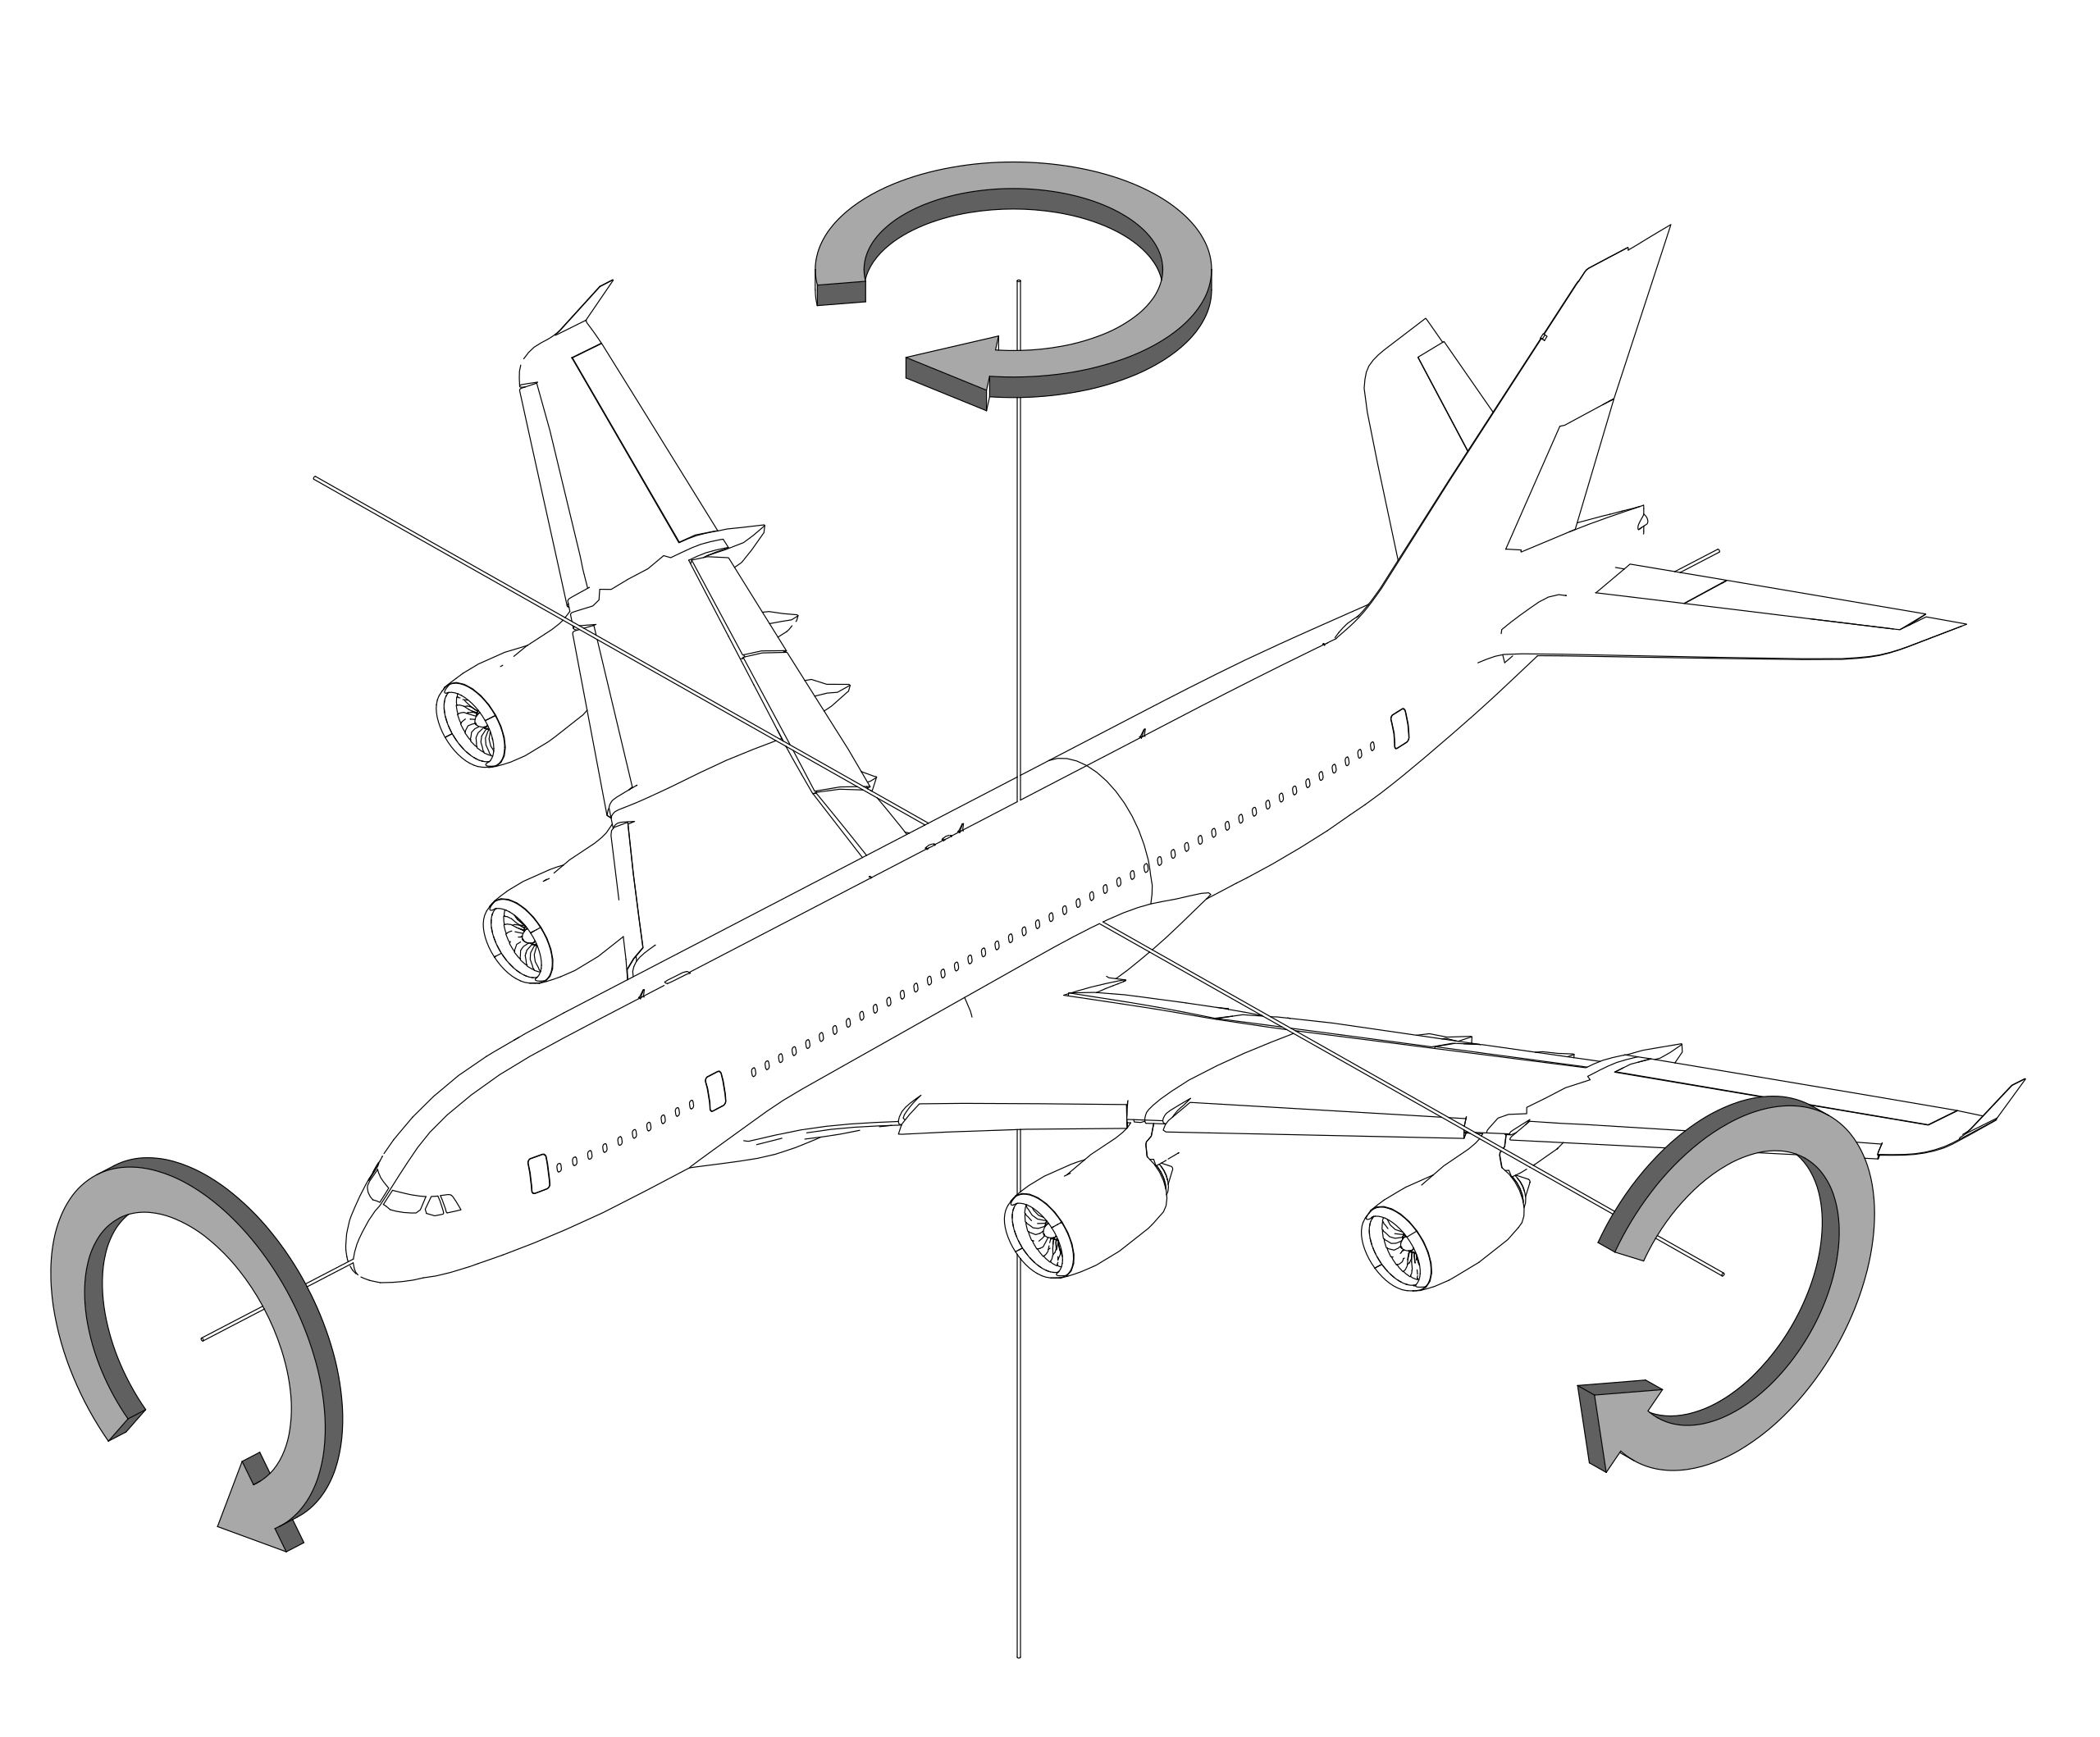
\includegraphics[max width=0.95\textwidth,max height=0.7\textheight]{{Images/rollpitchyaw}.png}
\end{center}
\end{column}
\end{columns}
\end{frame}
\subsection*{Q5}
\begin{frame}[t]{Round 1 --- Aviation --- \mbox{Question 5}}
\vspace{-0.5em}
\begin{block}{Question}
What was the name of the plane Charles Lindbergh flew on the first nonstop trans-Atlantic flight?
\end{block}
\end{frame}
\subsection*{Q6}
\begin{frame}[t]{Round 1 --- Aviation --- \mbox{Question 6}}
\vspace{-0.5em}
\begin{block}{Question}
In what year did the Wright Brothers complete their famous first flight of a heavier-than-air, powered aircraft?
\end{block}
\end{frame}
\subsection*{Q7}
\begin{frame}[t]{Round 1 --- Aviation --- \mbox{Question 7}}
\vspace{-0.5em}
\begin{columns}[T,totalwidth=\linewidth]
\begin{column}{0.32\linewidth}
\begin{block}{Question}
What is the name of the WWII-era fighter aircraft pictured here?
\end{block}
\end{column}
\begin{column}{0.65\linewidth}
\begin{center}
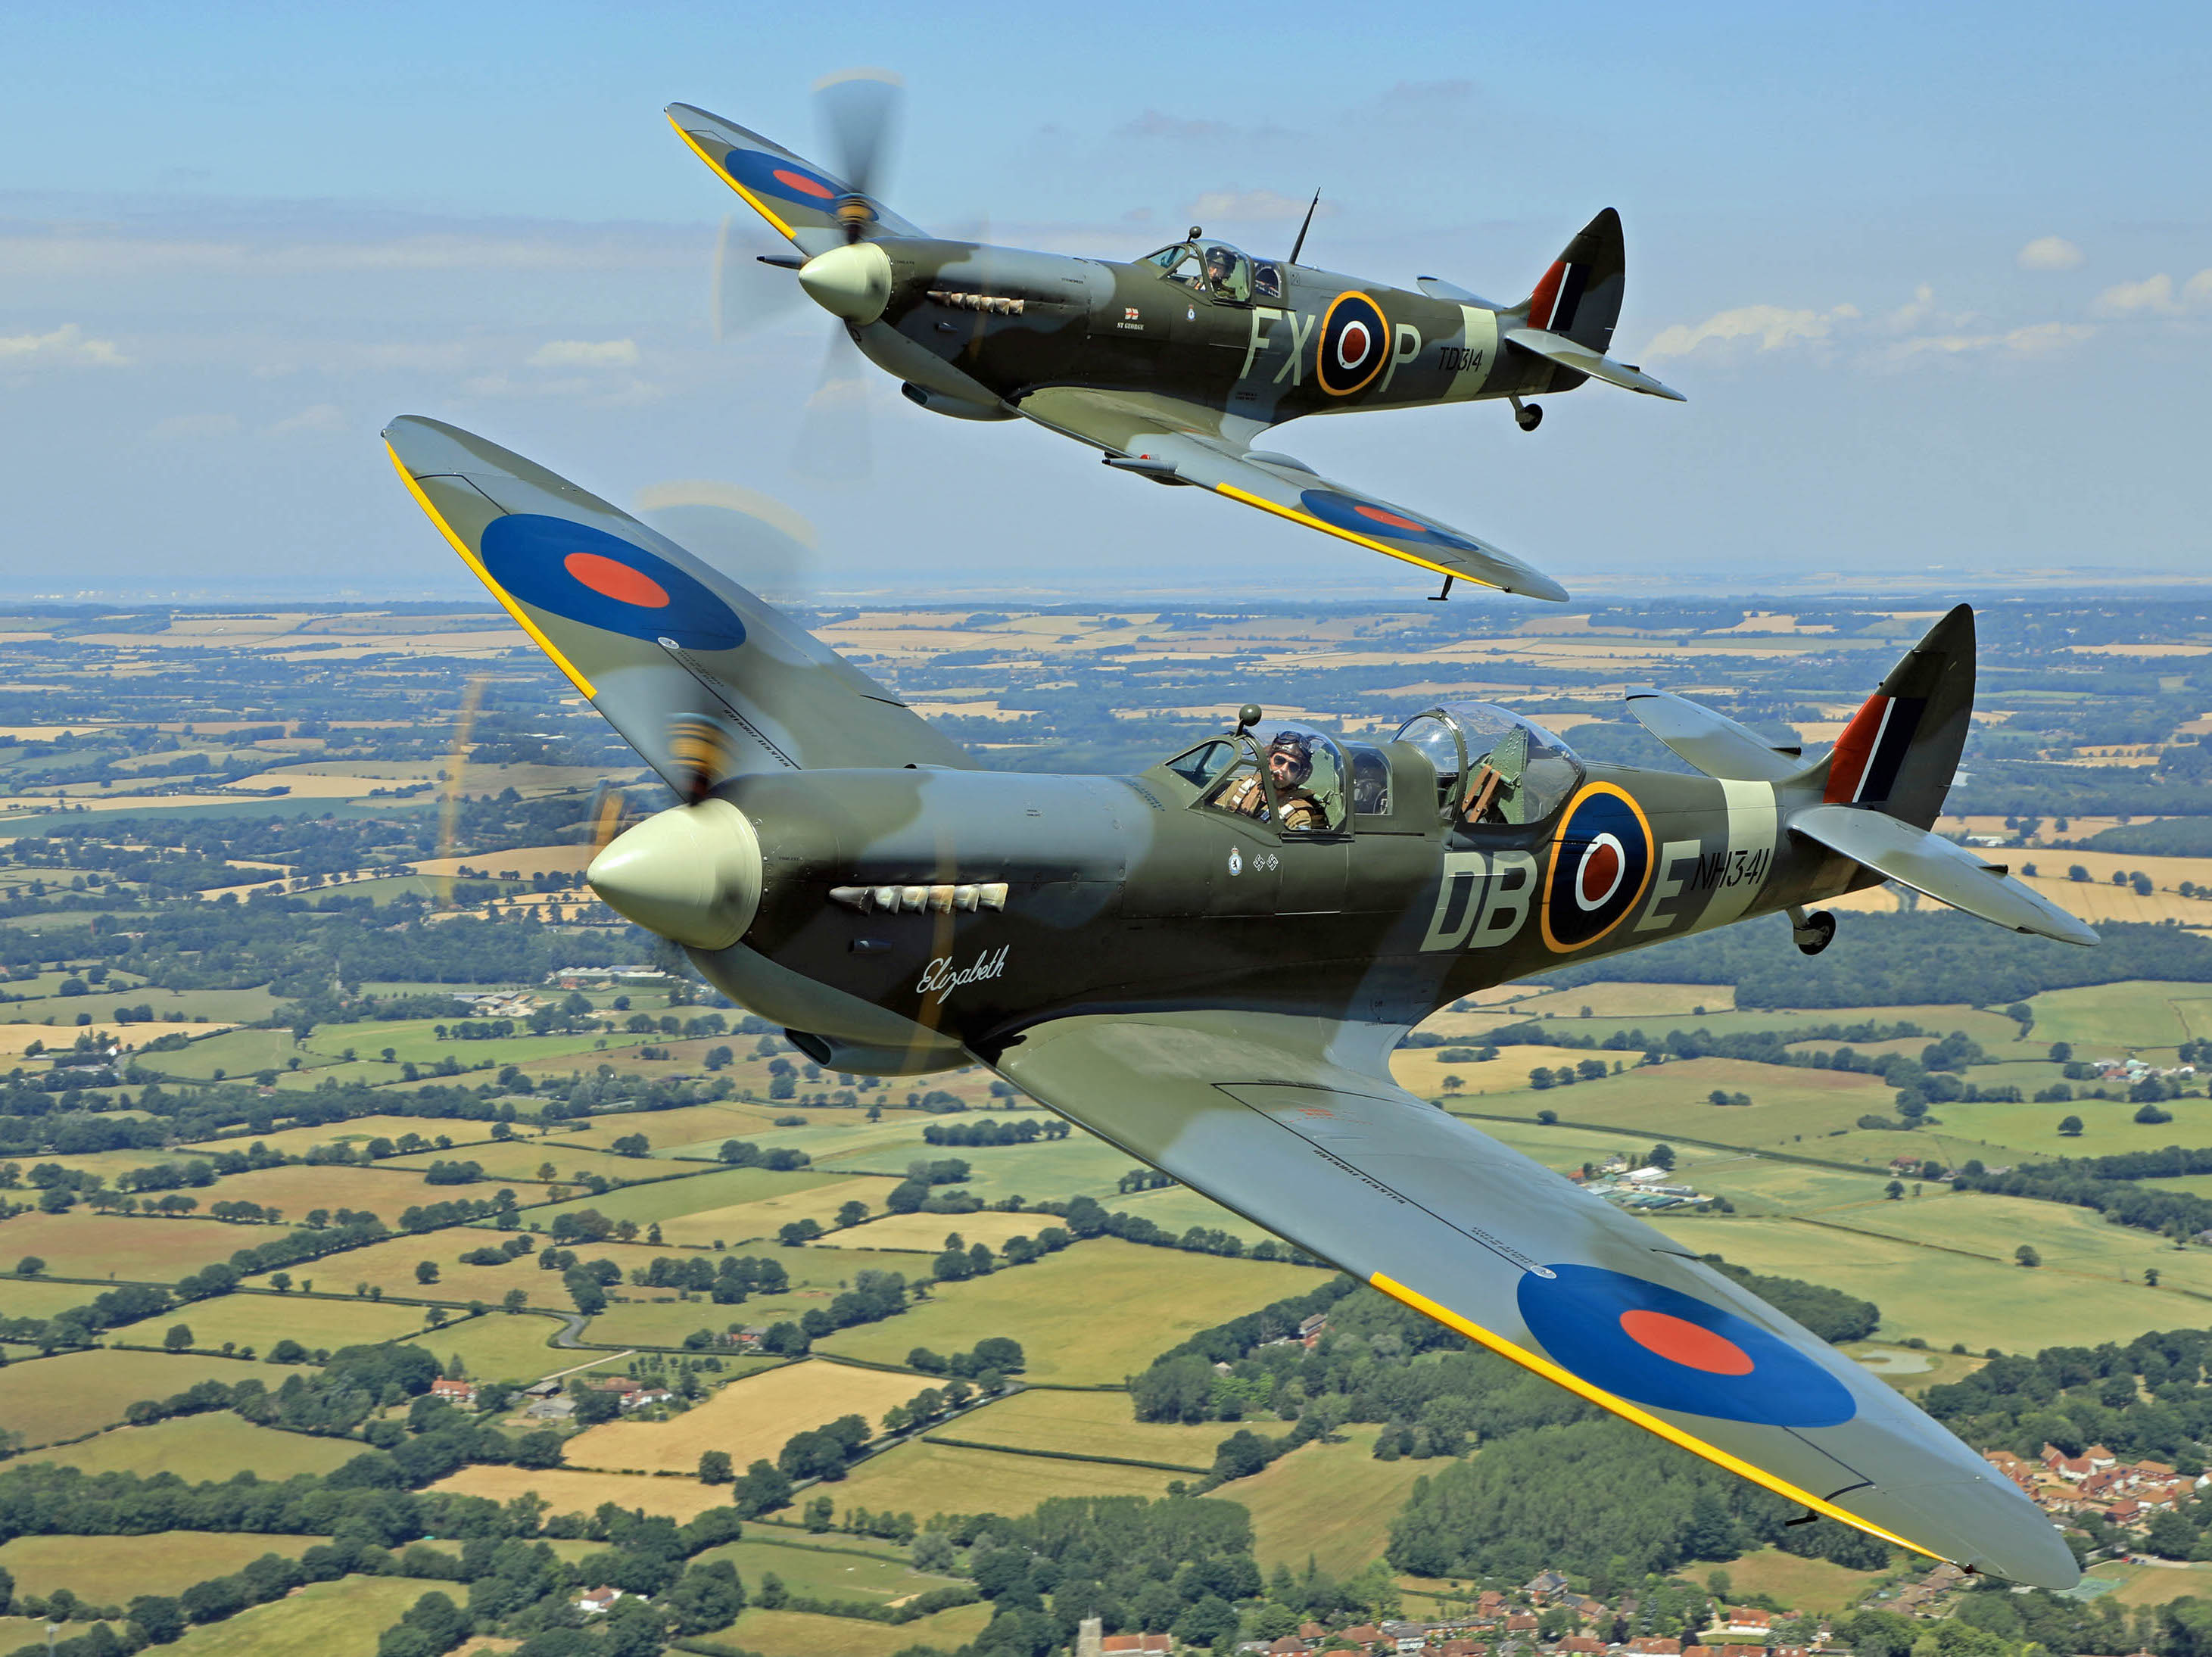
\includegraphics[max width=0.95\textwidth,max height=0.7\textheight]{{Images/spitfire}.jpg}
\end{center}
\end{column}
\end{columns}
\end{frame}
\subsection*{Q8}
\begin{frame}[t]{Round 1 --- Aviation --- \mbox{Question 8}}
\vspace{-0.5em}
\begin{block}{Question}
Whether measured by fleet size or number of passengers carried annually, which airline is the largest airline in the world?
\end{block}
\end{frame}
\subsection*{Q9}
\begin{frame}[t]{Round 1 --- Aviation --- \mbox{Question 9}}
\vspace{-0.5em}
\begin{block}{Question}
What was the name of the experimental airplane in which Chuck Yeager first broke the sound barrier?
\end{block}
\end{frame}
\subsection*{Q10}
\begin{frame}[t]{Round 1 --- Aviation --- \mbox{Question 10}}
\vspace{-0.5em}
\begin{columns}[T,totalwidth=\linewidth]
\begin{column}{0.32\linewidth}
\begin{block}{Question}
This isn't Boeing's logo; it's the logo of the company that merged with Boeing in 1997, whose logo Boeing modified slightly before adopting. Which (former) company's logo is it?
\end{block}
\end{column}
\begin{column}{0.65\linewidth}
\begin{center}

\includegraphics[max width=0.95\textwidth,max height=0.7\textheight]{{Images/mcdonnelldouglas}.png}
\end{center}
\end{column}
\end{columns}
\end{frame}
\subsection{Answers}
\begin{frame}[t]{Round 1 --- Aviation --- \mbox{Answer 1}}
\vspace{-0.5em}
\begin{block}{Question}
In the U.\@S.\@, what is the minimum age at which you can be granted your private pilot's license for powered aircraft?
\end{block}

\visible<2->{
    \begin{columns}[T,totalwidth=\linewidth]
    \begin{column}{0.32\linewidth}
    \begin{block}{Answer}
    17
    \end{block}
    \end{column}
    \begin{column}{0.65\linewidth}
    \begin{center}
    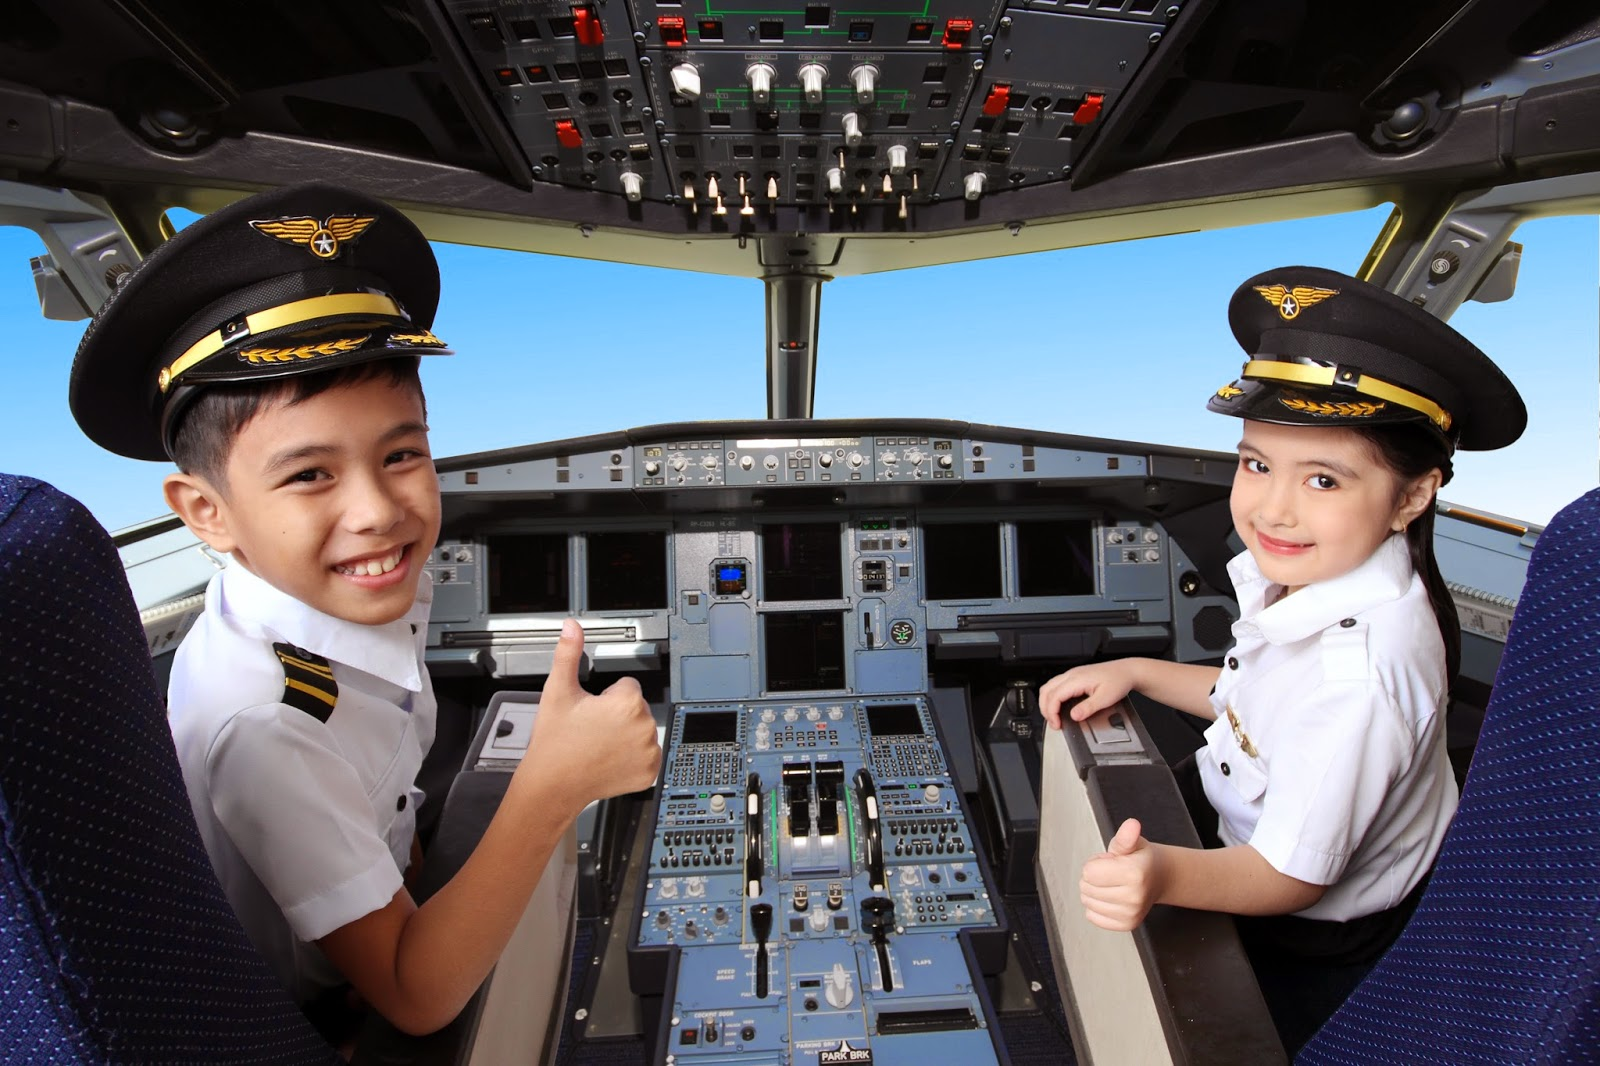
\includegraphics[max width=0.95\textwidth,
        max height=0.50000\textheight]{{Images/cockpit}.jpg}
    \end{center}
    \end{column}
    \end{columns}
}
\end{frame}
\begin{frame}[t]{Round 1 --- Aviation --- \mbox{Answer 2}}
\vspace{-0.5em}
\begin{block}{Question}
Due to the shortage of aluminum during WWII, the Hughes Aircraft Company built an almost entirely wooden aircraft prototype, the H-4 Hercules. What nickname was it better known by?
\end{block}

\visible<2->{
    \begin{columns}[T,totalwidth=\linewidth]
    \begin{column}{0.32\linewidth}
    \begin{block}{Answer}
    The \emph{Spruce Goose}
    \end{block}
    \end{column}
    \begin{column}{0.65\linewidth}
    \begin{center}
    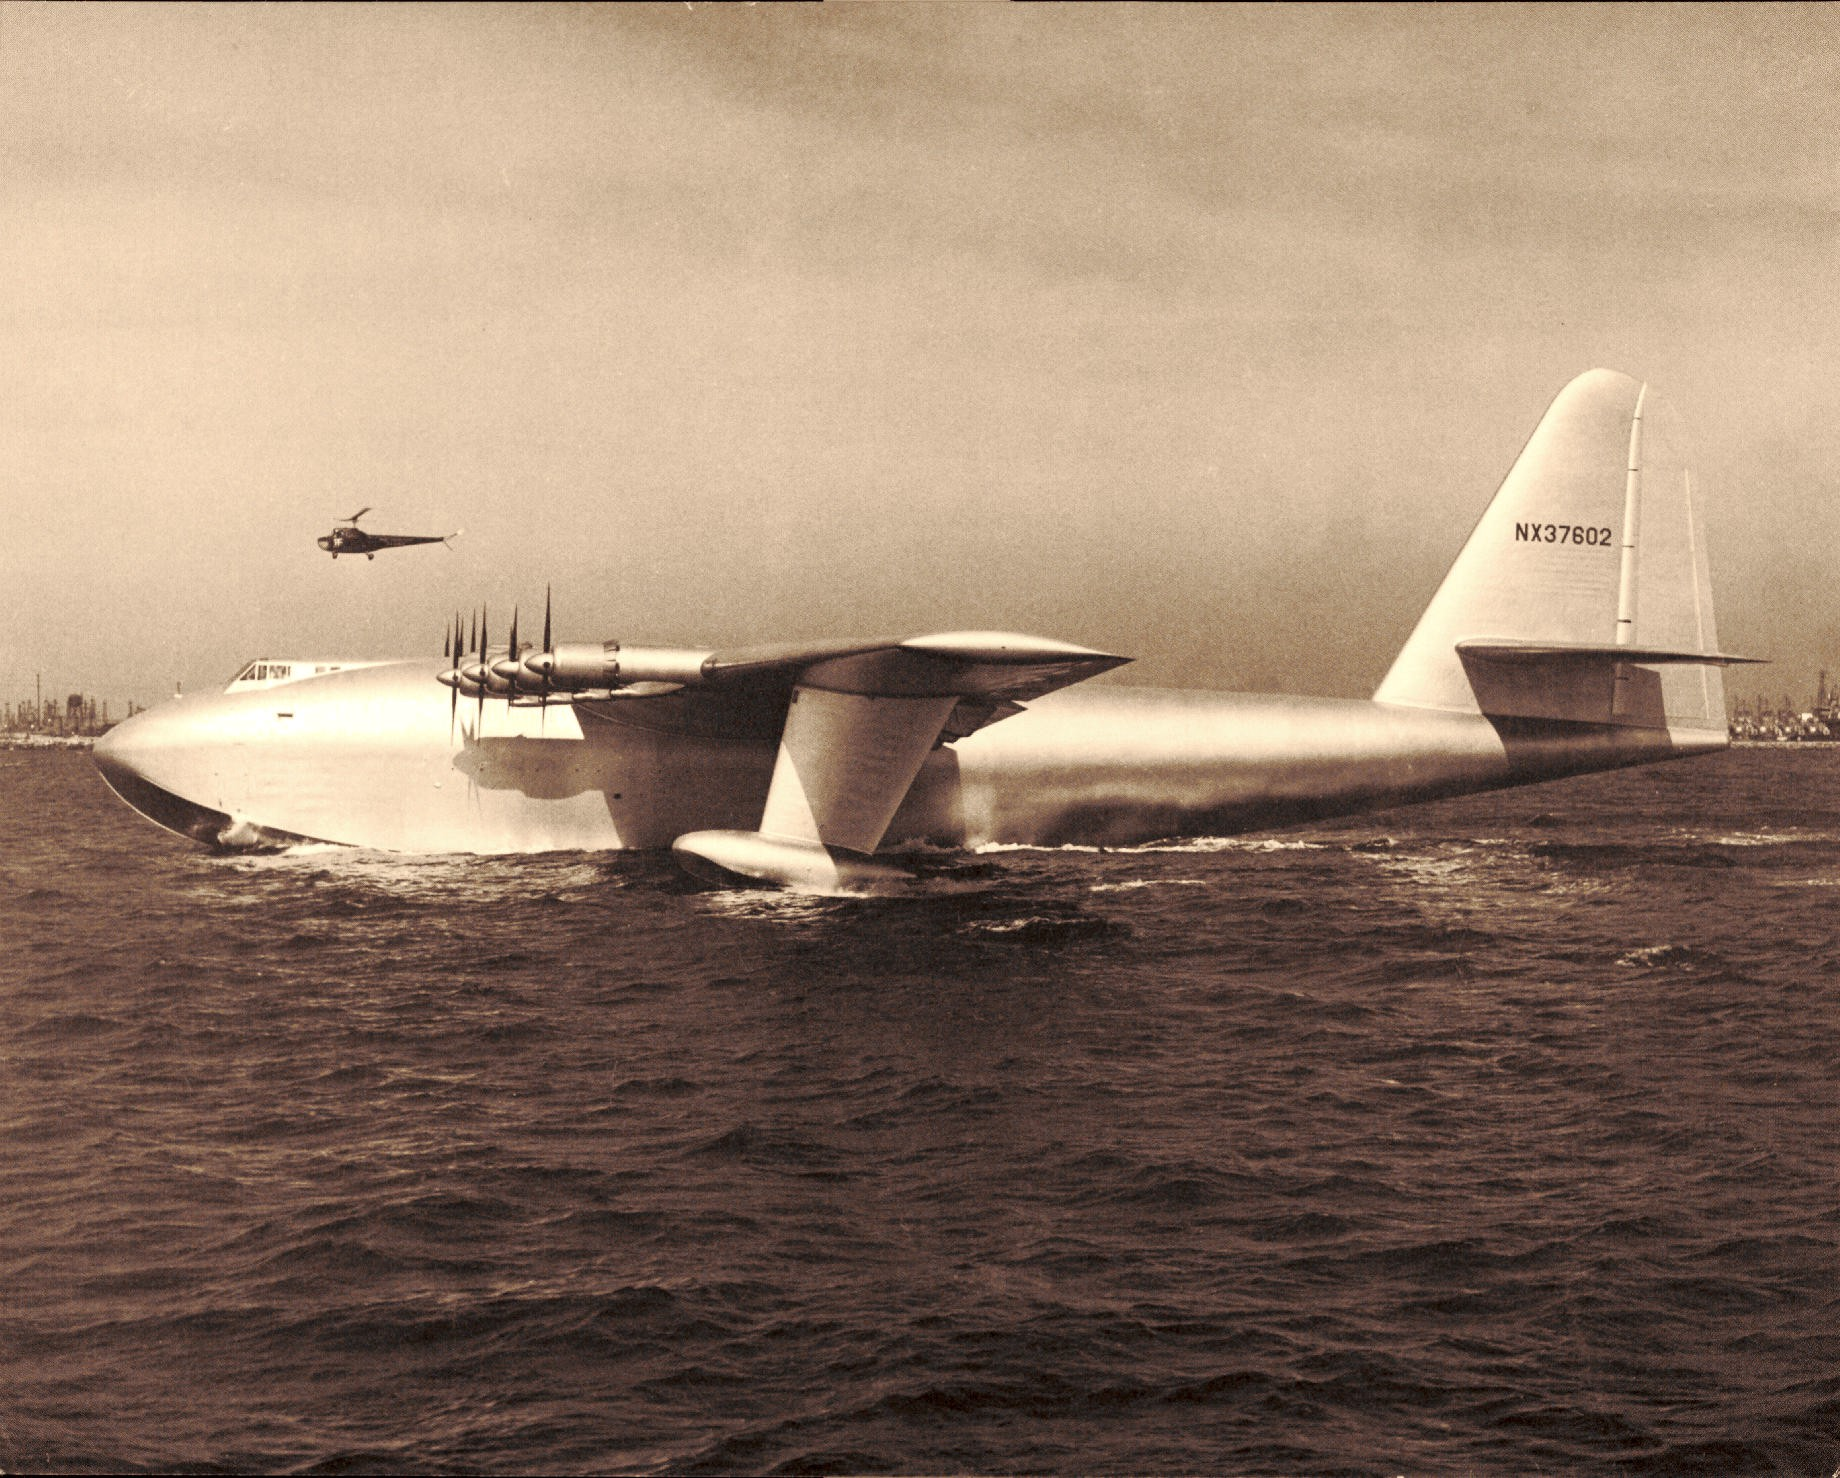
\includegraphics[max width=0.95\textwidth,
        max height=0.46000\textheight]{{Images/sprucegoose}.jpg}
    \end{center}
    \end{column}
    \end{columns}
}
\end{frame}
\begin{frame}[t]{Round 1 --- Aviation --- \mbox{Answer 3}}
\vspace{-0.5em}
\begin{block}{Question}
In the aviation world, what does ``FAA'' stand for?
\end{block}

\visible<2->{
    \begin{columns}[T,totalwidth=\linewidth]
    \begin{column}{0.32\linewidth}
    \begin{block}{Answer}
    Federal Aviation Administration
    \end{block}
    \end{column}
    \begin{column}{0.65\linewidth}
    \begin{center}
    
\includegraphics[max width=0.95\textwidth,
        max height=0.54000\textheight]{{Images/faa}.png}
    \end{center}
    \end{column}
    \end{columns}
}
\end{frame}
\begin{frame}[t]{Round 1 --- Aviation --- \mbox{Answer 4}}
\vspace{-0.5em}
\begin{columns}[T,totalwidth=\linewidth]
\begin{column}{0.32\linewidth}
\begin{block}{Question}
Give the aviation names of the three dimensions that an aircraft can rotate in, as pictured here. (You only need the names; you don't need to know which is which.)
\end{block}
\visible<2->{
    \begin{block}{Answer}
    Roll, pitch, and yaw
    \end{block}
}
\end{column}
\begin{column}{0.65\linewidth}
\begin{center}
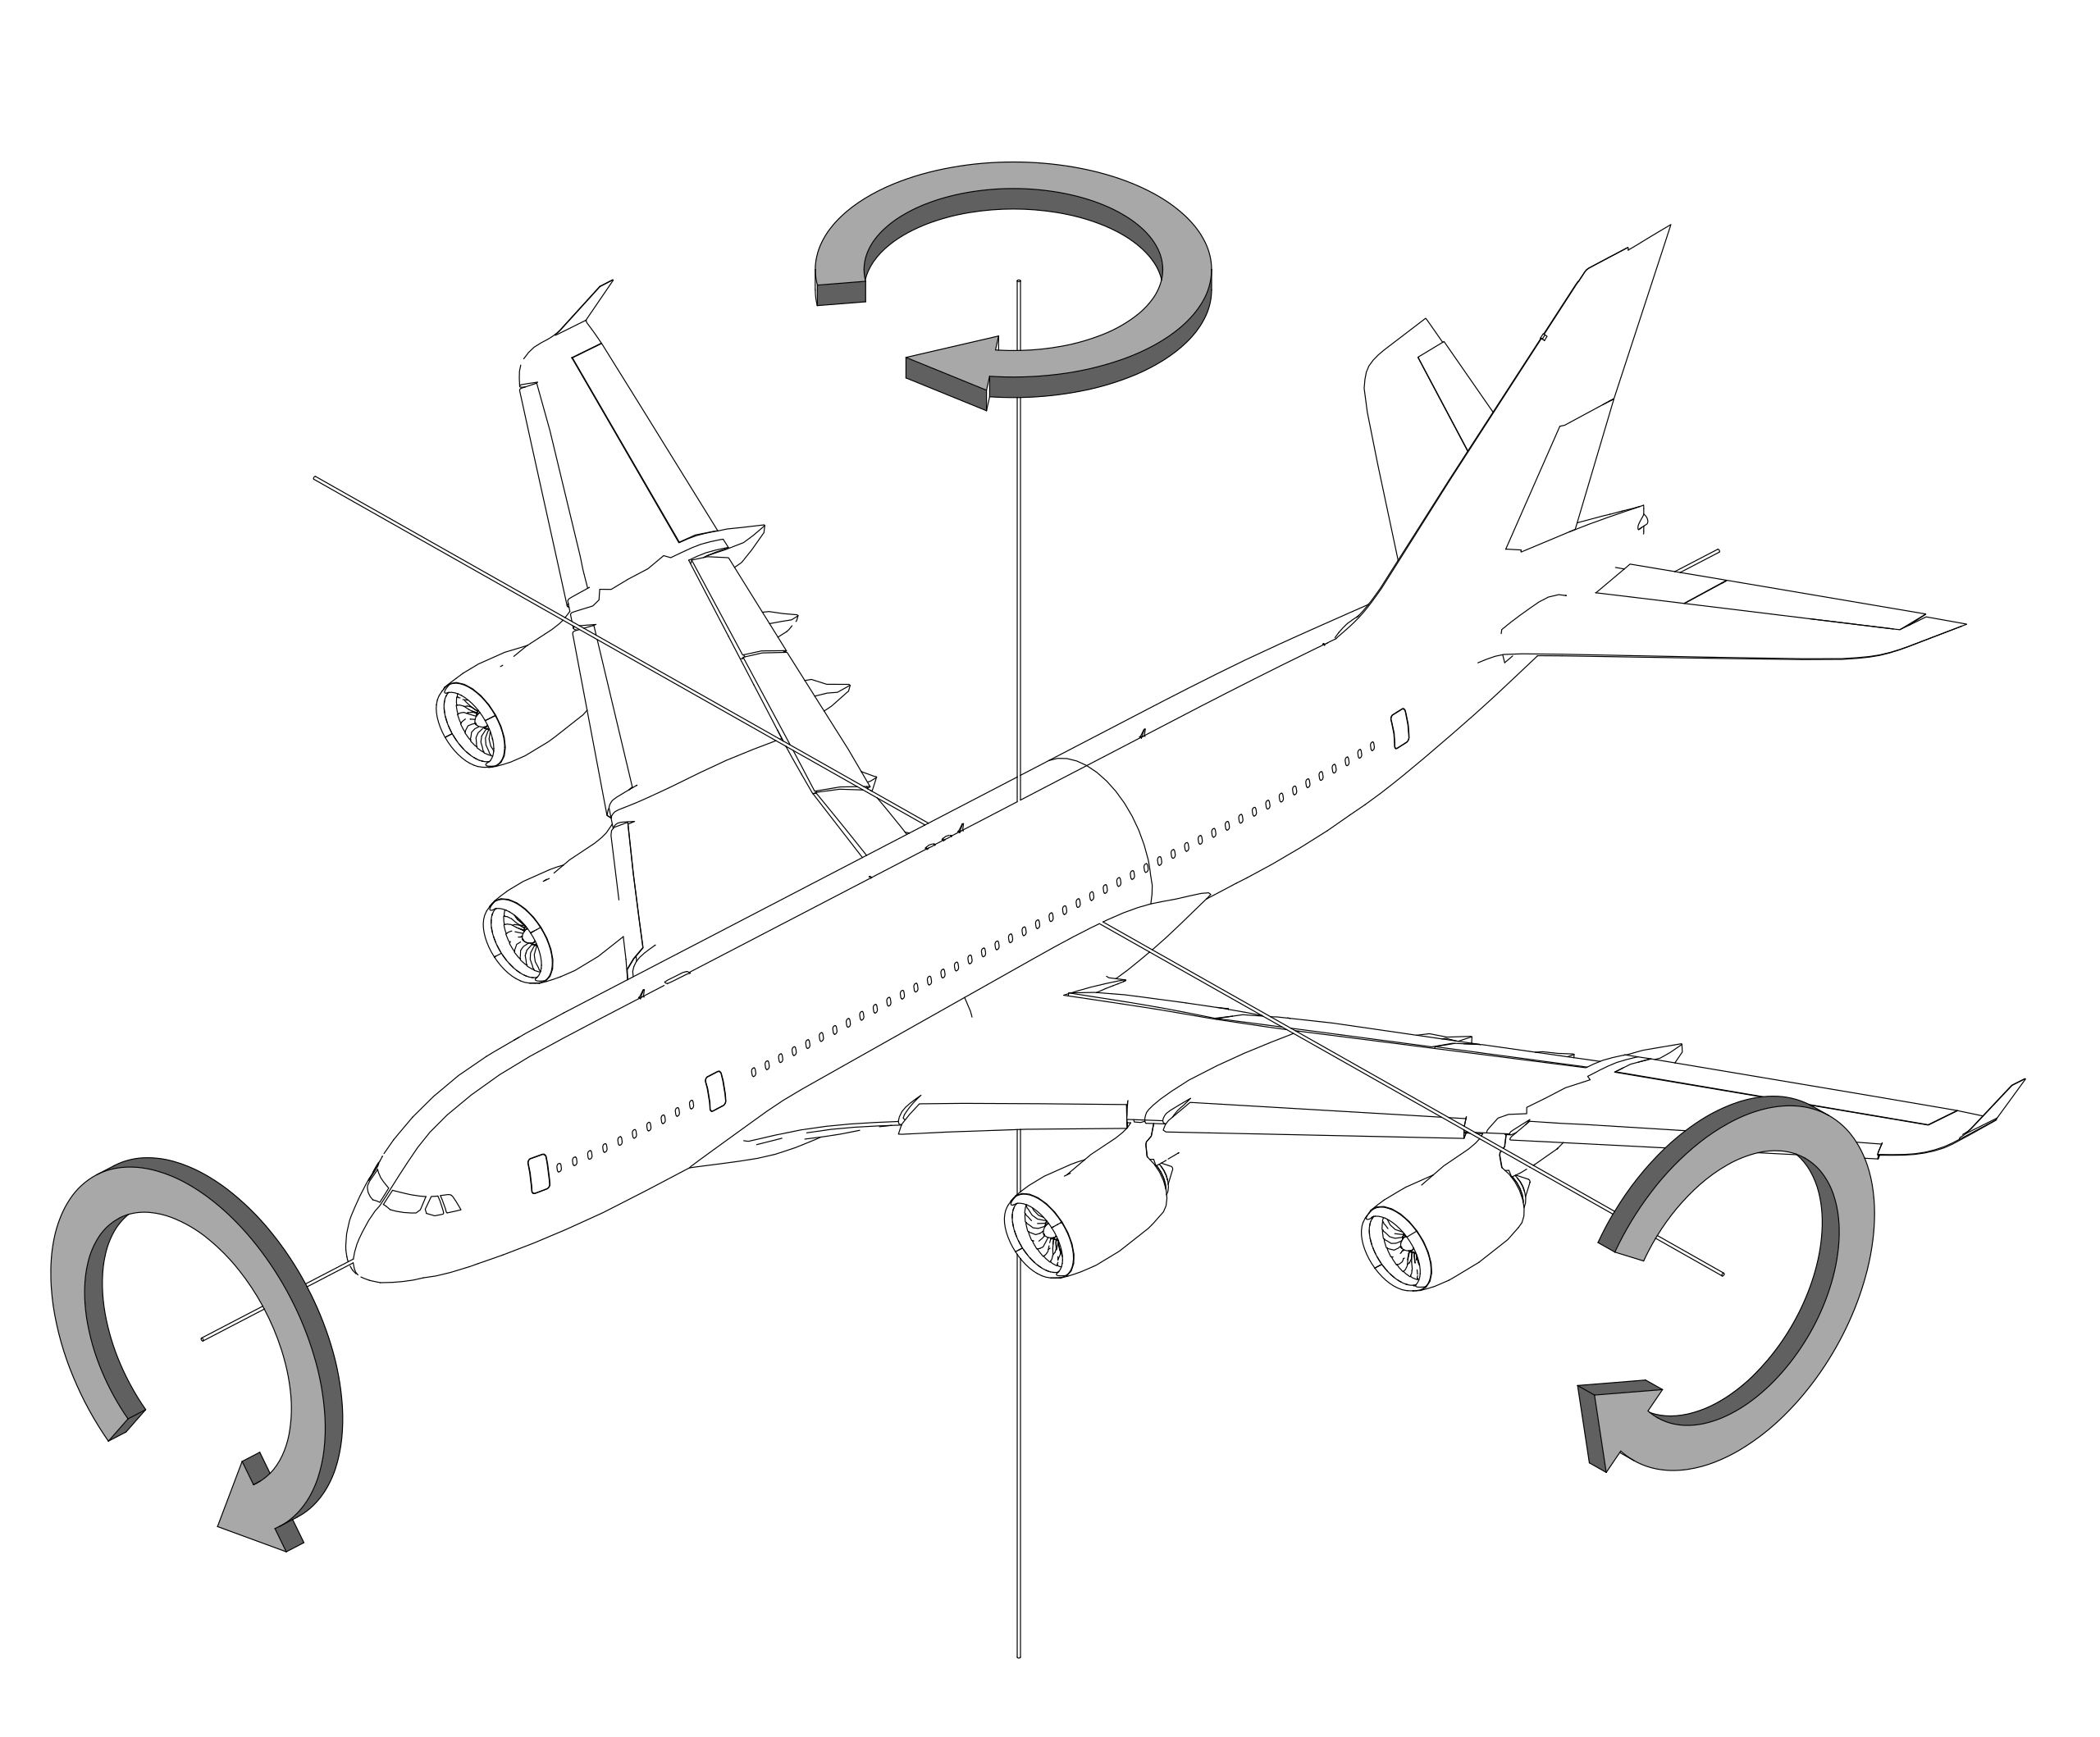
\includegraphics[max width=0.95\textwidth,max height=0.7\textheight]{{Images/rollpitchyaw}.png}
\end{center}
\end{column}
\end{columns}
\end{frame}
\begin{frame}[t]{Round 1 --- Aviation --- \mbox{Answer 5}}
\vspace{-0.5em}
\begin{block}{Question}
What was the name of the plane Charles Lindbergh flew on the first nonstop trans-Atlantic flight?
\end{block}

\visible<2->{
    \begin{columns}[T,totalwidth=\linewidth]
    \begin{column}{0.32\linewidth}
    \begin{block}{Answer}
    The \emph{Spirit of St.\ Louis}
    \end{block}
    \end{column}
    \begin{column}{0.65\linewidth}
    \begin{center}
    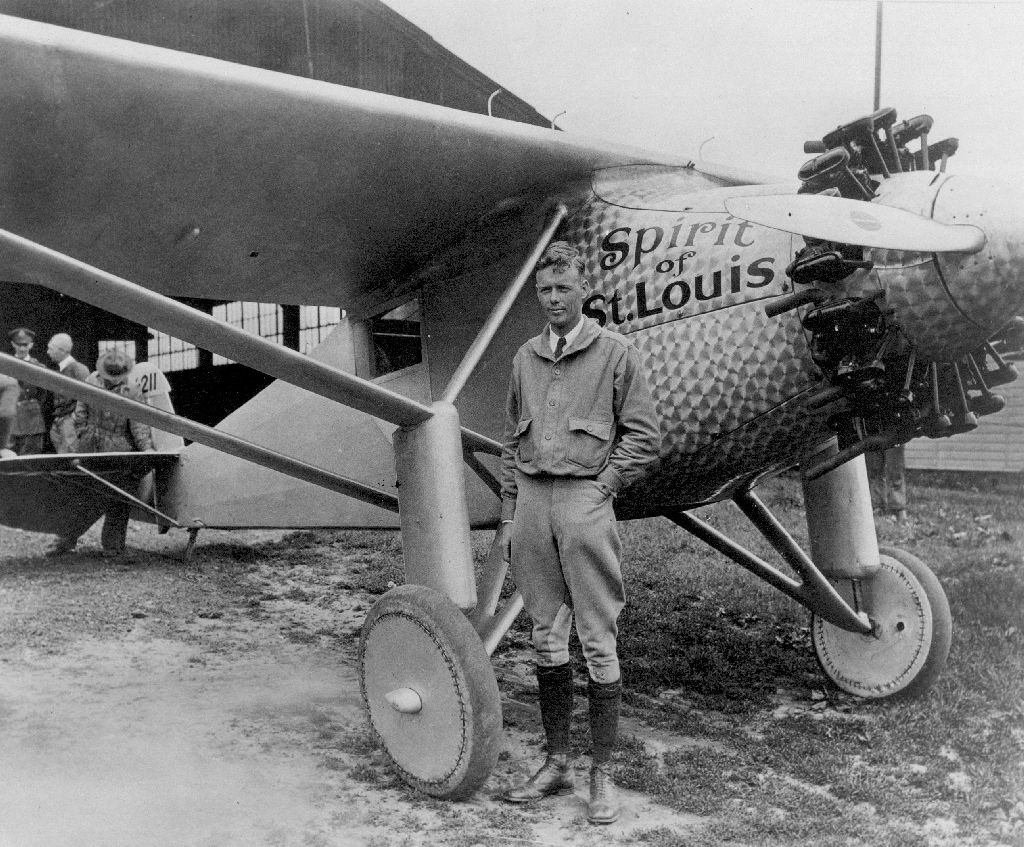
\includegraphics[max width=0.95\textwidth,
        max height=0.54000\textheight]{{Images/lindbergh}.jpg}
    \end{center}
    \end{column}
    \end{columns}
}
\end{frame}
\begin{frame}[t]{Round 1 --- Aviation --- \mbox{Answer 6}}
\vspace{-0.5em}
\begin{block}{Question}
In what year did the Wright Brothers complete their famous first flight of a heavier-than-air, powered aircraft?
\end{block}

\visible<2->{
    \begin{columns}[T,totalwidth=\linewidth]
    \begin{column}{0.32\linewidth}
    \begin{block}{Answer}
    1903
    \end{block}
    \end{column}
    \begin{column}{0.65\linewidth}
    \begin{center}
    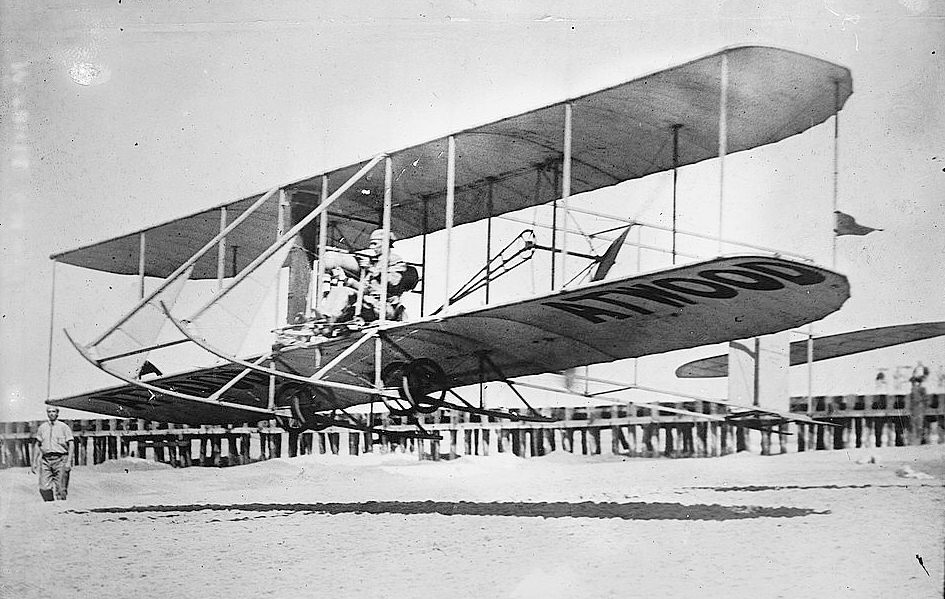
\includegraphics[max width=0.95\textwidth,
        max height=0.50000\textheight]{{Images/biplane}.jpg}
    \end{center}
    \end{column}
    \end{columns}
}
\end{frame}
\begin{frame}[t]{Round 1 --- Aviation --- \mbox{Answer 7}}
\vspace{-0.5em}
\begin{columns}[T,totalwidth=\linewidth]
\begin{column}{0.32\linewidth}
\begin{block}{Question}
What is the name of the WWII-era fighter aircraft pictured here?
\end{block}
\visible<2->{
    \begin{block}{Answer}
    Spitfire / Submarine Spitfire
    \end{block}
}
\end{column}
\begin{column}{0.65\linewidth}
\begin{center}
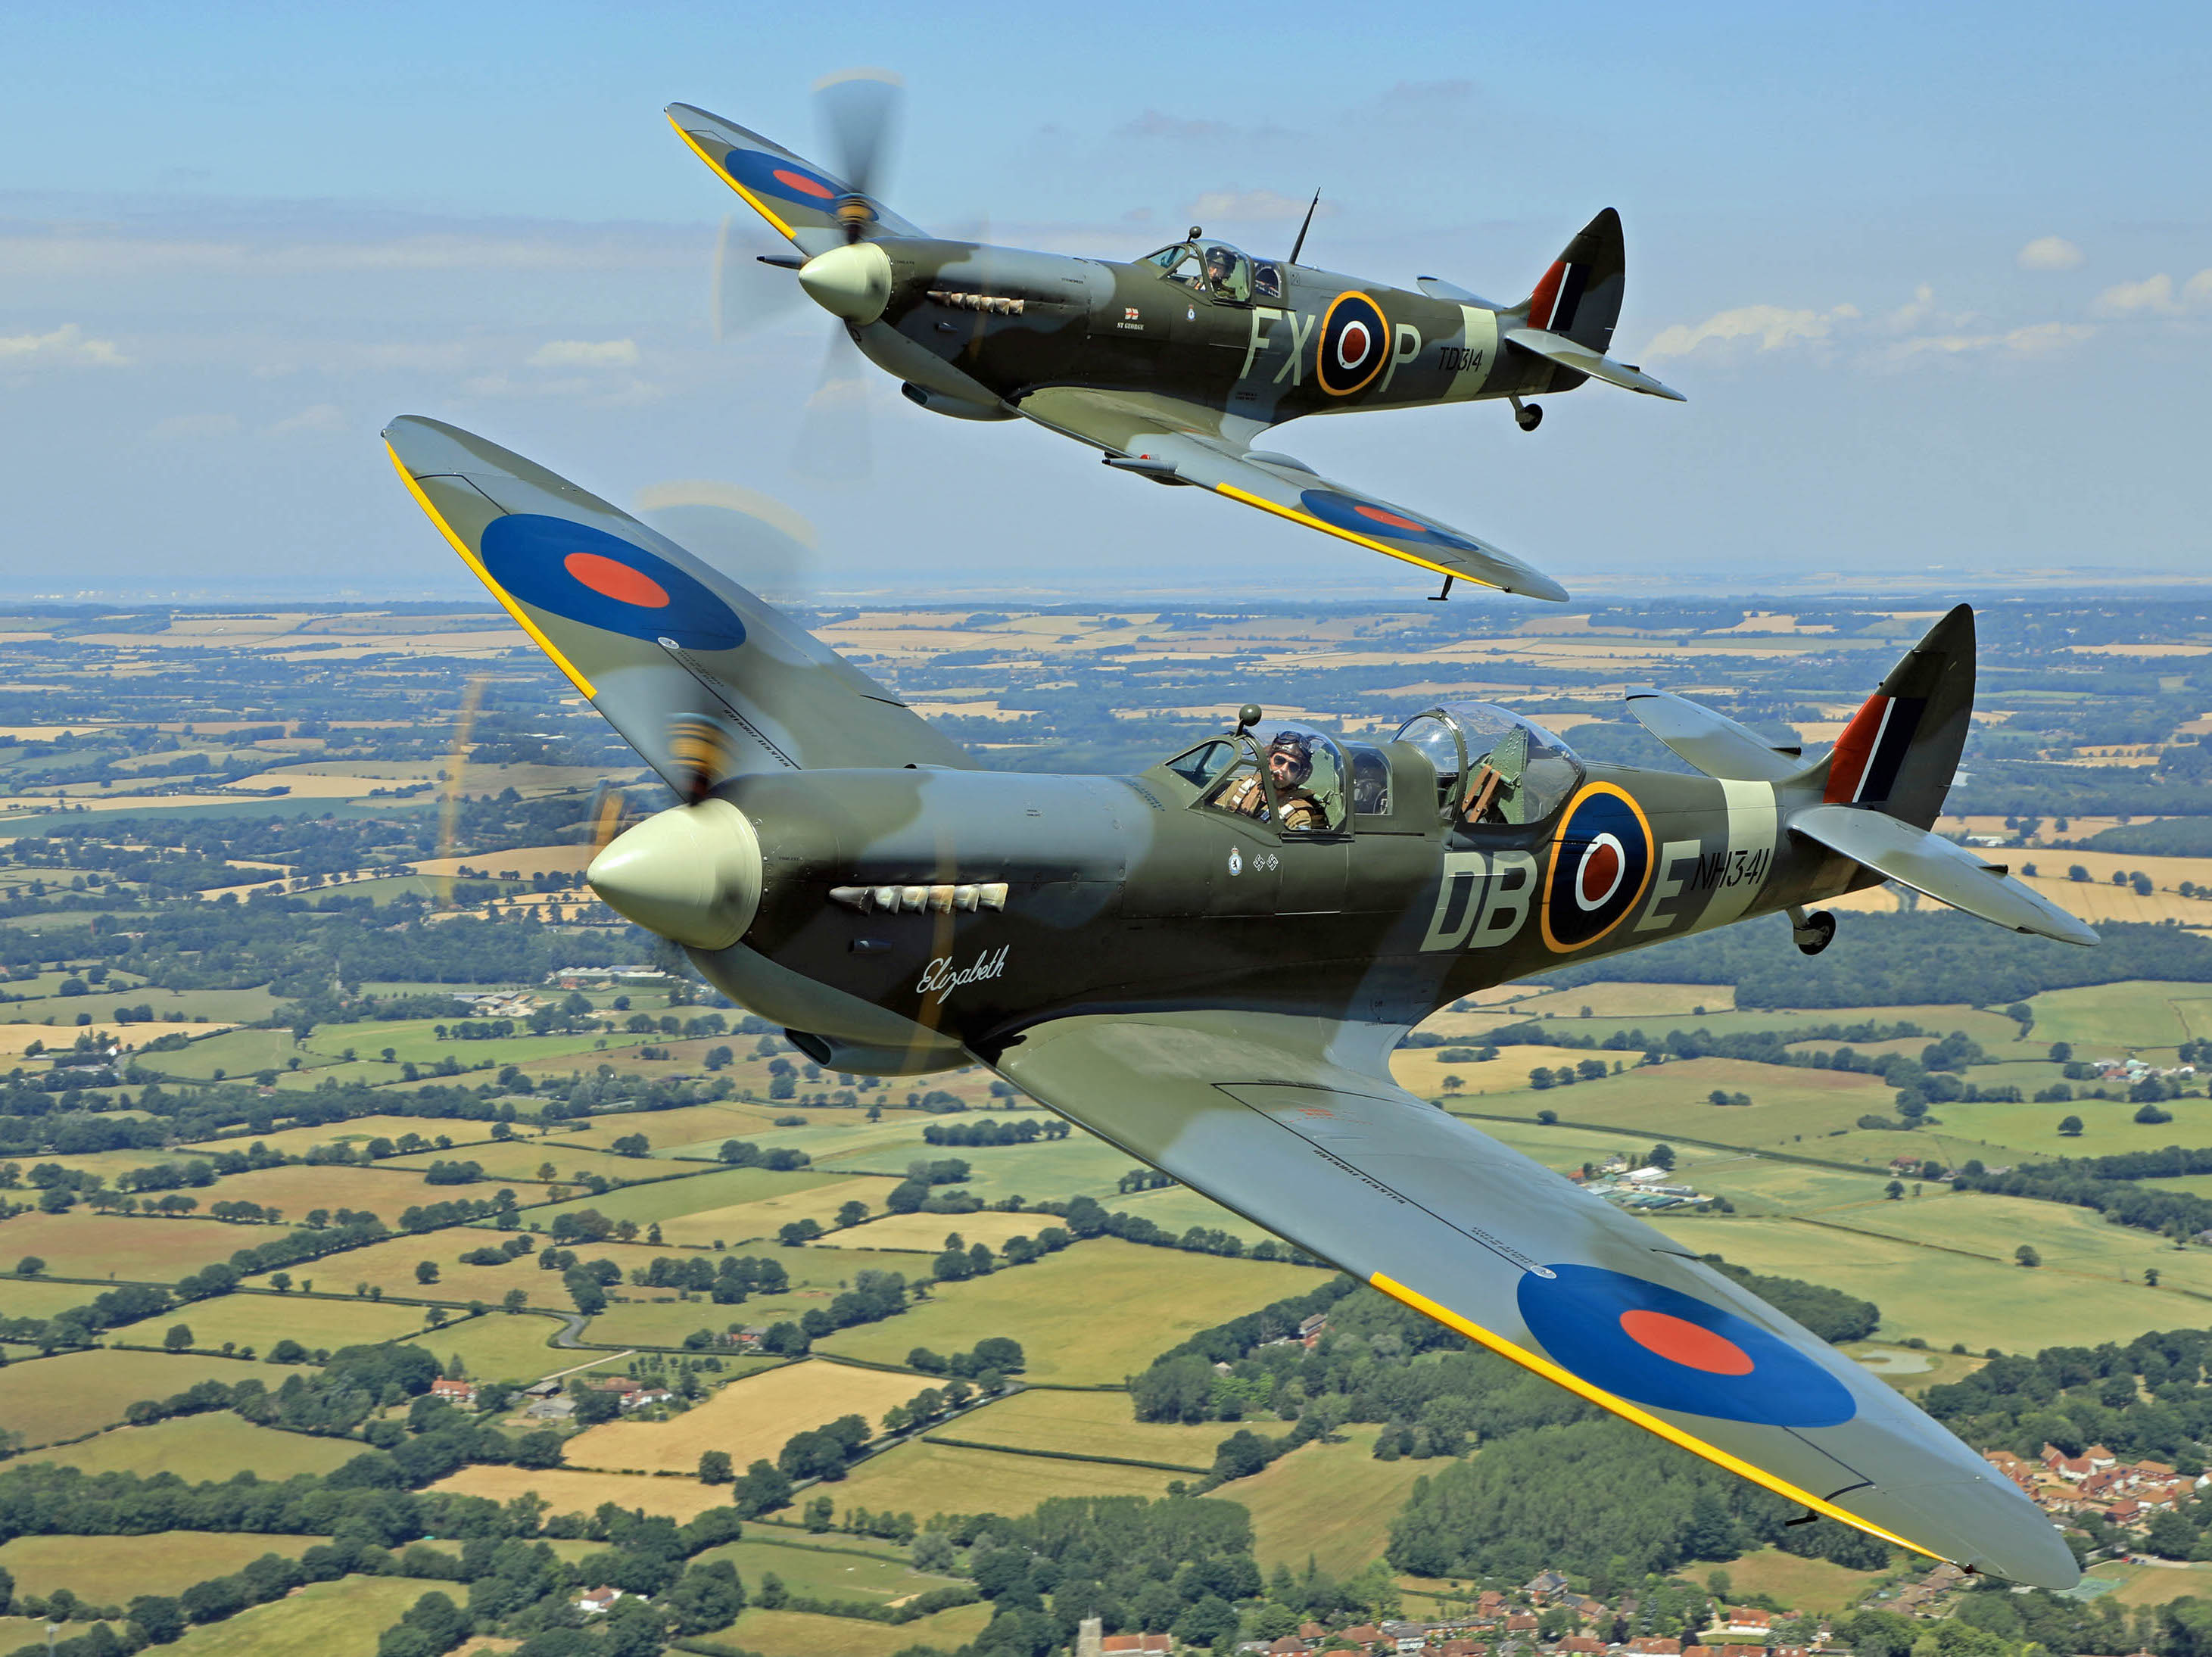
\includegraphics[max width=0.95\textwidth,max height=0.7\textheight]{{Images/spitfire}.jpg}
\end{center}
\end{column}
\end{columns}
\end{frame}
\begin{frame}[t]{Round 1 --- Aviation --- \mbox{Answer 8}}
\vspace{-0.5em}
\begin{block}{Question}
Whether measured by fleet size or number of passengers carried annually, which airline is the largest airline in the world?
\end{block}

\visible<2->{
    \begin{columns}[T,totalwidth=\linewidth]
    \begin{column}{0.32\linewidth}
    \begin{block}{Answer}
    American Airlines
    \end{block}
    \end{column}
    \begin{column}{0.65\linewidth}
    \begin{center}
    
\includegraphics[max width=0.95\textwidth,
        max height=0.50000\textheight]{{Images/aa}.png}
    \end{center}
    \end{column}
    \end{columns}
}
\end{frame}
\begin{frame}[t]{Round 1 --- Aviation --- \mbox{Answer 9}}
\vspace{-0.5em}
\begin{block}{Question}
What was the name of the experimental airplane in which Chuck Yeager first broke the sound barrier?
\end{block}

\visible<2->{
    \begin{columns}[T,totalwidth=\linewidth]
    \begin{column}{0.32\linewidth}
    \begin{block}{Answer}
    Bell X-1
    \end{block}
    \end{column}
    \begin{column}{0.65\linewidth}
    \begin{center}
    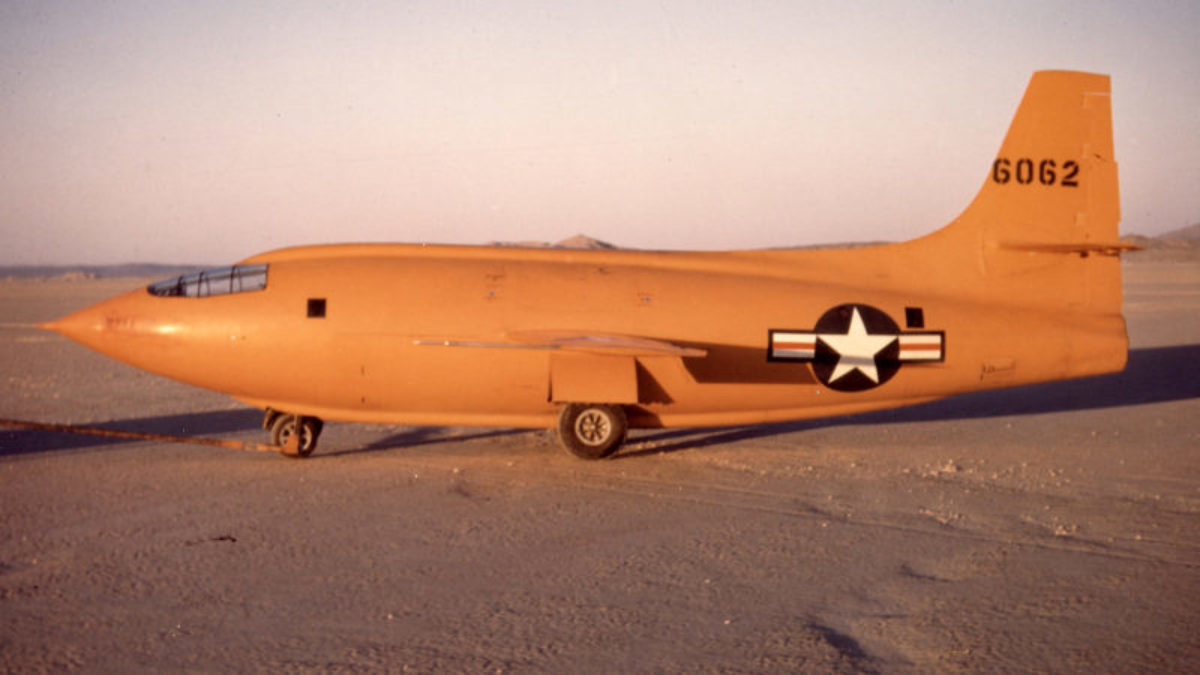
\includegraphics[max width=0.95\textwidth,
        max height=0.54000\textheight]{{Images/bellx1}.jpg}
    \end{center}
    \end{column}
    \end{columns}
}
\end{frame}
\begin{frame}[t]{Round 1 --- Aviation --- \mbox{Answer 10}}
\vspace{-0.5em}
\begin{columns}[T,totalwidth=\linewidth]
\begin{column}{0.32\linewidth}
\begin{block}{Question}
This isn't Boeing's logo; it's the logo of the company that merged with Boeing in 1997, whose logo Boeing modified slightly before adopting. Which (former) company's logo is it?
\end{block}
\visible<2->{
    \begin{block}{Answer}
    McDonnell Douglas
    \end{block}
}
\end{column}
\begin{column}{0.65\linewidth}
\begin{center}

\includegraphics[max width=0.95\textwidth,max height=0.7\textheight]{{Images/mcdonnelldouglas}.png}
\end{center}
\end{column}
\end{columns}
\end{frame}
\def\thisSectionName{Ireland}
\section{Round 2}
\subsection*{Q1}
\begin{frame}[t]{Round 2 --- Ireland --- \mbox{Question 1}}
\vspace{-0.5em}
\begin{block}{Question}
People bend over backwards to visit this tourist attraction in Ireland and then they presumably gab about their visit. What is the tourist attraction?
\end{block}
\end{frame}
\subsection*{Q2}
\begin{frame}[t]{Round 2 --- Ireland --- \mbox{Question 2}}
\vspace{-0.5em}
\begin{block}{Question}
How many counties are there in the Republic of Ireland?
\end{block}
\end{frame}
\subsection*{Q3}
\begin{frame}[t]{Round 2 --- Ireland --- \mbox{Question 3}}
\vspace{-0.5em}
\begin{block}{Question}
What is the name of the famous Irish crystal that takes its name from the city in which it is produced?
\end{block}
\end{frame}
\subsection*{Q4}
\begin{frame}[t]{Round 2 --- Ireland --- \mbox{Question 4}}
\vspace{-0.5em}
\begin{block}{Question}
What is the name of the northernmost peninsula in County Kerry, known for its stunningly beautiful scenery?
\end{block}
\end{frame}
\subsection*{Q5}
\begin{frame}[t]{Round 2 --- Ireland --- \mbox{Question 5}}
\vspace{-0.5em}
\begin{block}{Question}
By population, what is the second largest city in Ireland?
\end{block}
\end{frame}
\subsection*{Q6}
\begin{frame}[t]{Round 2 --- Ireland --- \mbox{Question 6}}
\vspace{-0.5em}
\begin{block}{Question}
In what year did the Irish win their independence from Great Britain?
\end{block}
\end{frame}
\subsection*{Q7}
\begin{frame}[t]{Round 2 --- Ireland --- \mbox{Question 7}}
\vspace{-0.5em}
\begin{block}{Question}
What  is the name of the Yeats poem that includes the repeated line, ``A terrible beauty is born''?
\end{block}
\end{frame}
\subsection*{Q8}
\begin{frame}[t]{Round 2 --- Ireland --- \mbox{Question 8}}
\vspace{-0.5em}
\begin{block}{Question}
What famous oratorio, performed annually around the world to this day, had its debut at The Great Music Hall in Dublin during lent in 1742? 
\end{block}
\end{frame}
\subsection*{Q9}
\begin{frame}[t]{Round 2 --- Ireland --- \mbox{Question 9}}
\vspace{-0.5em}
\begin{block}{Question}
What was Yogi Berra's reported response to being told that Robert Briscoe, the Lord Mayor of Dublin, was Jewish?
\end{block}
\end{frame}
\subsection*{Q10}
\begin{frame}[t]{Round 2 --- Ireland --- \mbox{Question 10}}
\vspace{-0.5em}
\begin{block}{Question}
According to legend, what animal did St.\ Patrick drive out of Ireland?
\end{block}
\end{frame}
\subsection{Answers}
\begin{frame}[t]{Round 2 --- Ireland --- \mbox{Answer 1}}
\vspace{-0.5em}
\begin{block}{Question}
People bend over backwards to visit this tourist attraction in Ireland and then they presumably gab about their visit. What is the tourist attraction?
\end{block}

\visible<2->{
    \begin{columns}[T,totalwidth=\linewidth]
    \begin{column}{0.32\linewidth}
    \begin{block}{Answer}
    The Blarney Stone
    \end{block}
    \end{column}
    \begin{column}{0.65\linewidth}
    \begin{center}
    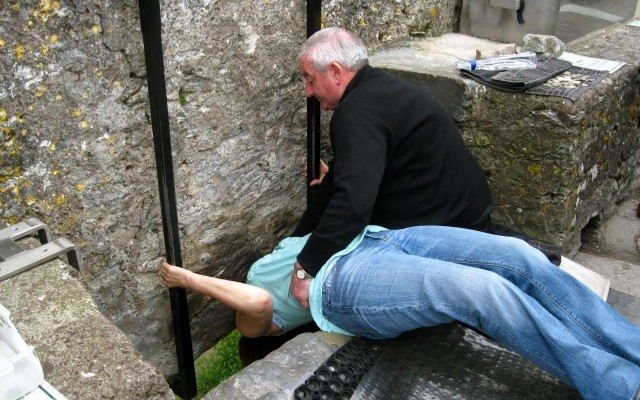
\includegraphics[max width=0.95\textwidth,
        max height=0.50000\textheight]{{Images/blarney}.jpg}
    \end{center}
    \end{column}
    \end{columns}
}
\end{frame}
\begin{frame}[t]{Round 2 --- Ireland --- \mbox{Answer 2}}
\vspace{-0.5em}
\begin{block}{Question}
How many counties are there in the Republic of Ireland?
\end{block}

\visible<2->{
    \begin{columns}[T,totalwidth=\linewidth]
    \begin{column}{0.32\linewidth}
    \begin{block}{Answer}
    26
    \end{block}
    \end{column}
    \begin{column}{0.65\linewidth}
    \begin{center}
    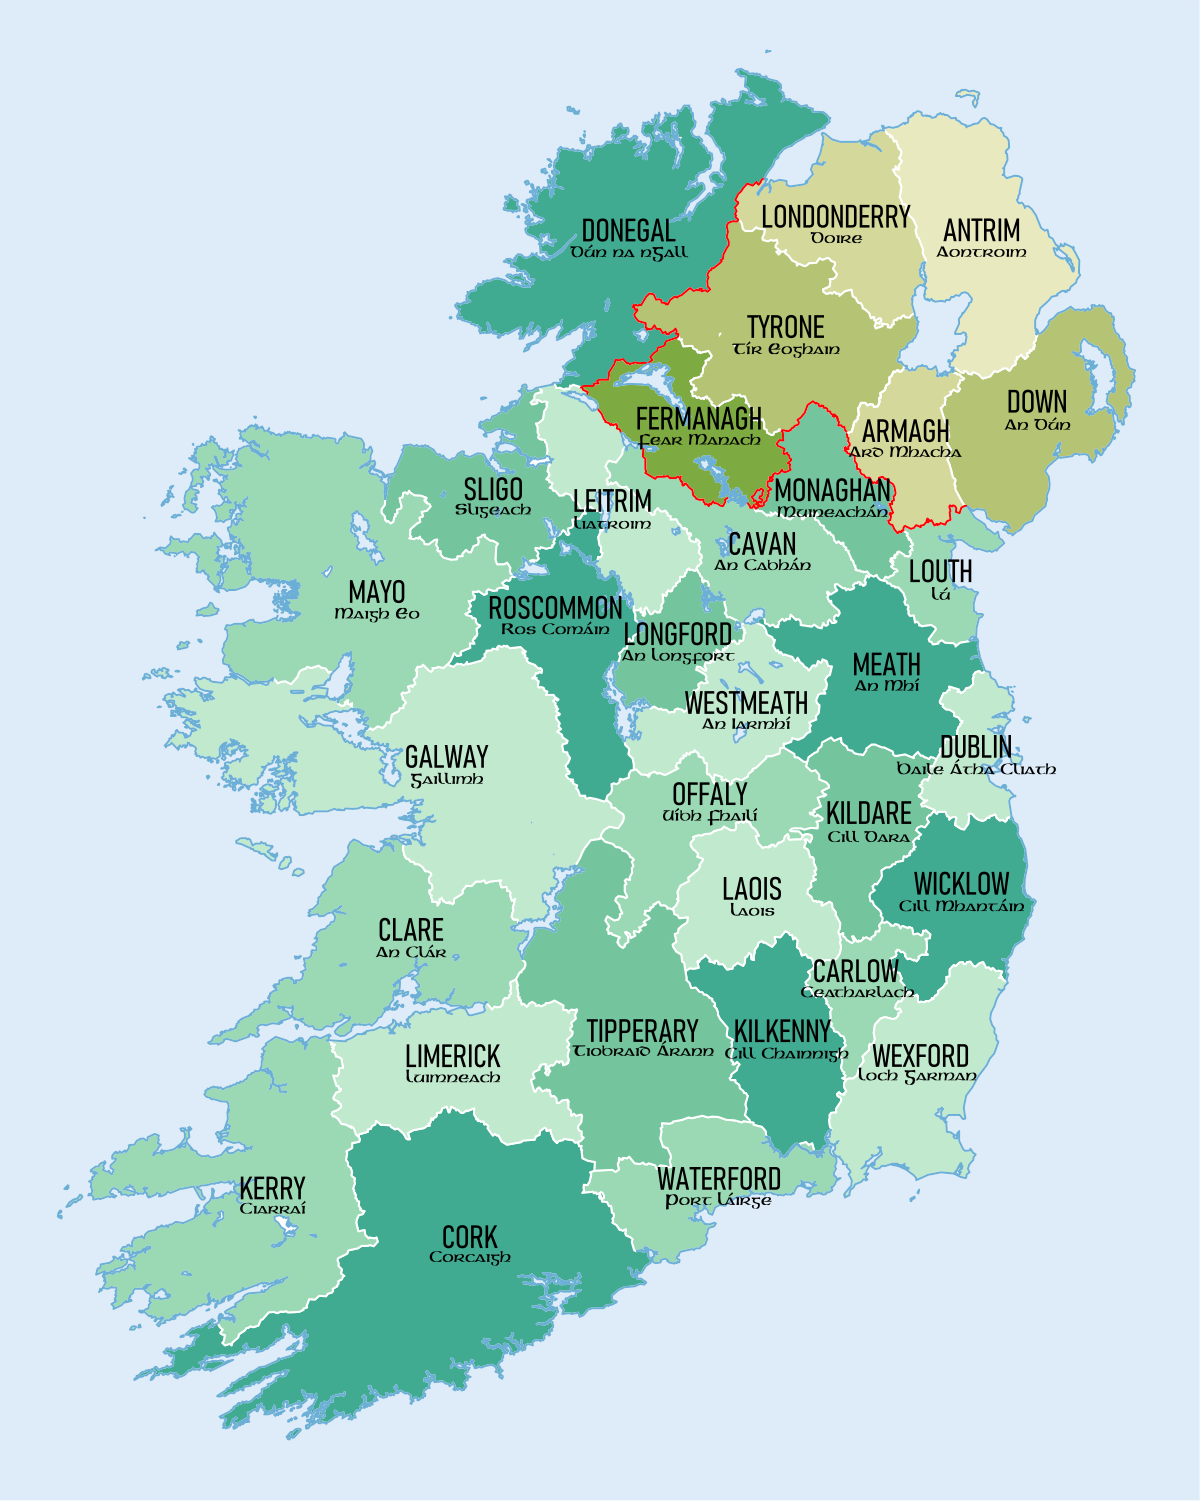
\includegraphics[max width=0.95\textwidth,
        max height=0.54000\textheight]{{Images/ireland}.png}
    \end{center}
    \end{column}
    \end{columns}
}
\end{frame}
\begin{frame}[t]{Round 2 --- Ireland --- \mbox{Answer 3}}
\vspace{-0.5em}
\begin{block}{Question}
What is the name of the famous Irish crystal that takes its name from the city in which it is produced?
\end{block}

\visible<2->{
    \begin{columns}[T,totalwidth=\linewidth]
    \begin{column}{0.32\linewidth}
    \begin{block}{Answer}
    Waterford
    \end{block}
    \end{column}
    \begin{column}{0.65\linewidth}
    \begin{center}
    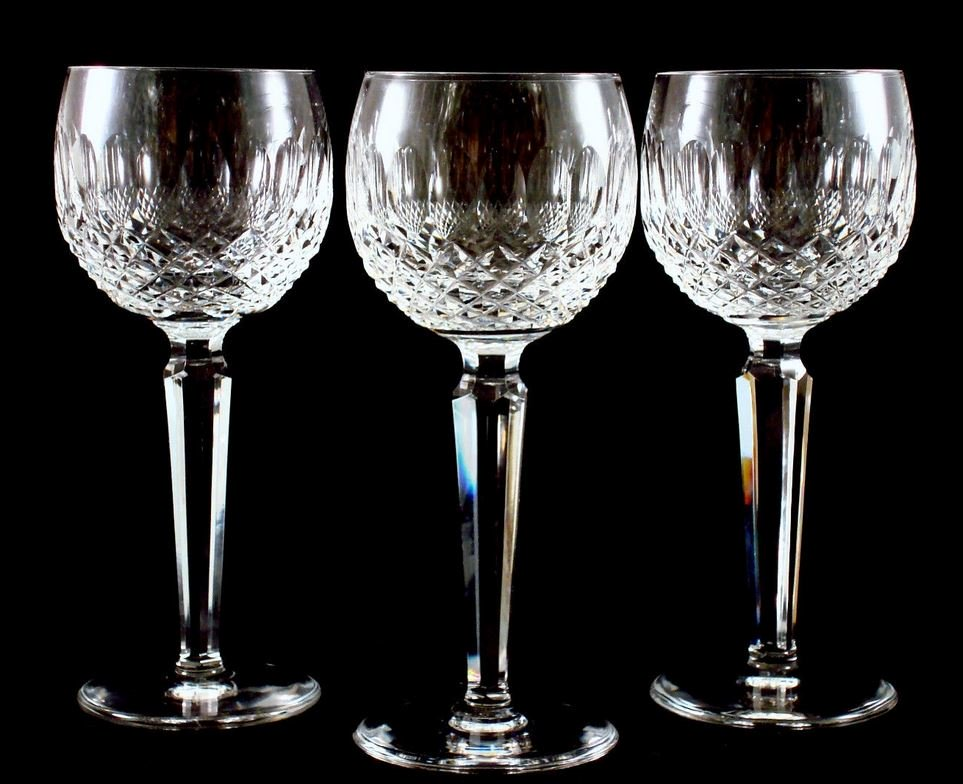
\includegraphics[max width=0.95\textwidth,
        max height=0.50000\textheight]{{Images/waterford}.JPG}
    \end{center}
    \end{column}
    \end{columns}
}
\end{frame}
\begin{frame}[t]{Round 2 --- Ireland --- \mbox{Answer 4}}
\vspace{-0.5em}
\begin{block}{Question}
What is the name of the northernmost peninsula in County Kerry, known for its stunningly beautiful scenery?
\end{block}

\visible<2->{
    \begin{columns}[T,totalwidth=\linewidth]
    \begin{column}{0.32\linewidth}
    \begin{block}{Answer}
    The Dingle Peninsula / The Dingle
    \end{block}
    \end{column}
    \begin{column}{0.65\linewidth}
    \begin{center}
    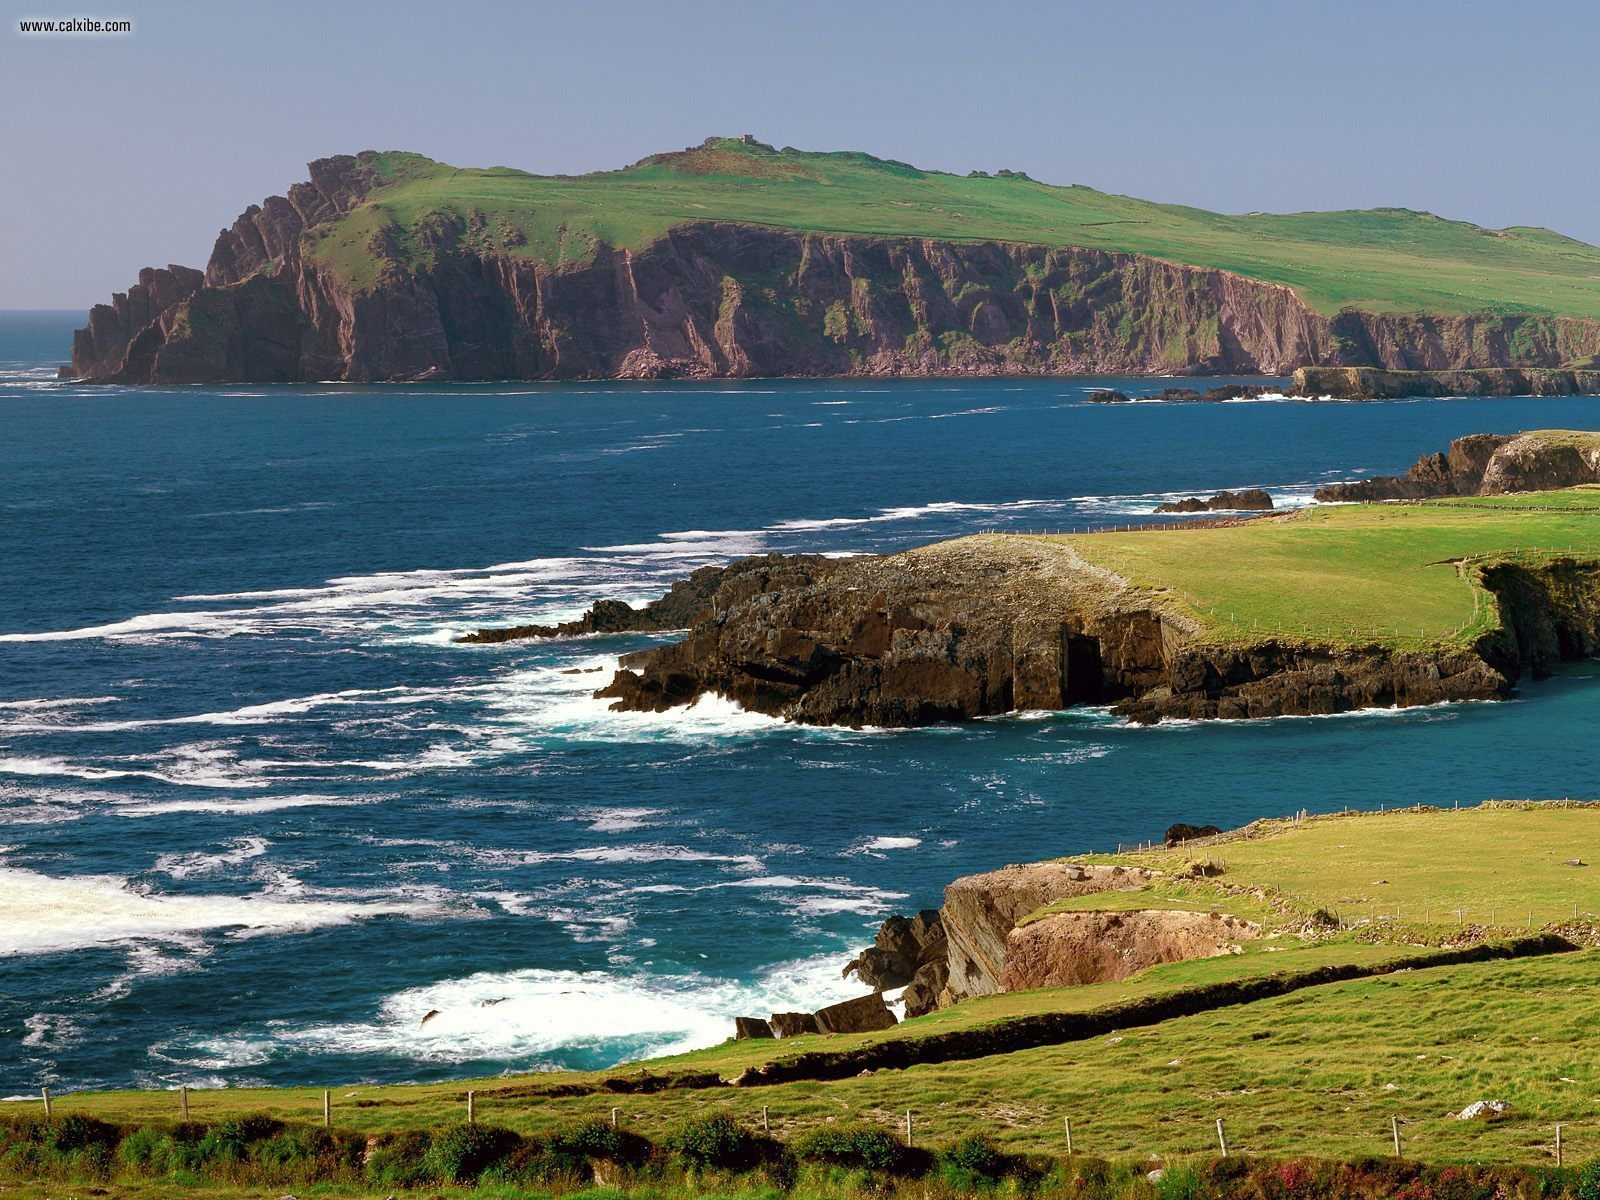
\includegraphics[max width=0.95\textwidth,
        max height=0.50000\textheight]{{Images/dingle}.jpg}
    \end{center}
    \end{column}
    \end{columns}
}
\end{frame}
\begin{frame}[t]{Round 2 --- Ireland --- \mbox{Answer 5}}
\vspace{-0.5em}
\begin{block}{Question}
By population, what is the second largest city in Ireland?
\end{block}

\visible<2->{
    \begin{columns}[T,totalwidth=\linewidth]
    \begin{column}{0.32\linewidth}
    \begin{block}{Answer}
    Cork
    \end{block}
    \end{column}
    \begin{column}{0.65\linewidth}
    \begin{center}
    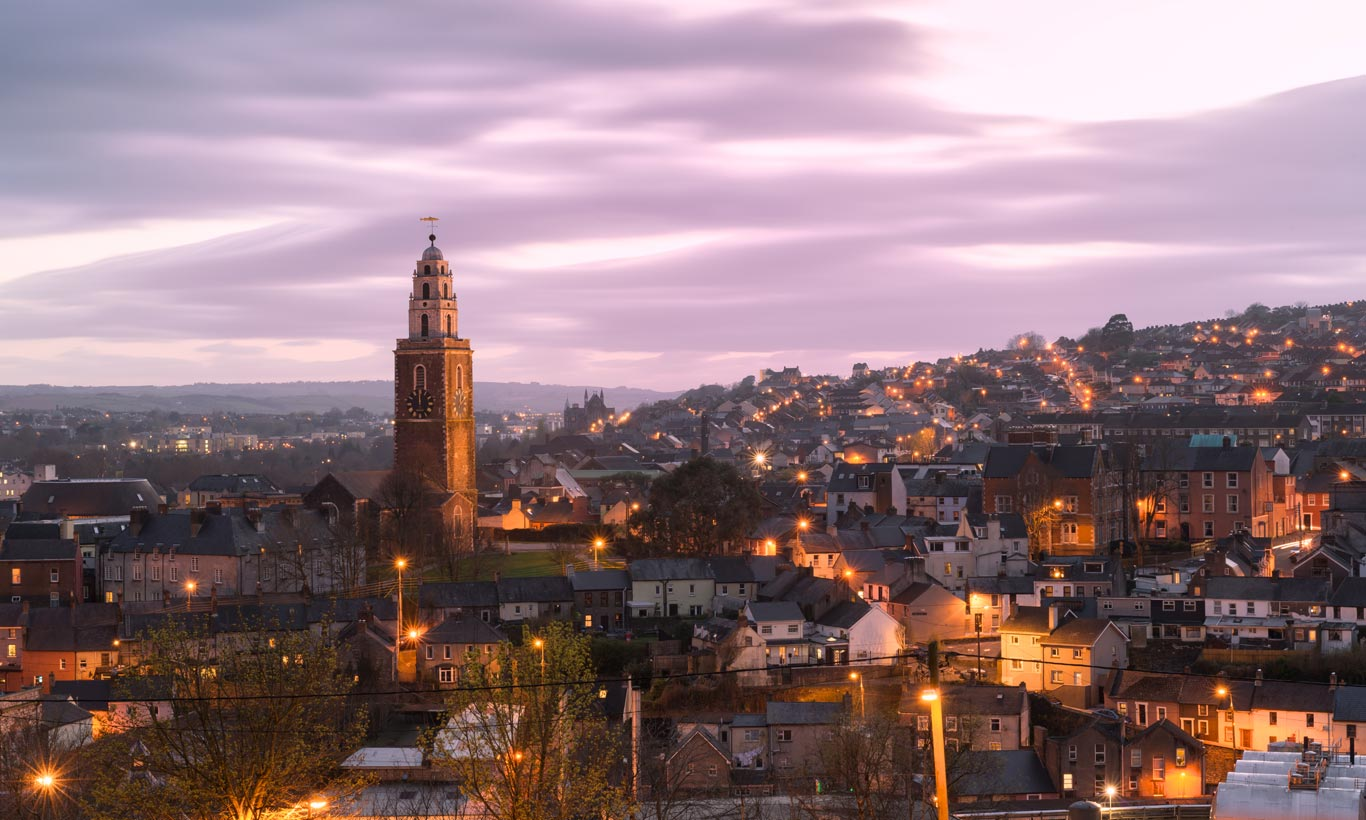
\includegraphics[max width=0.95\textwidth,
        max height=0.54000\textheight]{{Images/cork}.jpg}
    \end{center}
    \end{column}
    \end{columns}
}
\end{frame}
\begin{frame}[t]{Round 2 --- Ireland --- \mbox{Answer 6}}
\vspace{-0.5em}
\begin{block}{Question}
In what year did the Irish win their independence from Great Britain?
\end{block}

\visible<2->{
    \begin{columns}[T,totalwidth=\linewidth]
    \begin{column}{0.32\linewidth}
    \begin{block}{Answer}
    1921
    \end{block}
    \end{column}
    \begin{column}{0.65\linewidth}
    \begin{center}
    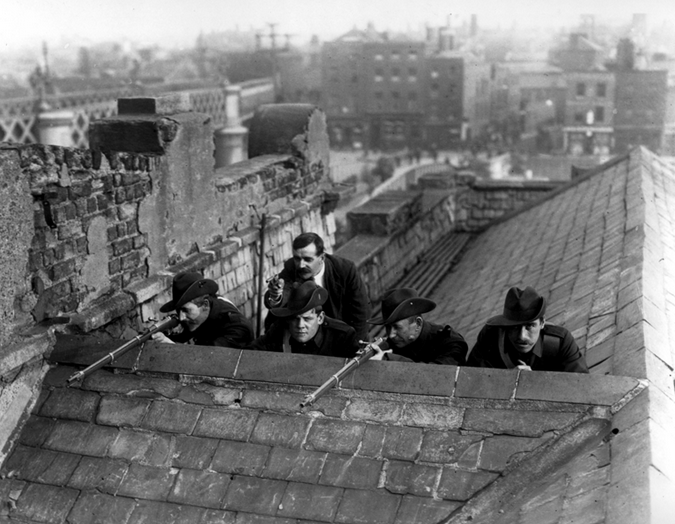
\includegraphics[max width=0.95\textwidth,
        max height=0.54000\textheight]{{Images/irishindependence}.png}
    \end{center}
    \end{column}
    \end{columns}
}
\end{frame}
\begin{frame}[t]{Round 2 --- Ireland --- \mbox{Answer 7}}
\vspace{-0.5em}
\begin{block}{Question}
What  is the name of the Yeats poem that includes the repeated line, ``A terrible beauty is born''?
\end{block}

\visible<2->{
    \begin{columns}[T,totalwidth=\linewidth]
    \begin{column}{0.32\linewidth}
    \begin{block}{Answer}
    ``Easter, 1916''
    \end{block}
    \end{column}
    \begin{column}{0.65\linewidth}
    \begin{center}
    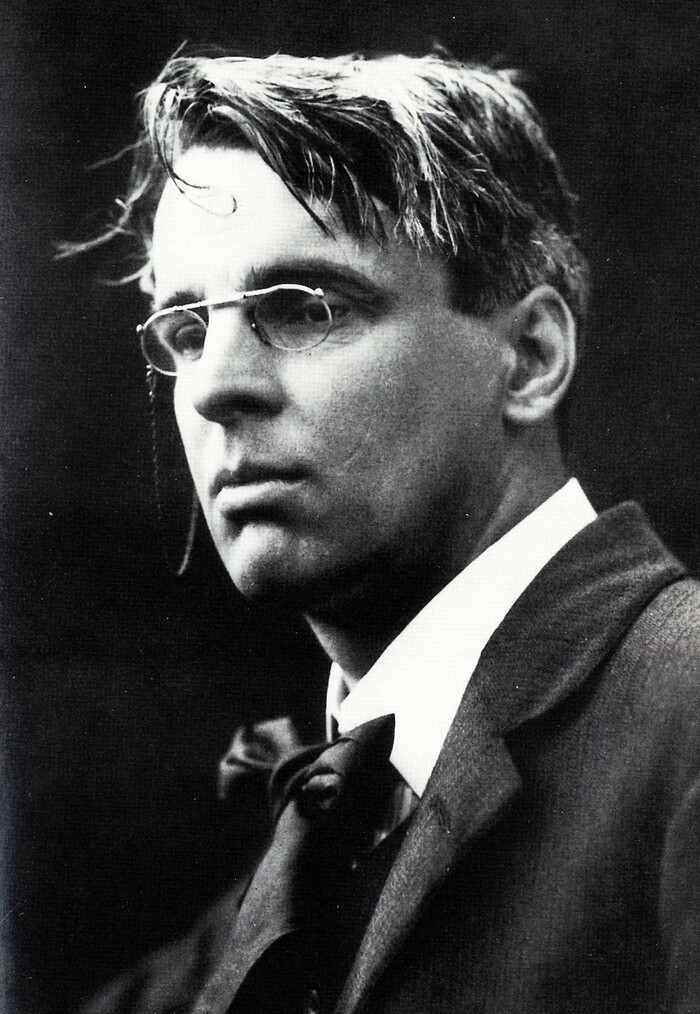
\includegraphics[max width=0.95\textwidth,
        max height=0.54000\textheight]{{Images/yeats}.jpg}
    \end{center}
    \end{column}
    \end{columns}
}
\end{frame}
\begin{frame}[t]{Round 2 --- Ireland --- \mbox{Answer 8}}
\vspace{-0.5em}
\begin{block}{Question}
What famous oratorio, performed annually around the world to this day, had its debut at The Great Music Hall in Dublin during lent in 1742? 
\end{block}

\visible<2->{
    \begin{columns}[T,totalwidth=\linewidth]
    \begin{column}{0.32\linewidth}
    \begin{block}{Answer}
    Messiah / Handel's Messiah, by George Frideric Handel
    \end{block}
    \end{column}
    \begin{column}{0.65\linewidth}
    \begin{center}
    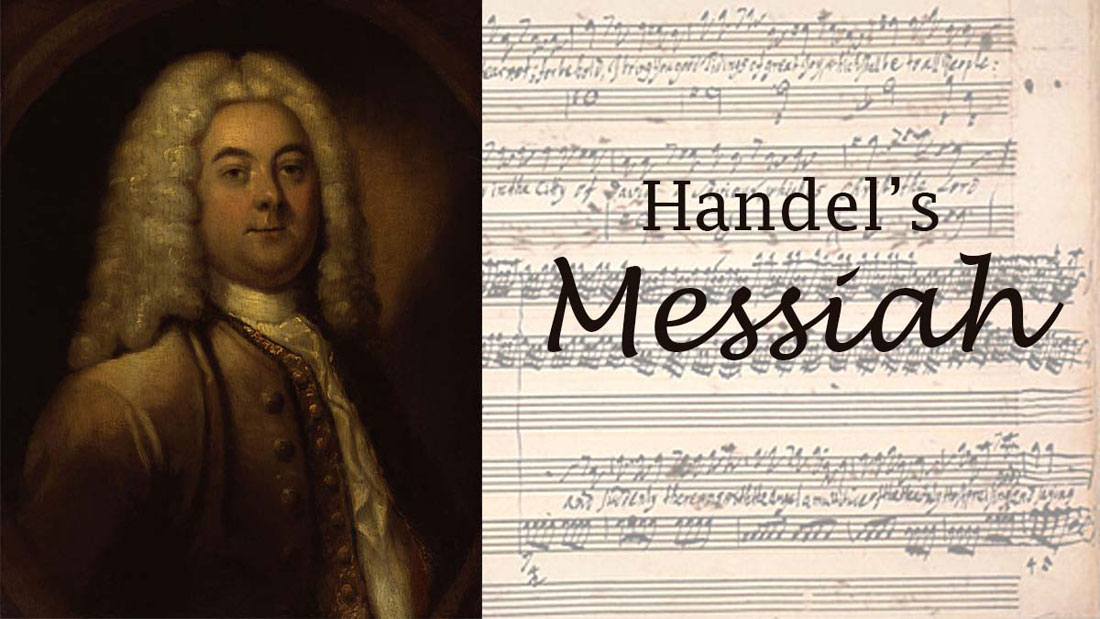
\includegraphics[max width=0.95\textwidth,
        max height=0.50000\textheight]{{Images/handel}.jpg}
    \end{center}
    \end{column}
    \end{columns}
}
\end{frame}
\begin{frame}[t]{Round 2 --- Ireland --- \mbox{Answer 9}}
\vspace{-0.5em}
\begin{block}{Question}
What was Yogi Berra's reported response to being told that Robert Briscoe, the Lord Mayor of Dublin, was Jewish?
\end{block}

\visible<2->{
    \begin{columns}[T,totalwidth=\linewidth]
    \begin{column}{0.32\linewidth}
    \begin{block}{Answer}
    ``Only in America!''
    \end{block}
    \end{column}
    \begin{column}{0.65\linewidth}
    \begin{center}
    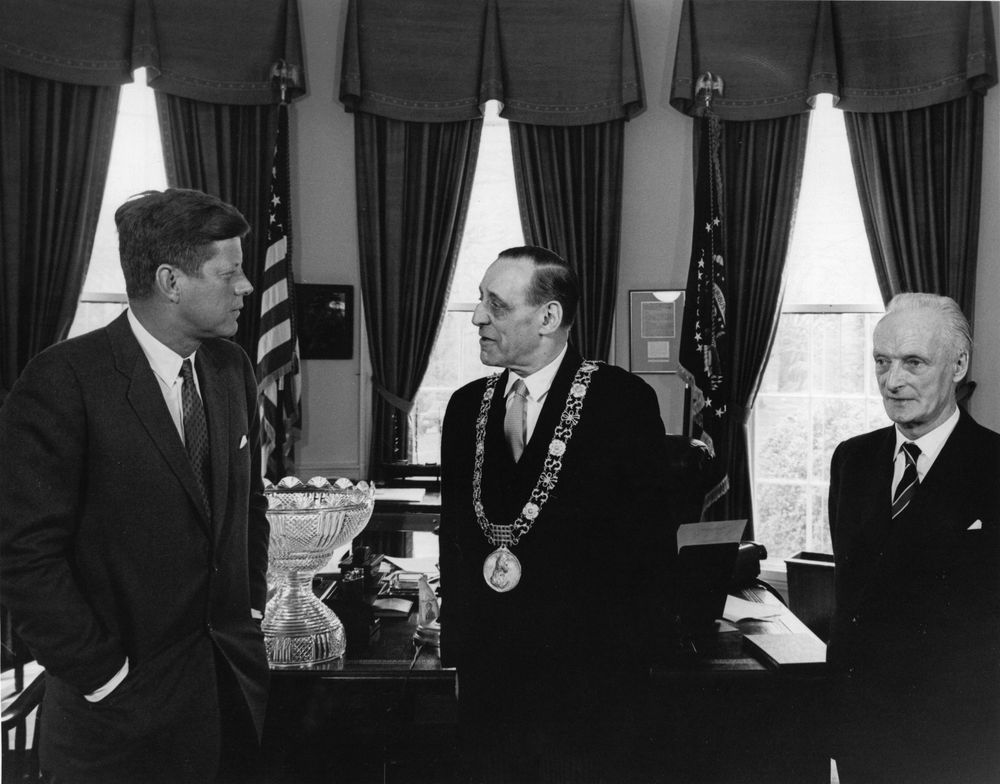
\includegraphics[max width=0.95\textwidth,
        max height=0.50000\textheight]{{Images/briscoe}.jpeg}
    \end{center}
    \end{column}
    \end{columns}
}
\end{frame}
\begin{frame}[t]{Round 2 --- Ireland --- \mbox{Answer 10}}
\vspace{-0.5em}
\begin{block}{Question}
According to legend, what animal did St.\ Patrick drive out of Ireland?
\end{block}

\visible<2->{
    \begin{columns}[T,totalwidth=\linewidth]
    \begin{column}{0.32\linewidth}
    \begin{block}{Answer}
    Snakes
    \end{block}
    \end{column}
    \begin{column}{0.65\linewidth}
    \begin{center}
    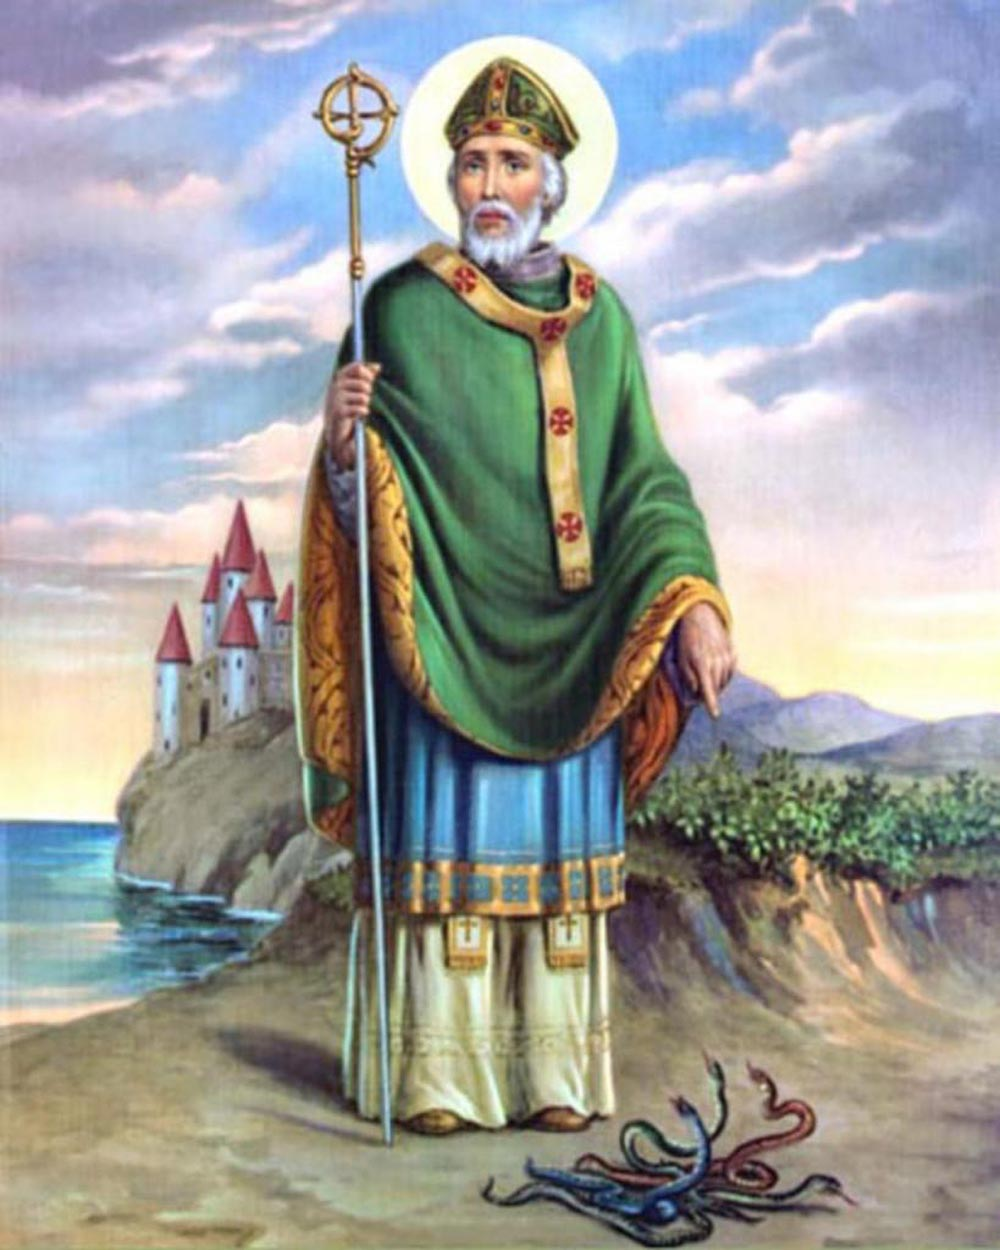
\includegraphics[max width=0.95\textwidth,
        max height=0.54000\textheight]{{Images/stpat}.jpg}
    \end{center}
    \end{column}
    \end{columns}
}
\end{frame}
\def\thisSectionName{Colonial America}
\section{Round 3}
\subsection*{Q1}
\begin{frame}[t]{Round 3 --- Colonial America --- \mbox{Question 1}}
\vspace{-0.5em}
\begin{block}{Question}
The 16\textsuperscript{th} century settlement known as the ``Lost Colony'', whose population mysteriously disappeared, was situated on which island in North Carolina?
\end{block}
\end{frame}
\subsection*{Q2}
\begin{frame}[t]{Round 3 --- Colonial America --- \mbox{Question 2}}
\vspace{-0.5em}
\begin{block}{Question}
What was the name of the first permanent English settlement in America?
\end{block}
\end{frame}
\subsection*{Q3}
\begin{frame}[t]{Round 3 --- Colonial America --- \mbox{Question 3}}
\vspace{-0.5em}
\begin{block}{Question}
What was the name of Pocahontas' husband?
\end{block}
\end{frame}
\subsection*{Q4}
\begin{frame}[t]{Round 3 --- Colonial America --- \mbox{Question 4}}
\vspace{-0.5em}
\begin{block}{Question}
In perhaps the first recorded instance of American exceptionalism, John Winthrop, one of the founders of the Massachusetts Bay Colony, used what Biblical phrase to describe the prominence their colony would have in the world?
\end{block}
\end{frame}
\subsection*{Q5}
\begin{frame}[t]{Round 3 --- Colonial America --- \mbox{Question 5}}
\vspace{-0.5em}
\begin{block}{Question}
Which colony, founded in 1635 by a Puritan dissident, was the first to grant religious freedom to its inhabitants?
\end{block}
\end{frame}
\subsection*{Q6}
\begin{frame}[t]{Round 3 --- Colonial America --- \mbox{Question 6}}
\vspace{-0.5em}
\begin{block}{Question}
Which Revolutionary War hero, who was executed by the British after being captured during a spy mission, said as his last words, ``I only regret that I have but one life to lose for my country''?
\end{block}
\end{frame}
\subsection*{Q7}
\begin{frame}[t]{Round 3 --- Colonial America --- \mbox{Question 7}}
\vspace{-0.5em}
\begin{block}{Question}
Which religious group in colonial America published the first argument in favor of the abolition of slavery?
\end{block}
\end{frame}
\subsection*{Q8}
\begin{frame}[t]{Round 3 --- Colonial America --- \mbox{Question 8}}
\vspace{-0.5em}
\begin{block}{Question}
In what year did the Boston Tea Party occur?
\end{block}
\end{frame}
\subsection*{Q9}
\begin{frame}[t]{Round 3 --- Colonial America --- \mbox{Question 9}}
\vspace{-0.5em}
\begin{block}{Question}
The leading judge in the Salem Witch Trials was an ancestor of a famous 19\textsuperscript{th} century American writer. What was the writer's name?
\end{block}
\end{frame}
\subsection*{Q10}
\begin{frame}[t]{Round 3 --- Colonial America --- \mbox{Question 10}}
\vspace{-0.5em}
\begin{columns}[T,totalwidth=\linewidth]
\begin{column}{0.32\linewidth}
\begin{block}{Question}
Which founding father published the political cartoon pictured here in the \emph{Pennsylvania Gazette} in 1754?
\end{block}
\end{column}
\begin{column}{0.65\linewidth}
\begin{center}
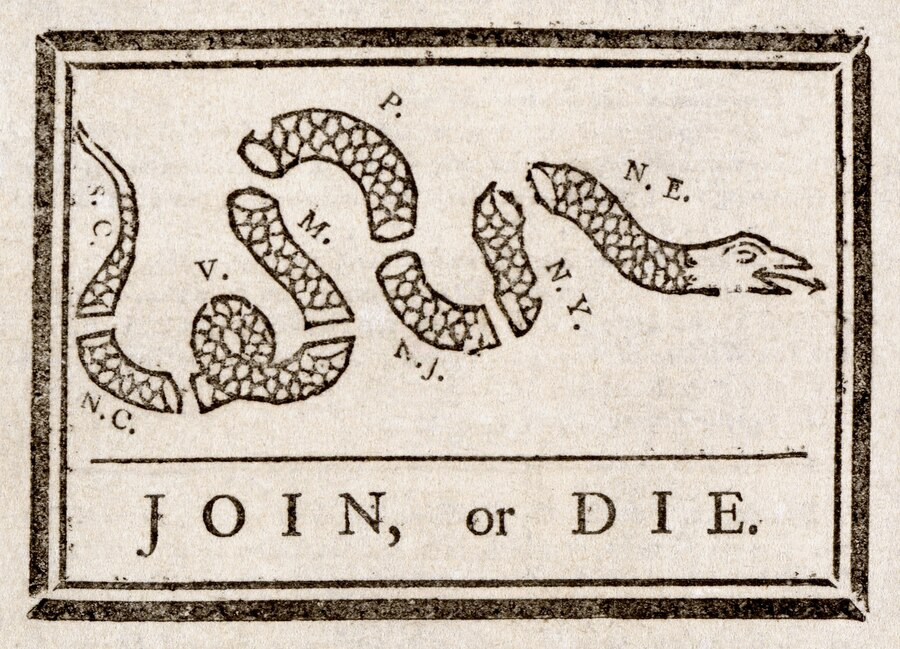
\includegraphics[max width=0.95\textwidth,max height=0.7\textheight]{{Images/joinordie}.jpg}
\end{center}
\end{column}
\end{columns}
\end{frame}
\subsection{Answers}
\begin{frame}[t]{Round 3 --- Colonial America --- \mbox{Answer 1}}
\vspace{-0.5em}
\begin{block}{Question}
The 16\textsuperscript{th} century settlement known as the ``Lost Colony'', whose population mysteriously disappeared, was situated on which island in North Carolina?
\end{block}

\visible<2->{
    \begin{columns}[T,totalwidth=\linewidth]
    \begin{column}{0.32\linewidth}
    \begin{block}{Answer}
    Roanoke
    \end{block}
    \end{column}
    \begin{column}{0.65\linewidth}
    \begin{center}
    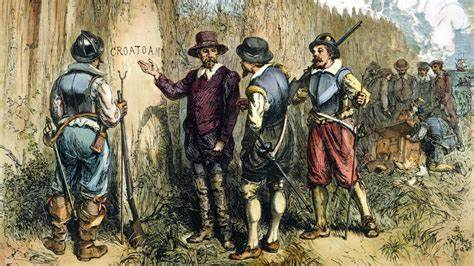
\includegraphics[max width=0.95\textwidth,
        max height=0.46000\textheight]{{Images/roanoke}.jpeg}
    \end{center}
    \end{column}
    \end{columns}
}
\end{frame}
\begin{frame}[t]{Round 3 --- Colonial America --- \mbox{Answer 2}}
\vspace{-0.5em}
\begin{block}{Question}
What was the name of the first permanent English settlement in America?
\end{block}

\visible<2->{
    \begin{columns}[T,totalwidth=\linewidth]
    \begin{column}{0.32\linewidth}
    \begin{block}{Answer}
    Jamestown, Virginia
    \end{block}
    \end{column}
    \begin{column}{0.65\linewidth}
    \begin{center}
    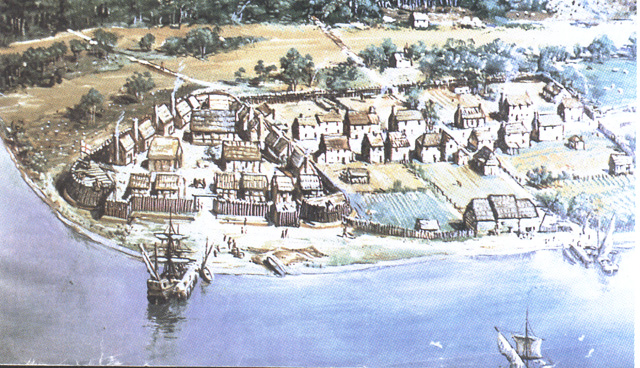
\includegraphics[max width=0.95\textwidth,
        max height=0.54000\textheight]{{Images/jamestownfort}.jpg}
    \end{center}
    \end{column}
    \end{columns}
}
\end{frame}
\begin{frame}[t]{Round 3 --- Colonial America --- \mbox{Answer 3}}
\vspace{-0.5em}
\begin{block}{Question}
What was the name of Pocahontas' husband?
\end{block}

\visible<2->{
    \begin{columns}[T,totalwidth=\linewidth]
    \begin{column}{0.32\linewidth}
    \begin{block}{Answer}
    John Rolfe
    \end{block}
    \end{column}
    \begin{column}{0.65\linewidth}
    \begin{center}
    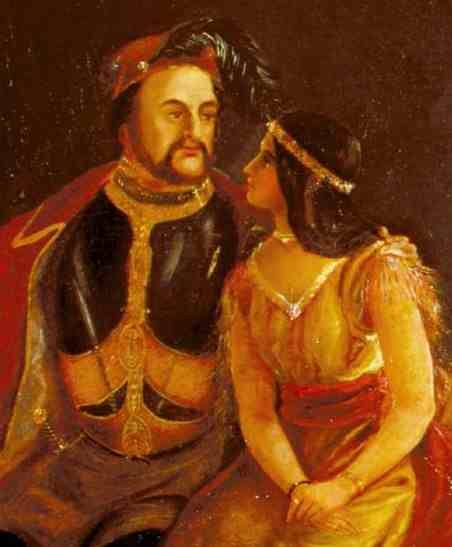
\includegraphics[max width=0.95\textwidth,
        max height=0.58000\textheight]{{Images/rolfe}.jpg}
    \end{center}
    \end{column}
    \end{columns}
}
\end{frame}
\begin{frame}[t]{Round 3 --- Colonial America --- \mbox{Answer 4}}
\vspace{-0.5em}
\begin{block}{Question}
In perhaps the first recorded instance of American exceptionalism, John Winthrop, one of the founders of the Massachusetts Bay Colony, used what Biblical phrase to describe the prominence their colony would have in the world?
\end{block}

\visible<2->{
    \begin{columns}[T,totalwidth=\linewidth]
    \begin{column}{0.32\linewidth}
    \begin{block}{Answer}
    As a ``city upon a hill'' (Matthew 5:14)
    \end{block}
    \end{column}
    \begin{column}{0.65\linewidth}
    \begin{center}
    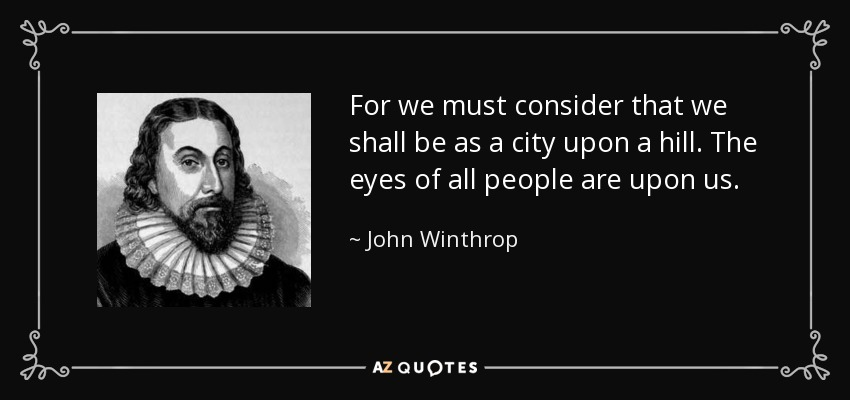
\includegraphics[max width=0.95\textwidth,
        max height=0.42000\textheight]{{Images/winthrop}.jpg}
    \end{center}
    \end{column}
    \end{columns}
}
\end{frame}
\begin{frame}[t]{Round 3 --- Colonial America --- \mbox{Answer 5}}
\vspace{-0.5em}
\begin{block}{Question}
Which colony, founded in 1635 by a Puritan dissident, was the first to grant religious freedom to its inhabitants?
\end{block}

\visible<2->{
    \begin{columns}[T,totalwidth=\linewidth]
    \begin{column}{0.32\linewidth}
    \begin{block}{Answer}
    Rhode Island
    \end{block}
    \end{column}
    \begin{column}{0.65\linewidth}
    \begin{center}
    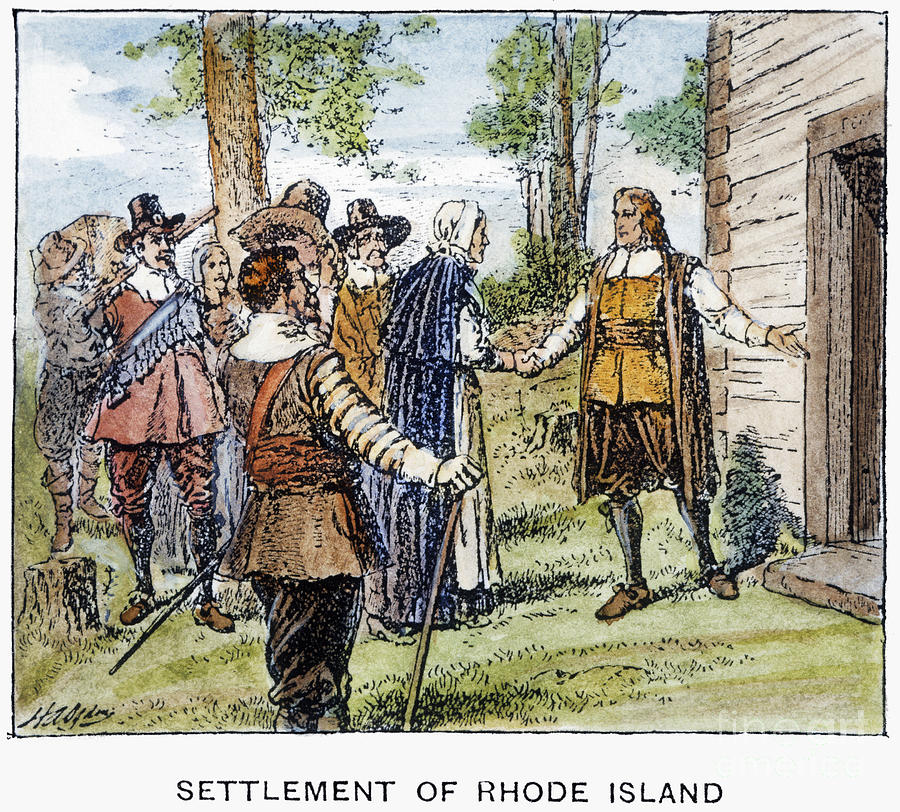
\includegraphics[max width=0.95\textwidth,
        max height=0.50000\textheight]{{Images/rhodeisland}.jpg}
    \end{center}
    \end{column}
    \end{columns}
}
\end{frame}
\begin{frame}[t]{Round 3 --- Colonial America --- \mbox{Answer 6}}
\vspace{-0.5em}
\begin{block}{Question}
Which Revolutionary War hero, who was executed by the British after being captured during a spy mission, said as his last words, ``I only regret that I have but one life to lose for my country''?
\end{block}

\visible<2->{
    \begin{columns}[T,totalwidth=\linewidth]
    \begin{column}{0.32\linewidth}
    \begin{block}{Answer}
    Nathan Hale
    \end{block}
    \end{column}
    \begin{column}{0.65\linewidth}
    \begin{center}
    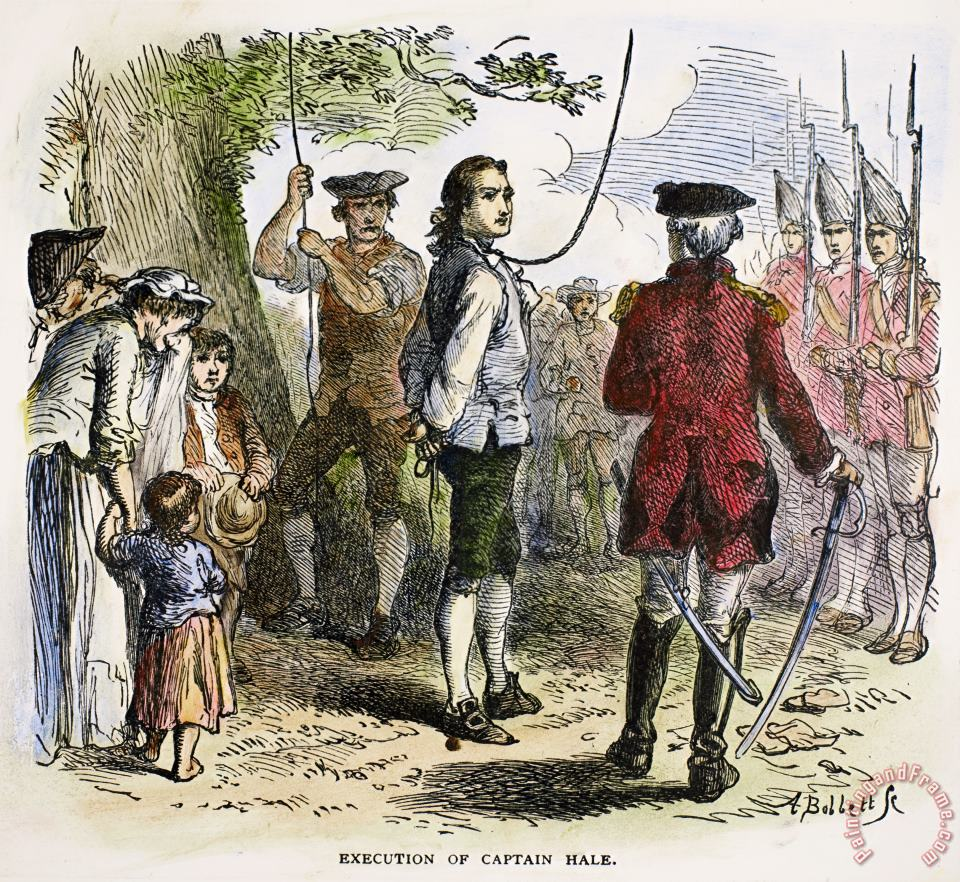
\includegraphics[max width=0.95\textwidth,
        max height=0.46000\textheight]{{Images/nathanhale}.jpg}
    \end{center}
    \end{column}
    \end{columns}
}
\end{frame}
\begin{frame}[t]{Round 3 --- Colonial America --- \mbox{Answer 7}}
\vspace{-0.5em}
\begin{block}{Question}
Which religious group in colonial America published the first argument in favor of the abolition of slavery?
\end{block}

\visible<2->{
    \begin{columns}[T,totalwidth=\linewidth]
    \begin{column}{0.32\linewidth}
    \begin{block}{Answer}
    The Quakers (in 1688)
    \end{block}
    \end{column}
    \begin{column}{0.65\linewidth}
    \begin{center}
    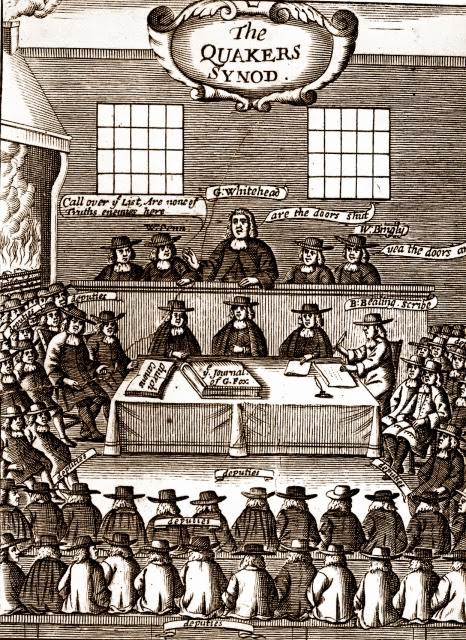
\includegraphics[max width=0.95\textwidth,
        max height=0.50000\textheight]{{Images/quakers}.jpg}
    \end{center}
    \end{column}
    \end{columns}
}
\end{frame}
\begin{frame}[t]{Round 3 --- Colonial America --- \mbox{Answer 8}}
\vspace{-0.5em}
\begin{block}{Question}
In what year did the Boston Tea Party occur?
\end{block}

\visible<2->{
    \begin{columns}[T,totalwidth=\linewidth]
    \begin{column}{0.32\linewidth}
    \begin{block}{Answer}
    1773
    \end{block}
    \end{column}
    \begin{column}{0.65\linewidth}
    \begin{center}
    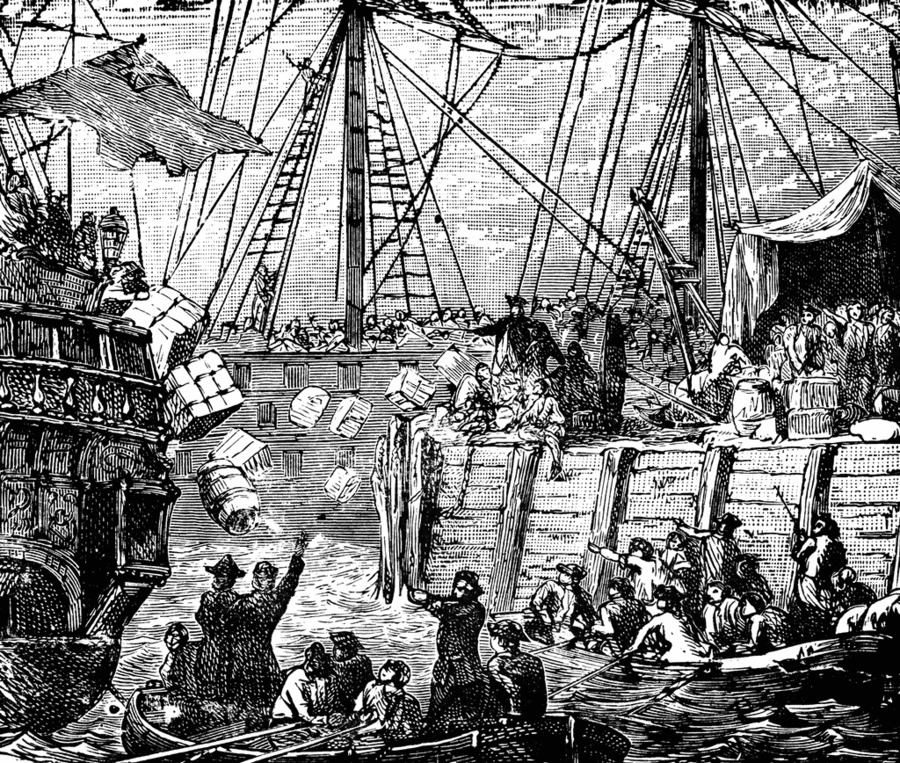
\includegraphics[max width=0.95\textwidth,
        max height=0.58000\textheight]{{Images/btp}.jpg}
    \end{center}
    \end{column}
    \end{columns}
}
\end{frame}
\begin{frame}[t]{Round 3 --- Colonial America --- \mbox{Answer 9}}
\vspace{-0.5em}
\begin{block}{Question}
The leading judge in the Salem Witch Trials was an ancestor of a famous 19\textsuperscript{th} century American writer. What was the writer's name?
\end{block}

\visible<2->{
    \begin{columns}[T,totalwidth=\linewidth]
    \begin{column}{0.65\linewidth}
    \begin{block}{Answer}
    Nathaniel Hawthorne. (His ancestor was John Hathorne.  Hawthorne added the ``w'' to his last name to disassociate himself from his ancestor.)
    \end{block}
    \end{column}
    \begin{column}{0.3\linewidth}
    \begin{center}
    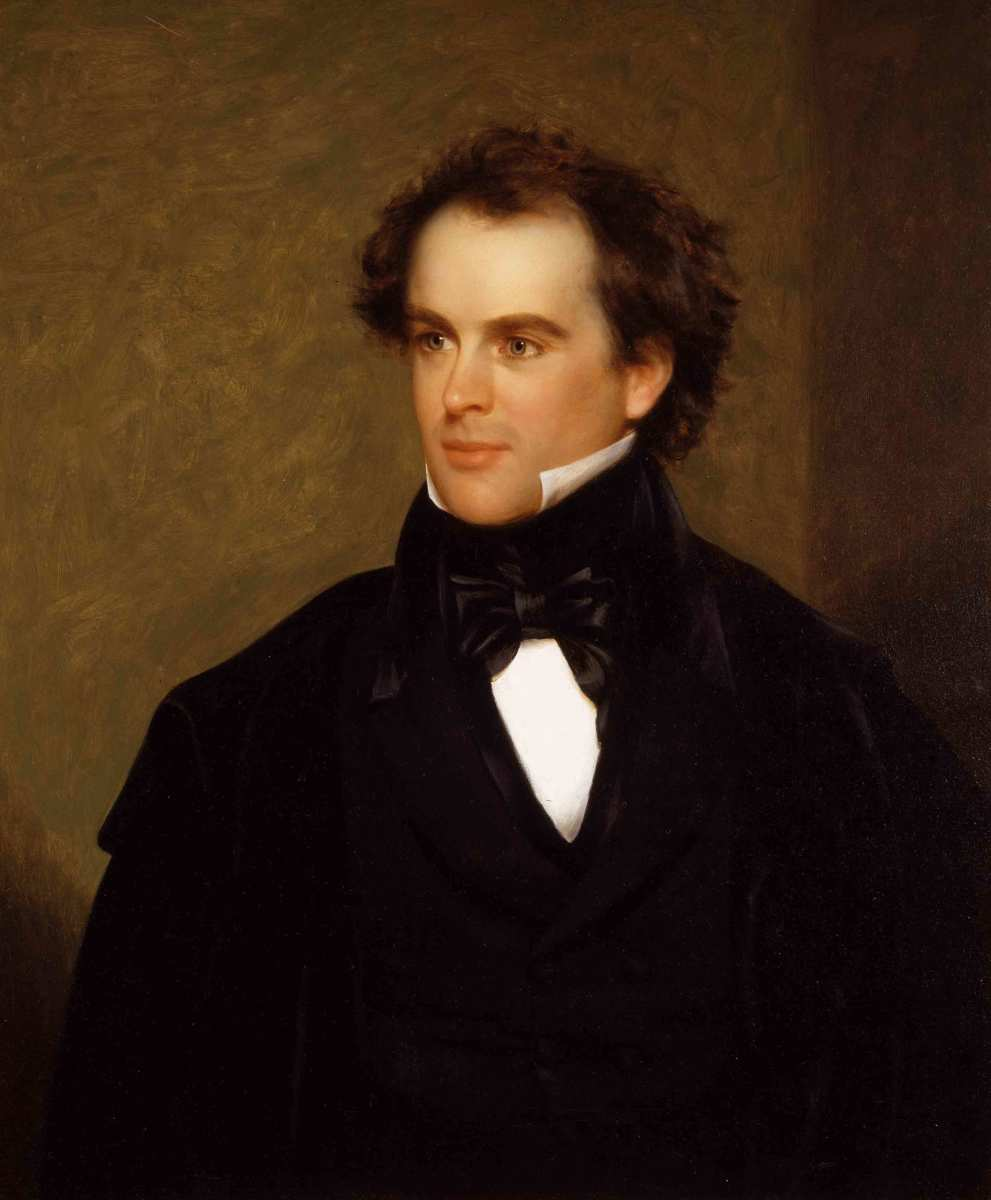
\includegraphics[max width=0.95\textwidth,
        max height=0.50000\textheight]{{Images/hawthorne}.jpg}
    \end{center}
    \end{column}
    \end{columns}
}
\end{frame}
\begin{frame}[t]{Round 3 --- Colonial America --- \mbox{Answer 10}}
\vspace{-0.5em}
\begin{columns}[T,totalwidth=\linewidth]
\begin{column}{0.32\linewidth}
\begin{block}{Question}
Which founding father published the political cartoon pictured here in the \emph{Pennsylvania Gazette} in 1754?
\end{block}
\visible<2->{
    \begin{block}{Answer}
    Benjamin Franklin
    \end{block}
}
\end{column}
\begin{column}{0.65\linewidth}
\begin{center}
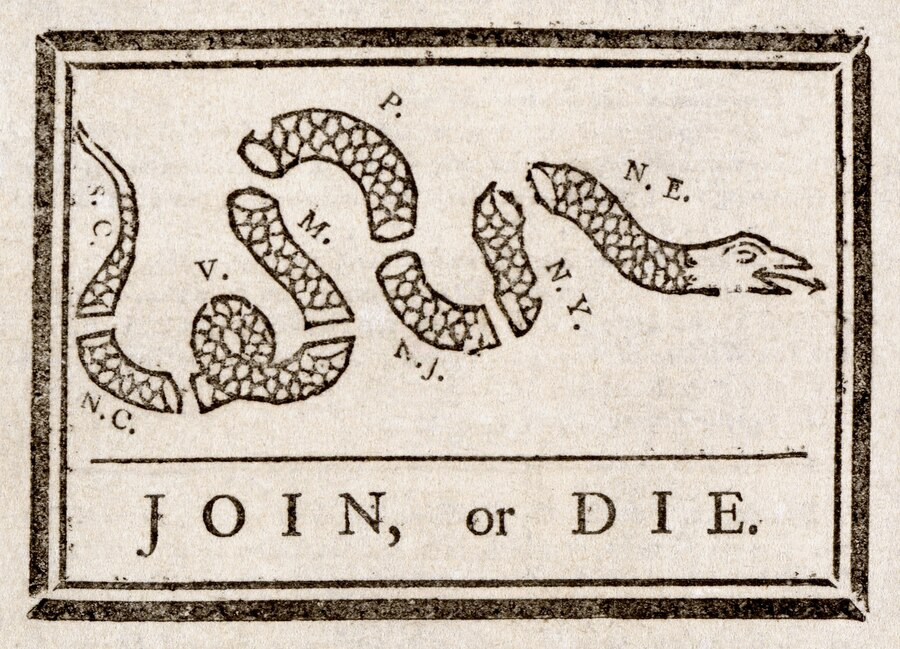
\includegraphics[max width=0.95\textwidth,max height=0.7\textheight]{{Images/joinordie}.jpg}
\end{center}
\end{column}
\end{columns}
\end{frame}
\def\thisSectionName{Famous Ships and Boats}
\section{Round 4}
\subsection*{Q1}
\begin{frame}[t]{Round 4 --- Famous Ships and Boats --- \mbox{Question 1}}
\vspace{-0.5em}
\begin{block}{Question}
What was the alpha-numeric designation of the boat that was under the command of Navy Lt. JG John F.\@  Kennedy when it was rammed by a Japanese destroyer during WWII\@?
\end{block}
\end{frame}
\subsection*{Q2}
\begin{frame}[t]{Round 4 --- Famous Ships and Boats --- \mbox{Question 2}}
\vspace{-0.5em}
\begin{block}{Question}
Name either of the Titanic's sister ships.
\end{block}
\end{frame}
\subsection*{Q3}
\begin{frame}[t]{Round 4 --- Famous Ships and Boats --- \mbox{Question 3}}
\vspace{-0.5em}
\begin{block}{Question}
What were the names of Columbus' ships? (We need them all.)
\end{block}
\end{frame}
\subsection*{Q4}
\begin{frame}[t]{Round 4 --- Famous Ships and Boats --- \mbox{Question 4}}
\vspace{-0.5em}
\begin{block}{Question}
What ship is known by the name ``Old Ironsides''?
\end{block}
\end{frame}
\subsection*{Q5}
\begin{frame}[t]{Round 4 --- Famous Ships and Boats --- \mbox{Question 5}}
\vspace{-0.5em}
\begin{block}{Question}
What is the name of the Italian liner that sank in 1956 with the loss of 46 lives?
\end{block}
\end{frame}
\subsection*{Q6}
\begin{frame}[t]{Round 4 --- Famous Ships and Boats --- \mbox{Question 6}}
\vspace{-0.5em}
\begin{block}{Question}
What is the name of ship the capsizing of which in  2012 resulted in worldwide condemnation of its captain when he abandoned the ship while passengers and crew were still on board?
\end{block}
\end{frame}
\subsection*{Q7}
\begin{frame}[t]{Round 4 --- Famous Ships and Boats --- \mbox{Question 7}}
\vspace{-0.5em}
\begin{block}{Question}
What is the name of the ship on which Japan formally surrendered to the U.\@S.\@ at the end of WWII\@?
\end{block}
\end{frame}
\subsection*{Q8}
\begin{frame}[t]{Round 4 --- Famous Ships and Boats --- \mbox{Question 8}}
\vspace{-0.5em}
\begin{block}{Question}
What is the name of the  American ship that exploded under mysterious circumstances in Havana harbor in February 1898? 
\end{block}
\end{frame}
\subsection*{Q9}
\begin{frame}[t]{Round 4 --- Famous Ships and Boats --- \mbox{Question 9}}
\vspace{-0.5em}
\begin{block}{Question}
This ship, one of only three American aircraft carriers commissioned before World War II to survive the war, participated in the course of the war in more major actions against Japan than any other United States ship.
\end{block}
\end{frame}
\subsection*{Q10}
\begin{frame}[t]{Round 4 --- Famous Ships and Boats --- \mbox{Question 10}}
\vspace{-0.5em}
\begin{block}{Question}
What was the name of the ship on which Henry Hudson sailed when he explored the river that would someday bear his name?
\end{block}
\end{frame}
\subsection{Answers}
\begin{frame}[t]{Round 4 --- Famous Ships and Boats --- \mbox{Answer 1}}
\vspace{-0.5em}
\begin{block}{Question}
What was the alpha-numeric designation of the boat that was under the command of Navy Lt. JG John F.\@  Kennedy when it was rammed by a Japanese destroyer during WWII\@?
\end{block}

\visible<2->{
    \begin{columns}[T,totalwidth=\linewidth]
    \begin{column}{0.32\linewidth}
    \begin{block}{Answer}
    PT--109
    \end{block}
    \end{column}
    \begin{column}{0.65\linewidth}
    \begin{center}
    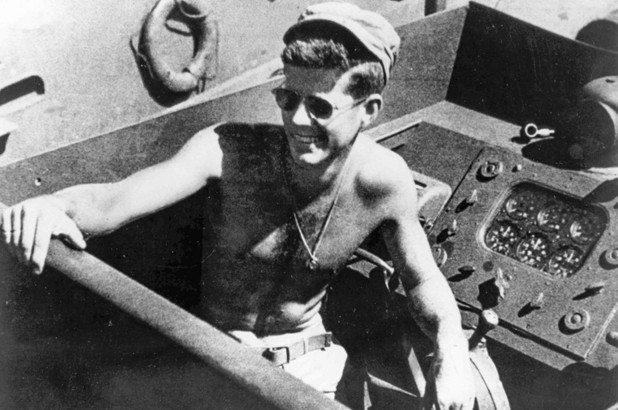
\includegraphics[max width=0.95\textwidth,
        max height=0.46000\textheight]{{Images/jfk}.jpg}
    \end{center}
    \end{column}
    \end{columns}
}
\end{frame}
\begin{frame}[t]{Round 4 --- Famous Ships and Boats --- \mbox{Answer 2}}
\vspace{-0.5em}
\begin{block}{Question}
Name either of the Titanic's sister ships.
\end{block}

\visible<2->{
    \begin{columns}[T,totalwidth=\linewidth]
    \begin{column}{0.32\linewidth}
    \begin{block}{Answer}
    \emph{Britannic} and \emph{Olympic} (you only need one of them)
    \end{block}
    \end{column}
    \begin{column}{0.65\linewidth}
    \begin{center}
    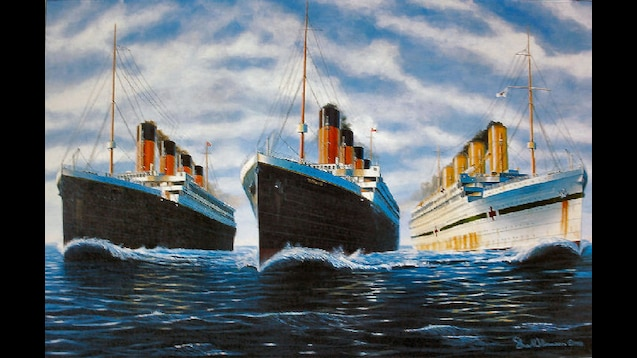
\includegraphics[max width=0.95\textwidth,
        max height=0.58000\textheight]{{Images/titanic}.jpg}
    \end{center}
    \end{column}
    \end{columns}
}
\end{frame}
\begin{frame}[t]{Round 4 --- Famous Ships and Boats --- \mbox{Answer 3}}
\vspace{-0.5em}
\begin{block}{Question}
What were the names of Columbus' ships? (We need them all.)
\end{block}

\visible<2->{
    \begin{columns}[T,totalwidth=\linewidth]
    \begin{column}{0.32\linewidth}
    \begin{block}{Answer}
    The Niña, the Pinta and the Santa Maria
    \end{block}
    \end{column}
    \begin{column}{0.65\linewidth}
    \begin{center}
    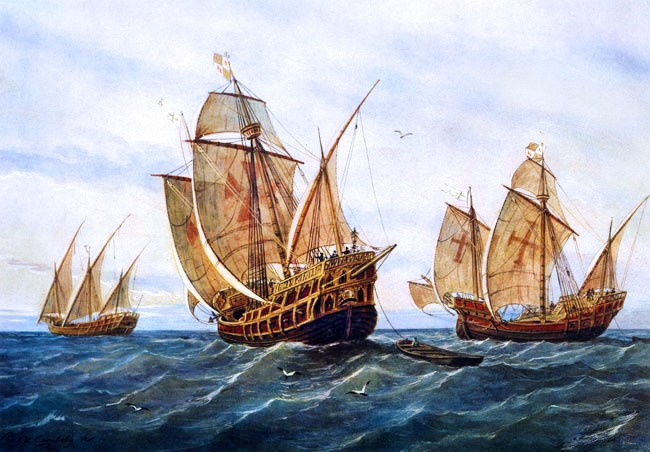
\includegraphics[max width=0.95\textwidth,
        max height=0.54000\textheight]{{Images/columbus}.jpg}
    \end{center}
    \end{column}
    \end{columns}
}
\end{frame}
\begin{frame}[t]{Round 4 --- Famous Ships and Boats --- \mbox{Answer 4}}
\vspace{-0.5em}
\begin{block}{Question}
What ship is known by the name ``Old Ironsides''?
\end{block}

\visible<2->{
    \begin{columns}[T,totalwidth=\linewidth]
    \begin{column}{0.32\linewidth}
    \begin{block}{Answer}
    The U.\@S.\@S.\@ Constitution
    \end{block}
    \end{column}
    \begin{column}{0.65\linewidth}
    \begin{center}
    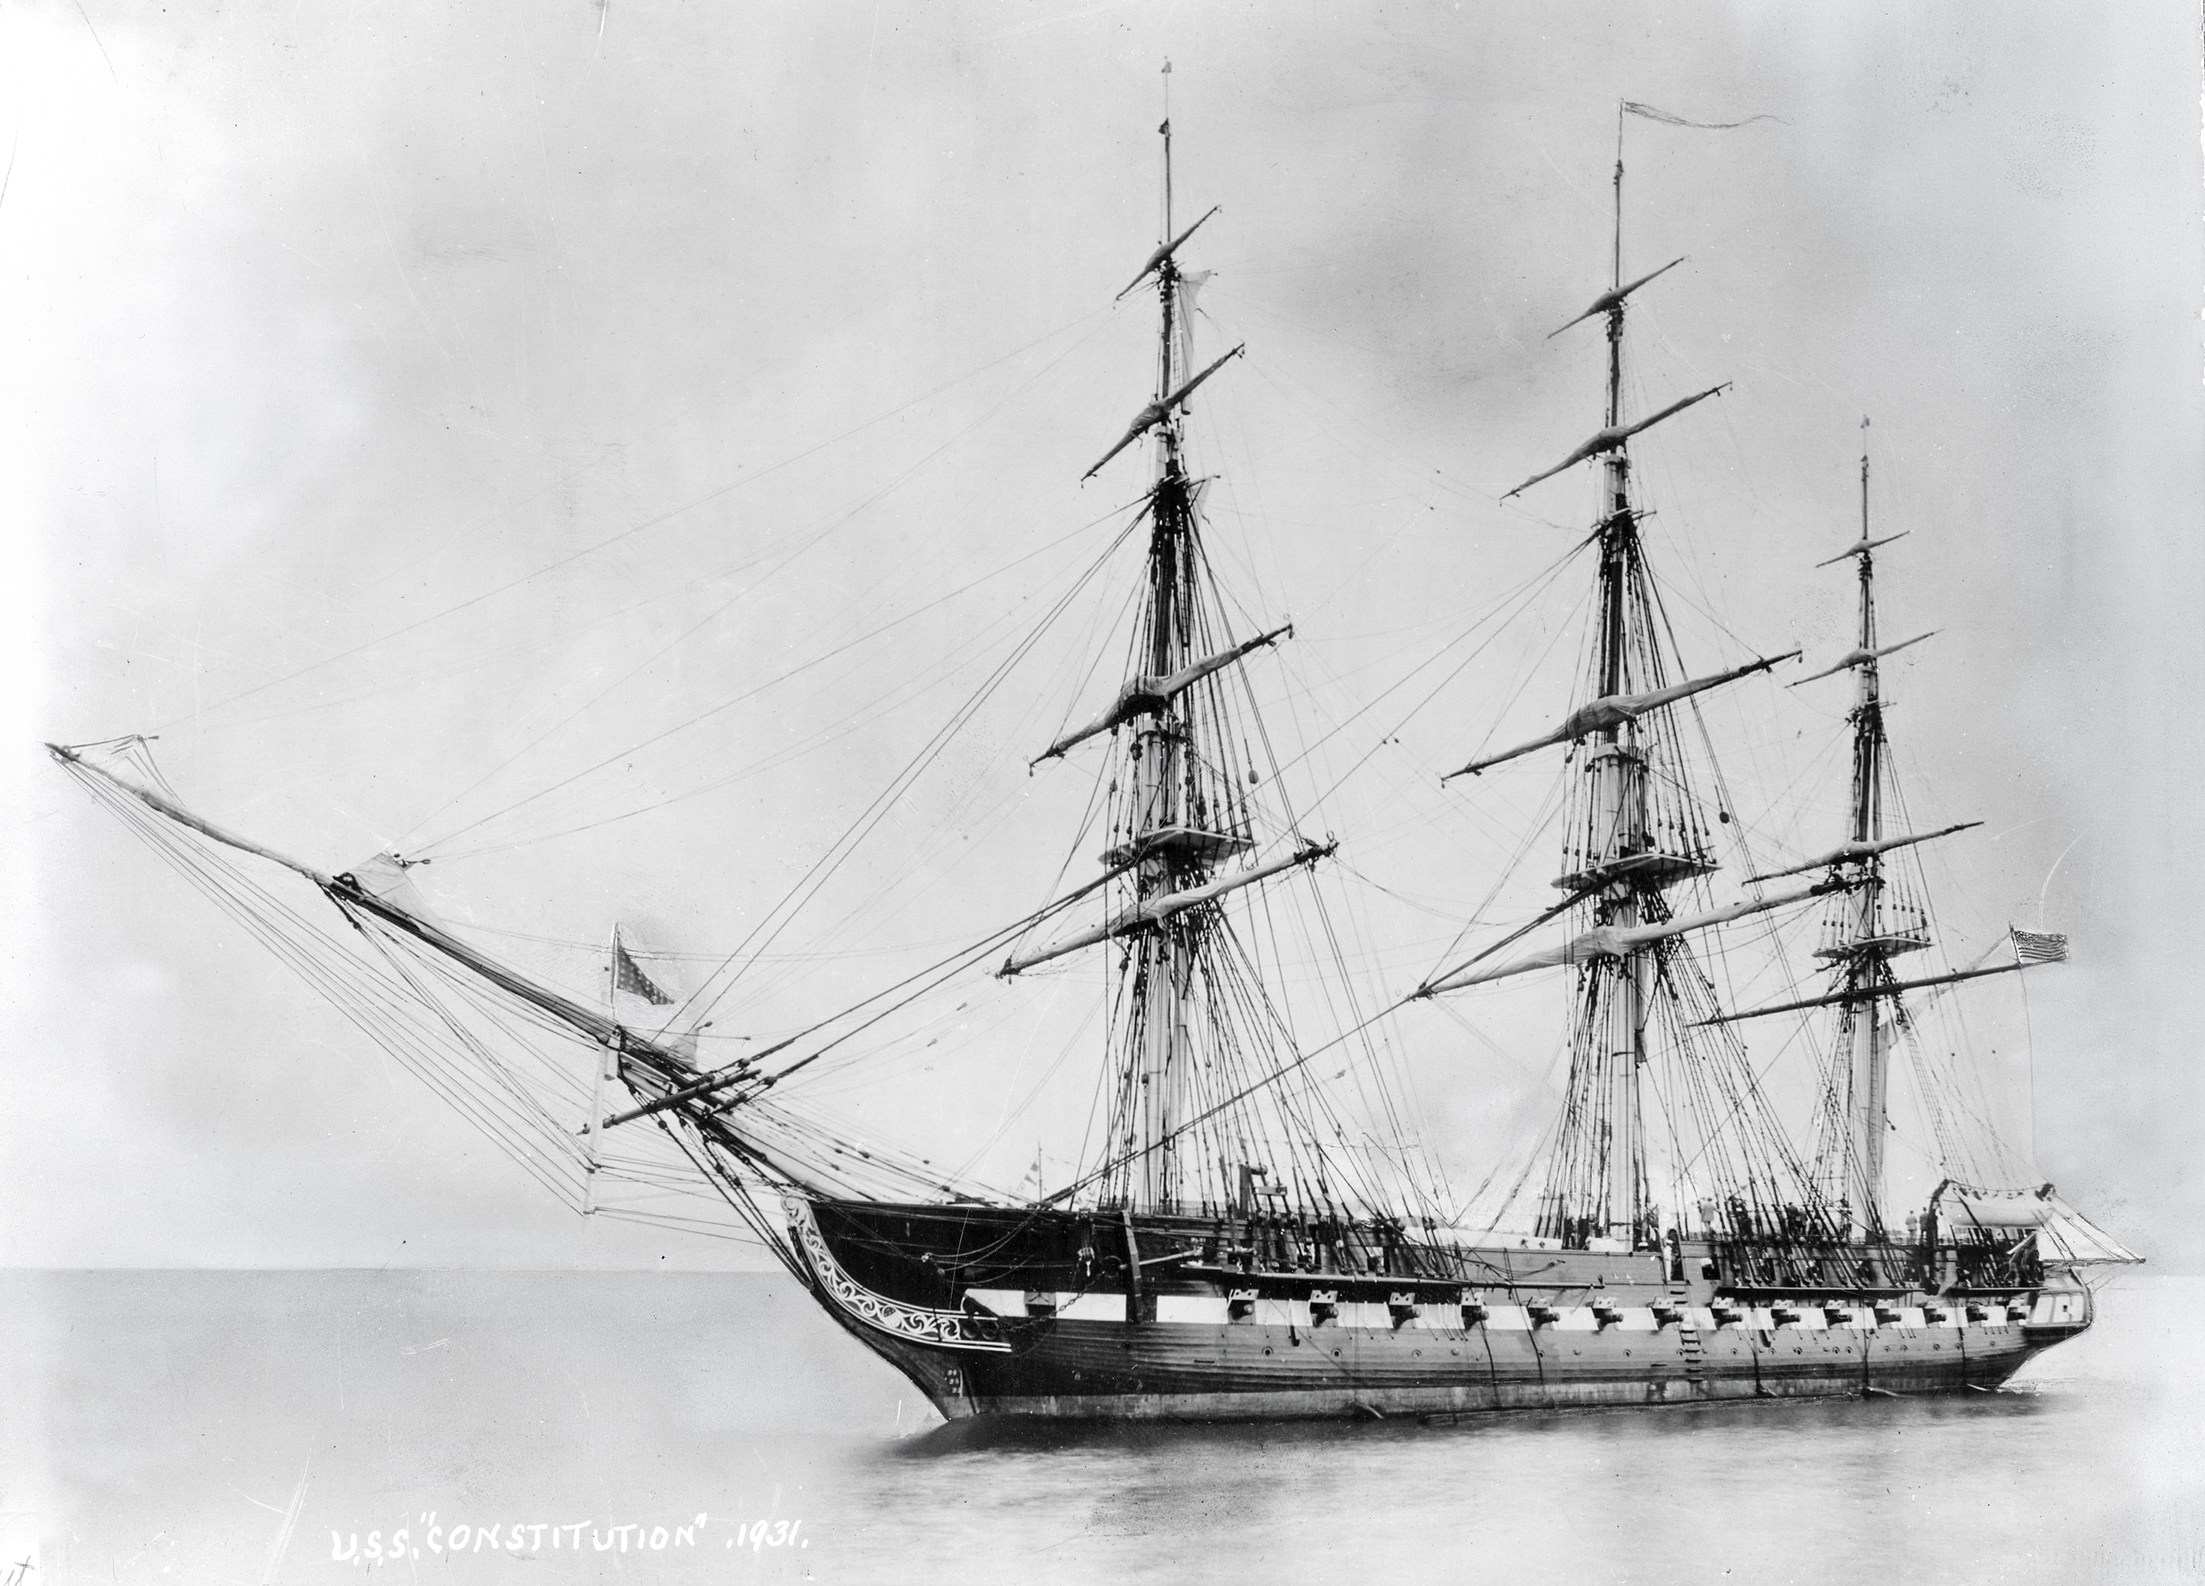
\includegraphics[max width=0.95\textwidth,
        max height=0.58000\textheight]{{Images/constitution}.jpg}
    \end{center}
    \end{column}
    \end{columns}
}
\end{frame}
\begin{frame}[t]{Round 4 --- Famous Ships and Boats --- \mbox{Answer 5}}
\vspace{-0.5em}
\begin{block}{Question}
What is the name of the Italian liner that sank in 1956 with the loss of 46 lives?
\end{block}

\visible<2->{
    \begin{columns}[T,totalwidth=\linewidth]
    \begin{column}{0.32\linewidth}
    \begin{block}{Answer}
    The Andrea Doria (and George did not get the apartment)
    \end{block}
    \end{column}
    \begin{column}{0.65\linewidth}
    \begin{center}
    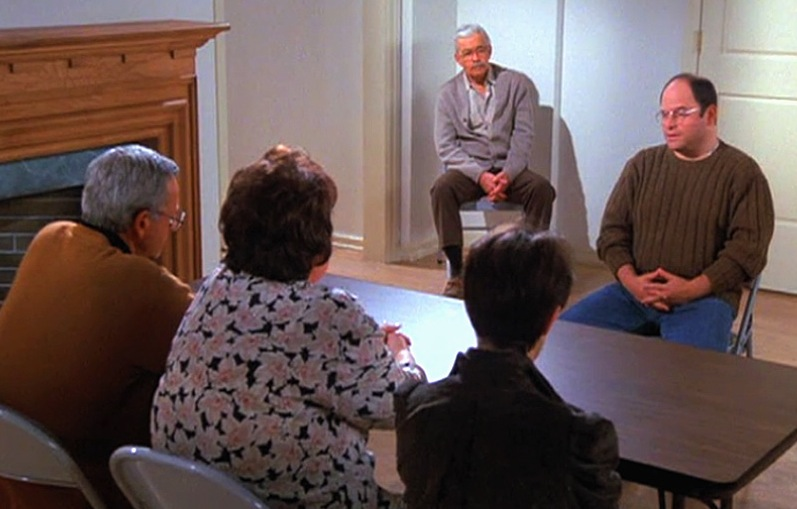
\includegraphics[max width=0.95\textwidth,
        max height=0.54000\textheight]{{Images/andreadoria}.jpg}
    \end{center}
    \end{column}
    \end{columns}
}
\end{frame}
\begin{frame}[t]{Round 4 --- Famous Ships and Boats --- \mbox{Answer 6}}
\vspace{-0.5em}
\begin{block}{Question}
What is the name of ship the capsizing of which in  2012 resulted in worldwide condemnation of its captain when he abandoned the ship while passengers and crew were still on board?
\end{block}

\visible<2->{
    \begin{columns}[T,totalwidth=\linewidth]
    \begin{column}{0.65\linewidth}
    \begin{block}{Answer}
    The Costa Concordia. (The Italian Coast Guard famously radioed the captain, Franceso Schettino, to ``Get the f**k on board'' (``Vada a bordo, cazzo!''))
    \end{block}
    \end{column}
    \begin{column}{0.3\linewidth}
    \begin{center}
    
\includegraphics[max width=0.95\textwidth,
        max height=0.46000\textheight]{{Images/schettino}.png}
    \end{center}
    \end{column}
    \end{columns}
}
\end{frame}
\begin{frame}[t]{Round 4 --- Famous Ships and Boats --- \mbox{Answer 7}}
\vspace{-0.5em}
\begin{block}{Question}
What is the name of the ship on which Japan formally surrendered to the U.\@S.\@ at the end of WWII\@?
\end{block}

\visible<2->{
    \begin{columns}[T,totalwidth=\linewidth]
    \begin{column}{0.32\linewidth}
    \begin{block}{Answer}
    The U.\@S.\@S.\@ Missouri
    \end{block}
    \end{column}
    \begin{column}{0.65\linewidth}
    \begin{center}
    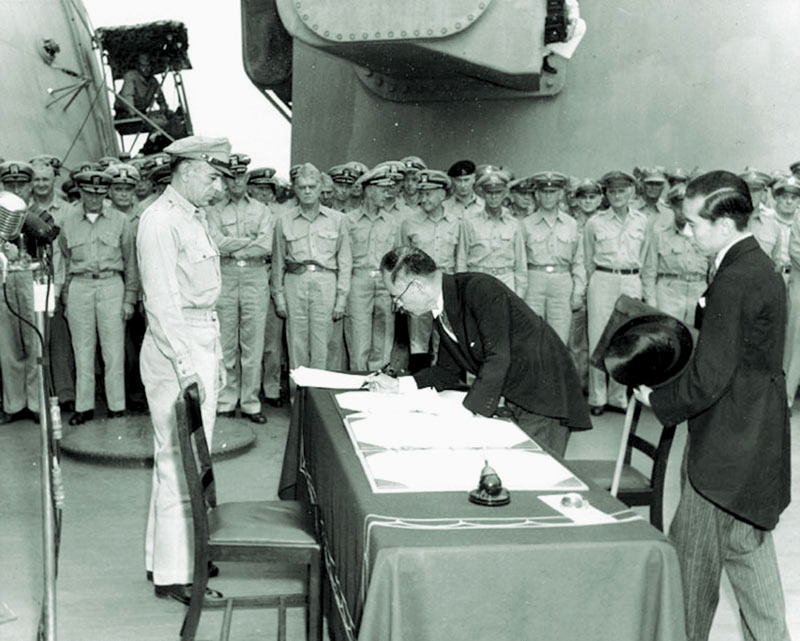
\includegraphics[max width=0.95\textwidth,
        max height=0.50000\textheight]{{Images/missouri}.jpg}
    \end{center}
    \end{column}
    \end{columns}
}
\end{frame}
\begin{frame}[t]{Round 4 --- Famous Ships and Boats --- \mbox{Answer 8}}
\vspace{-0.5em}
\begin{block}{Question}
What is the name of the  American ship that exploded under mysterious circumstances in Havana harbor in February 1898? 
\end{block}

\visible<2->{
    \begin{columns}[T,totalwidth=\linewidth]
    \begin{column}{0.32\linewidth}
    \begin{block}{Answer}
    The U.\@S.\@S.\@ Maine
    \end{block}
    \end{column}
    \begin{column}{0.65\linewidth}
    \begin{center}
    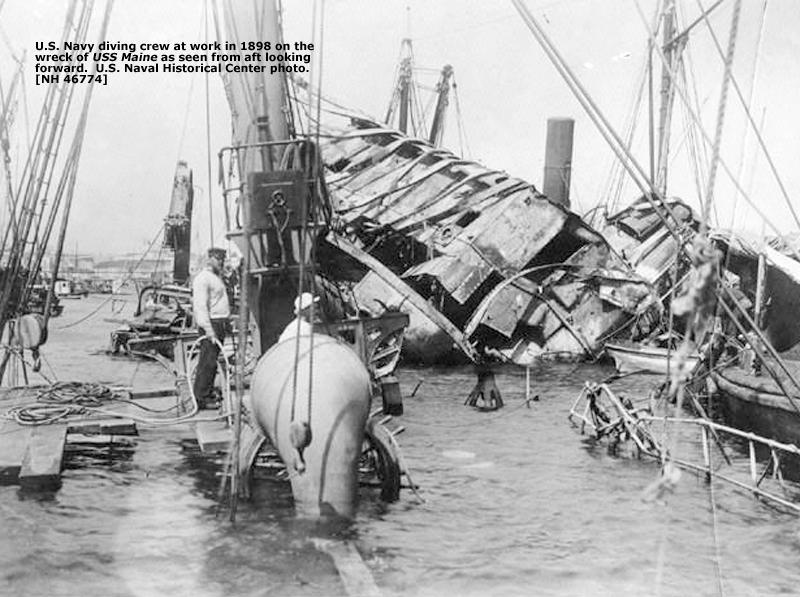
\includegraphics[max width=0.95\textwidth,
        max height=0.50000\textheight]{{Images/mainehulk}.jpg}
    \end{center}
    \end{column}
    \end{columns}
}
\end{frame}
\begin{frame}[t]{Round 4 --- Famous Ships and Boats --- \mbox{Answer 9}}
\vspace{-0.5em}
\begin{block}{Question}
This ship, one of only three American aircraft carriers commissioned before World War II to survive the war, participated in the course of the war in more major actions against Japan than any other United States ship.
\end{block}

\visible<2->{
    \begin{columns}[T,totalwidth=\linewidth]
    \begin{column}{0.32\linewidth}
    \begin{block}{Answer}
    The U.\@S.\@S.\@ Enterprise
    \end{block}
    \end{column}
    \begin{column}{0.65\linewidth}
    \begin{center}
    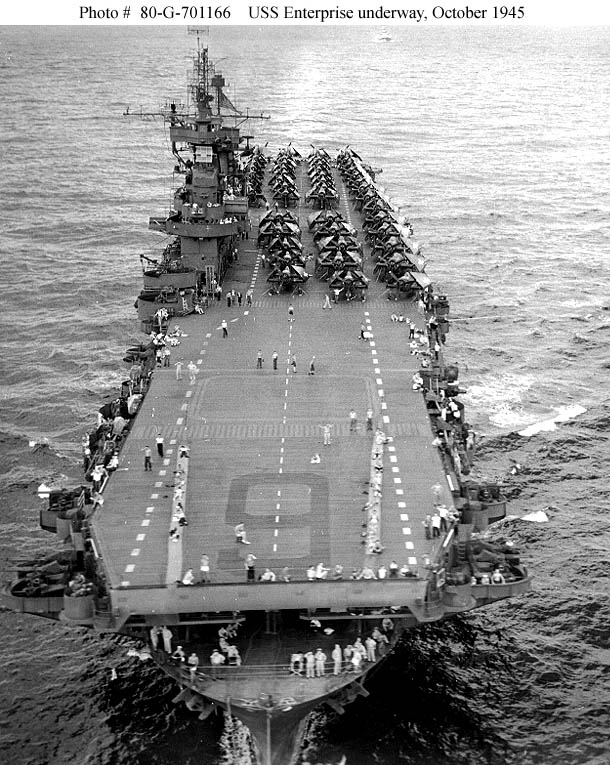
\includegraphics[max width=0.95\textwidth,
        max height=0.42000\textheight]{{Images/enterprise}.jpg}
    \end{center}
    \end{column}
    \end{columns}
}
\end{frame}
\begin{frame}[t]{Round 4 --- Famous Ships and Boats --- \mbox{Answer 10}}
\vspace{-0.5em}
\begin{block}{Question}
What was the name of the ship on which Henry Hudson sailed when he explored the river that would someday bear his name?
\end{block}

\visible<2->{
    \begin{columns}[T,totalwidth=\linewidth]
    \begin{column}{0.32\linewidth}
    \begin{block}{Answer}
    The Half Moon
    \end{block}
    \end{column}
    \begin{column}{0.65\linewidth}
    \begin{center}
    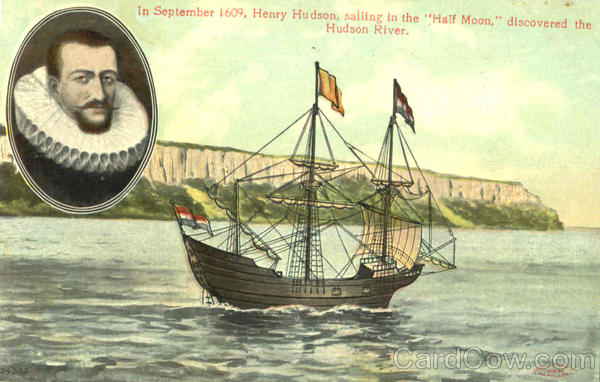
\includegraphics[max width=0.95\textwidth,
        max height=0.50000\textheight]{{Images/hudson}.jpg}
    \end{center}
    \end{column}
    \end{columns}
}
\end{frame}
\def\thisSectionName{Foreign Words and Phrases}
\section{Round 5}
\subsection*{Q1}
\begin{frame}[t]{Round 5 --- Foreign Words and Phrases --- \mbox{Question 1}}
\vspace{-0.5em}
\begin{block}{Question}
Proxime accessit
\end{block}
\end{frame}
\subsection*{Q2}
\begin{frame}[t]{Round 5 --- Foreign Words and Phrases --- \mbox{Question 2}}
\vspace{-0.5em}
\begin{block}{Question}
Persona non grata
\end{block}
\end{frame}
\subsection*{Q3}
\begin{frame}[t]{Round 5 --- Foreign Words and Phrases --- \mbox{Question 3}}
\vspace{-0.5em}
\begin{block}{Question}
Au courant
\end{block}
\end{frame}
\subsection*{Q4}
\begin{frame}[t]{Round 5 --- Foreign Words and Phrases --- \mbox{Question 4}}
\vspace{-0.5em}
\begin{block}{Question}
Beaux arts	
\end{block}
\end{frame}
\subsection*{Q5}
\begin{frame}[t]{Round 5 --- Foreign Words and Phrases --- \mbox{Question 5}}
\vspace{-0.5em}
\begin{block}{Question}
Caveat emptor
\end{block}
\end{frame}
\subsection*{Q6}
\begin{frame}[t]{Round 5 --- Foreign Words and Phrases --- \mbox{Question 6}}
\vspace{-0.5em}
\begin{block}{Question}
In medias res
\end{block}
\end{frame}
\subsection*{Q7}
\begin{frame}[t]{Round 5 --- Foreign Words and Phrases --- \mbox{Question 7}}
\vspace{-0.5em}
\begin{block}{Question}
Unheimlich
\end{block}
\end{frame}
\subsection*{Q8}
\begin{frame}[t]{Round 5 --- Foreign Words and Phrases --- \mbox{Question 8}}
\vspace{-0.5em}
\begin{block}{Question}
Katzenjammer
\end{block}
\end{frame}
\subsection*{Q9}
\begin{frame}[t]{Round 5 --- Foreign Words and Phrases --- \mbox{Question 9}}
\vspace{-0.5em}
\begin{block}{Question}
Plus ça change, plus c'est la même chose.
\end{block}
\end{frame}
\subsection*{Q10}
\begin{frame}[t]{Round 5 --- Foreign Words and Phrases --- \mbox{Question 10}}
\vspace{-0.5em}
\begin{block}{Question}
Sui generis
\end{block}
\end{frame}
\subsection{Answers}
\begin{frame}[t]{Round 5 --- Foreign Words and Phrases --- \mbox{Answer 1}}
\vspace{-0.5em}
\begin{block}{Question}
Proxime accessit
\end{block}

\visible<2->{
    \begin{columns}[T,totalwidth=\linewidth]
    \begin{column}{0.32\linewidth}
    \begin{block}{Answer}
    Person who comes in second / runner up
    \end{block}
    \end{column}
    \begin{column}{0.65\linewidth}
    \begin{center}
    \includegraphics[max width=0.95\textwidth,
        max height=0.58000\textheight]{{Images/proxime}.png}
    \end{center}
    \end{column}
    \end{columns}
}
\end{frame}
\begin{frame}[t]{Round 5 --- Foreign Words and Phrases --- \mbox{Answer 2}}
\vspace{-0.5em}
\begin{block}{Question}
Persona non grata
\end{block}

\visible<2->{
    \begin{columns}[T,totalwidth=\linewidth]
    \begin{column}{0.32\linewidth}
    \begin{block}{Answer}
    An unwelcome or unacceptable person
    \end{block}
    \end{column}
    \begin{column}{0.65\linewidth}
    \begin{center}
    \includegraphics[max width=0.95\textwidth,
        max height=0.58000\textheight]{{Images/nongrata}.png}
    \end{center}
    \end{column}
    \end{columns}
}
\end{frame}
\begin{frame}[t]{Round 5 --- Foreign Words and Phrases --- \mbox{Answer 3}}
\vspace{-0.5em}
\begin{block}{Question}
Au courant
\end{block}

\visible<2->{
    \begin{columns}[T,totalwidth=\linewidth]
    \begin{column}{0.32\linewidth}
    \begin{block}{Answer}
    Up to date / well informed
    \end{block}
    \end{column}
    \begin{column}{0.65\linewidth}
    \begin{center}
    \includegraphics[max width=0.95\textwidth,
        max height=0.58000\textheight]{{Images/aucourant}.jpg}
    \end{center}
    \end{column}
    \end{columns}
}
\end{frame}
\begin{frame}[t]{Round 5 --- Foreign Words and Phrases --- \mbox{Answer 4}}
\vspace{-0.5em}
\begin{block}{Question}
Beaux arts	
\end{block}

\visible<2->{
    \begin{columns}[T,totalwidth=\linewidth]
    \begin{column}{0.32\linewidth}
    \begin{block}{Answer}
    Fine arts
    \end{block}
    \end{column}
    \begin{column}{0.65\linewidth}
    \begin{center}
    \includegraphics[max width=0.95\textwidth,
        max height=0.58000\textheight]{{Images/beauarts}.jpg}
    \end{center}
    \end{column}
    \end{columns}
}
\end{frame}
\begin{frame}[t]{Round 5 --- Foreign Words and Phrases --- \mbox{Answer 5}}
\vspace{-0.5em}
\begin{block}{Question}
Caveat emptor
\end{block}

\visible<2->{
    \begin{columns}[T,totalwidth=\linewidth]
    \begin{column}{0.32\linewidth}
    \begin{block}{Answer}
    Buyer beware
    \end{block}
    \end{column}
    \begin{column}{0.65\linewidth}
    \begin{center}
    \includegraphics[max width=0.95\textwidth,
        max height=0.58000\textheight]{{Images/buyerbeware}.jpg}
    \end{center}
    \end{column}
    \end{columns}
}
\end{frame}
\begin{frame}[t]{Round 5 --- Foreign Words and Phrases --- \mbox{Answer 6}}
\vspace{-0.5em}
\begin{block}{Question}
In medias res
\end{block}

\visible<2->{
    \begin{columns}[T,totalwidth=\linewidth]
    \begin{column}{0.32\linewidth}
    \begin{block}{Answer}
    In the middle of things
    \end{block}
    \end{column}
    \begin{column}{0.65\linewidth}
    \begin{center}
    \includegraphics[max width=0.95\textwidth,
        max height=0.58000\textheight]{{Images/inmediasres}.png}
    \end{center}
    \end{column}
    \end{columns}
}
\end{frame}
\begin{frame}[t]{Round 5 --- Foreign Words and Phrases --- \mbox{Answer 7}}
\vspace{-0.5em}
\begin{block}{Question}
Unheimlich
\end{block}

\visible<2->{
    \begin{columns}[T,totalwidth=\linewidth]
    \begin{column}{0.32\linewidth}
    \begin{block}{Answer}
    Weird or uncanny
    \end{block}
    \end{column}
    \begin{column}{0.65\linewidth}
    \begin{center}
    \includegraphics[max width=0.95\textwidth,
        max height=0.58000\textheight]{{Images/unheimlich}.jpg}
    \end{center}
    \end{column}
    \end{columns}
}
\end{frame}
\begin{frame}[t]{Round 5 --- Foreign Words and Phrases --- \mbox{Answer 8}}
\vspace{-0.5em}
\begin{block}{Question}
Katzenjammer
\end{block}

\visible<2->{
    \begin{columns}[T,totalwidth=\linewidth]
    \begin{column}{0.32\linewidth}
    \begin{block}{Answer}
    A hangover or a severe headache accompanying a hangover
    \end{block}
    \end{column}
    \begin{column}{0.65\linewidth}
    \begin{center}
    \includegraphics[max width=0.95\textwidth,
        max height=0.58000\textheight]{{Images/hangover}.jpg}
    \end{center}
    \end{column}
    \end{columns}
}
\end{frame}
\begin{frame}[t]{Round 5 --- Foreign Words and Phrases --- \mbox{Answer 9}}
\vspace{-0.5em}
\begin{block}{Question}
Plus ça change, plus c'est la même chose.
\end{block}

\visible<2->{
    \begin{columns}[T,totalwidth=\linewidth]
    \begin{column}{0.32\linewidth}
    \begin{block}{Answer}
    The more things change, the more they stay the same
    \end{block}
    \end{column}
    \begin{column}{0.65\linewidth}
    \begin{center}
    \includegraphics[max width=0.95\textwidth,
        max height=0.58000\textheight]{{Images/plusca}.png}
    \end{center}
    \end{column}
    \end{columns}
}
\end{frame}
\begin{frame}[t]{Round 5 --- Foreign Words and Phrases --- \mbox{Answer 10}}
\vspace{-0.5em}
\begin{block}{Question}
Sui generis
\end{block}

\visible<2->{
    \begin{columns}[T,totalwidth=\linewidth]
    \begin{column}{0.32\linewidth}
    \begin{block}{Answer}
    Unique
    \end{block}
    \end{column}
    \begin{column}{0.65\linewidth}
    \begin{center}
    \includegraphics[max width=0.95\textwidth,
        max height=0.58000\textheight]{{Images/sui}.jpg}
    \end{center}
    \end{column}
    \end{columns}
}
\end{frame}
\def\thisSectionName{Birds}
\section{Round 6}
\subsection*{Q1}
\begin{frame}[t]{Round 6 --- Birds --- \mbox{Question 1}}
\vspace{-0.5em}
\begin{columns}[T,totalwidth=\linewidth]
\begin{column}{0.32\linewidth}
\begin{block}{Question}
What kind of bird is pictured here?
\end{block}
\end{column}
\begin{column}{0.65\linewidth}
\begin{center}
\includegraphics[max width=0.95\textwidth,max height=0.7\textheight]{{Images/starling}.jpg}
\end{center}
\end{column}
\end{columns}
\end{frame}
\subsection*{Q2}
\begin{frame}[t]{Round 6 --- Birds --- \mbox{Question 2}}
\vspace{-0.5em}
\begin{block}{Question}
Charles Darwin first noticed the adaptation of animals to different biological niches after observing the different beak shapes of what kind of bird?
\end{block}
\end{frame}
\subsection*{Q3}
\begin{frame}[t]{Round 6 --- Birds --- \mbox{Question 3}}
\vspace{-0.5em}
\begin{block}{Question}
Which extant species of bird has the longest wingspan?
\end{block}
\end{frame}
\subsection*{Q4}
\begin{frame}[t]{Round 6 --- Birds --- \mbox{Question 4}}
\vspace{-0.5em}
\begin{block}{Question}
What is New Zealand's national bird?
\end{block}
\end{frame}
\subsection*{Q5}
\begin{frame}[t]{Round 6 --- Birds --- \mbox{Question 5}}
\vspace{-0.5em}
\begin{block}{Question}
Which species of American bird went extinct in the wild in 1987 but, in a remarkable conservation success story, was bred in captivity and eventually released back into the wild?
\end{block}
\end{frame}
\subsection*{Q6}
\begin{frame}[t]{Round 6 --- Birds --- \mbox{Question 6}}
\vspace{-0.5em}
\begin{block}{Question}
What is the word for a baby swan?
\end{block}
\end{frame}
\subsection*{Q7}
\begin{frame}[t]{Round 6 --- Birds --- \mbox{Question 7}}
\vspace{-0.5em}
\begin{block}{Question}
What was the name of the gray parrot that could count up to six, identify shapes and colors by name, say over 100 English words, and is the only non-human to have ever asked a question?
\end{block}
\end{frame}
\subsection*{Q8}
\begin{frame}[t]{Round 6 --- Birds --- \mbox{Question 8}}
\vspace{-0.5em}
\begin{block}{Question}
A murder is a group of crows and a parliament is a group of owls. A ``flamboyance'' is a group of what kind of birds?
\end{block}
\end{frame}
\subsection*{Q9}
\begin{frame}[t]{Round 6 --- Birds --- \mbox{Question 9}}
\vspace{-0.5em}
\begin{block}{Question}
What kind of birds, known for being difficult to hunt due to their camouflage and erratic flight, lent their name to a word synonymous with ``marksman''?
\end{block}
\end{frame}
\subsection*{Q10}
\begin{frame}[t]{Round 6 --- Birds --- \mbox{Question 10}}
\vspace{-0.5em}
\begin{block}{Question}
Where in a bird's body is/are its wishbone(s) located?
\end{block}
\end{frame}
\subsection{Answers}
\begin{frame}[t]{Round 6 --- Birds --- \mbox{Answer 1}}
\vspace{-0.5em}
\begin{columns}[T,totalwidth=\linewidth]
\begin{column}{0.32\linewidth}
\begin{block}{Question}
What kind of bird is pictured here?
\end{block}
\visible<2->{
    \begin{block}{Answer}
    Starling / common starling / European starling
    \end{block}
}
\end{column}
\begin{column}{0.65\linewidth}
\begin{center}
\includegraphics[max width=0.95\textwidth,max height=0.7\textheight]{{Images/starling}.jpg}
\end{center}
\end{column}
\end{columns}
\end{frame}
\begin{frame}[t]{Round 6 --- Birds --- \mbox{Answer 2}}
\vspace{-0.5em}
\begin{block}{Question}
Charles Darwin first noticed the adaptation of animals to different biological niches after observing the different beak shapes of what kind of bird?
\end{block}

\visible<2->{
    \begin{columns}[T,totalwidth=\linewidth]
    \begin{column}{0.32\linewidth}
    \begin{block}{Answer}
    Finches
    \end{block}
    \end{column}
    \begin{column}{0.65\linewidth}
    \begin{center}
    \includegraphics[max width=0.95\textwidth,
        max height=0.50000\textheight]{{Images/finches}.jpg}
    \end{center}
    \end{column}
    \end{columns}
}
\end{frame}
\begin{frame}[t]{Round 6 --- Birds --- \mbox{Answer 3}}
\vspace{-0.5em}
\begin{block}{Question}
Which extant species of bird has the longest wingspan?
\end{block}

\visible<2->{
    \begin{columns}[T,totalwidth=\linewidth]
    \begin{column}{0.32\linewidth}
    \begin{block}{Answer}
    Albatross / Wandering albatross
    \end{block}
    \end{column}
    \begin{column}{0.65\linewidth}
    \begin{center}
    \includegraphics[max width=0.95\textwidth,
        max height=0.54000\textheight]{{Images/albatross}.jpg}
    \end{center}
    \end{column}
    \end{columns}
}
\end{frame}
\begin{frame}[t]{Round 6 --- Birds --- \mbox{Answer 4}}
\vspace{-0.5em}
\begin{block}{Question}
What is New Zealand's national bird?
\end{block}

\visible<2->{
    \begin{columns}[T,totalwidth=\linewidth]
    \begin{column}{0.32\linewidth}
    \begin{block}{Answer}
    The kiwi
    \end{block}
    \end{column}
    \begin{column}{0.65\linewidth}
    \begin{center}
    \includegraphics[max width=0.95\textwidth,
        max height=0.58000\textheight]{{Images/kiwi}.jpg}
    \end{center}
    \end{column}
    \end{columns}
}
\end{frame}
\begin{frame}[t]{Round 6 --- Birds --- \mbox{Answer 5}}
\vspace{-0.5em}
\begin{block}{Question}
Which species of American bird went extinct in the wild in 1987 but, in a remarkable conservation success story, was bred in captivity and eventually released back into the wild?
\end{block}

\visible<2->{
    \begin{columns}[T,totalwidth=\linewidth]
    \begin{column}{0.32\linewidth}
    \begin{block}{Answer}
    California condor
    \end{block}
    \end{column}
    \begin{column}{0.65\linewidth}
    \begin{center}
    \includegraphics[max width=0.95\textwidth,
        max height=0.46000\textheight]{{Images/condor}.jpg}
    \end{center}
    \end{column}
    \end{columns}
}
\end{frame}
\begin{frame}[t]{Round 6 --- Birds --- \mbox{Answer 6}}
\vspace{-0.5em}
\begin{block}{Question}
What is the word for a baby swan?
\end{block}

\visible<2->{
    \begin{columns}[T,totalwidth=\linewidth]
    \begin{column}{0.32\linewidth}
    \begin{block}{Answer}
    A cygnet
    \end{block}
    \end{column}
    \begin{column}{0.65\linewidth}
    \begin{center}
    \includegraphics[max width=0.95\textwidth,
        max height=0.58000\textheight]{{Images/cygnet}.jpg}
    \end{center}
    \end{column}
    \end{columns}
}
\end{frame}
\begin{frame}[t]{Round 6 --- Birds --- \mbox{Answer 7}}
\vspace{-0.5em}
\begin{block}{Question}
What was the name of the gray parrot that could count up to six, identify shapes and colors by name, say over 100 English words, and is the only non-human to have ever asked a question?
\end{block}

\visible<2->{
    \begin{columns}[T,totalwidth=\linewidth]
    \begin{column}{0.32\linewidth}
    \begin{block}{Answer}
    Alex (after seeing himself in a mirror, he asked what color he was)
    \end{block}
    \end{column}
    \begin{column}{0.65\linewidth}
    \begin{center}
    \includegraphics[max width=0.95\textwidth,
        max height=0.46000\textheight]{{Images/alex}.jpg}
    \end{center}
    \end{column}
    \end{columns}
}
\end{frame}
\begin{frame}[t]{Round 6 --- Birds --- \mbox{Answer 8}}
\vspace{-0.5em}
\begin{block}{Question}
A murder is a group of crows and a parliament is a group of owls. A ``flamboyance'' is a group of what kind of birds?
\end{block}

\visible<2->{
    \begin{columns}[T,totalwidth=\linewidth]
    \begin{column}{0.32\linewidth}
    \begin{block}{Answer}
    Flamingos
    \end{block}
    \end{column}
    \begin{column}{0.65\linewidth}
    \begin{center}
    \includegraphics[max width=0.95\textwidth,
        max height=0.50000\textheight]{{Images/flamingos}.jpg}
    \end{center}
    \end{column}
    \end{columns}
}
\end{frame}
\begin{frame}[t]{Round 6 --- Birds --- \mbox{Answer 9}}
\vspace{-0.5em}
\begin{block}{Question}
What kind of birds, known for being difficult to hunt due to their camouflage and erratic flight, lent their name to a word synonymous with ``marksman''?
\end{block}

\visible<2->{
    \begin{columns}[T,totalwidth=\linewidth]
    \begin{column}{0.32\linewidth}
    \begin{block}{Answer}
    Snipes (``sniping'' originally meant snipe-hunting)
    \end{block}
    \end{column}
    \begin{column}{0.65\linewidth}
    \begin{center}
    \includegraphics[max width=0.95\textwidth,
        max height=0.46000\textheight]{{Images/snipe}.jpg}
    \end{center}
    \end{column}
    \end{columns}
}
\end{frame}
\begin{frame}[t]{Round 6 --- Birds --- \mbox{Answer 10}}
\vspace{-0.5em}
\begin{block}{Question}
Where in a bird's body is/are its wishbone(s) located?
\end{block}

\visible<2->{
    \begin{columns}[T,totalwidth=\linewidth]
    \begin{column}{0.32\linewidth}
    \begin{block}{Answer}
    Its chest (there's only one)
    \end{block}
    \end{column}
    \begin{column}{0.65\linewidth}
    \begin{center}
    \includegraphics[max width=0.95\textwidth,
        max height=0.54000\textheight]{{Images/wishbone}.png}
    \end{center}
    \end{column}
    \end{columns}
}
\end{frame}
\def\thisSectionName{Native Americans}
\section{Round 7}
\subsection*{Q1}
\begin{frame}[t]{Round 7 --- Native Americans --- \mbox{Question 1}}
\vspace{-0.5em}
\begin{block}{Question}
Name any one of the three tribes that together defeated the U.\@S.\@ Army forces under Lt. Col. George Custer (known to Native Americans as Long Hair or Yellow Hair) at the Battle of Little Bighorn (known to Native Americans as the Battle of the Greasy Grass) in 1876.
\end{block}
\end{frame}
\subsection*{Q2}
\begin{frame}[t]{Round 7 --- Native Americans --- \mbox{Question 2}}
\vspace{-0.5em}
\begin{block}{Question}
What famous Lakota Sioux Chief late in life became a cast member of Buffalo Bill's Wild West show?
\end{block}
\end{frame}
\subsection*{Q3}
\begin{frame}[t]{Round 7 --- Native Americans --- \mbox{Question 3}}
\vspace{-0.5em}
\begin{block}{Question}
What is the name of the activist Native American who became the first national director of the American Indian Movement (AIM) in 1970 and who led AIM's takeover of Mount Rushmore in 1971?
\end{block}
\end{frame}
\subsection*{Q4}
\begin{frame}[t]{Round 7 --- Native Americans --- \mbox{Question 4}}
\vspace{-0.5em}
\begin{block}{Question}
What is the name of the Lakota Sioux medicine man who converted to Catholicism in later life and who is presently being considered for sainthood by the Vatican?
\end{block}
\end{frame}
\subsection*{Q5}
\begin{frame}[t]{Round 7 --- Native Americans --- \mbox{Question 5}}
\vspace{-0.5em}
\begin{block}{Question}
During the period from 1830 to 1850, Native Americans in the southeast were forcibly relocated from their ancestral lands to ``Indian territory'' west of the Mississippi pursuant to authority granted by the federal Indian Removal Act.  What is the name given to that forced relocation?
\end{block}
\end{frame}
\subsection*{Q6}
\begin{frame}[t]{Round 7 --- Native Americans --- \mbox{Question 6}}
\vspace{-0.5em}
\begin{block}{Question}
What is the name of the religious ceremony that originated among Native Americans in the Great Plains and in which participants sit in a hut-like structure heated to a high temperature with hot rocks?
\end{block}
\end{frame}
\subsection*{Q7}
\begin{frame}[t]{Round 7 --- Native Americans --- \mbox{Question 7}}
\vspace{-0.5em}
\begin{block}{Question}
What is the name of the native American writer who wrote \emph{Smoke Signals} and \emph{Reservation Blues}?
\end{block}
\end{frame}
\subsection*{Q8}
\begin{frame}[t]{Round 7 --- Native Americans --- \mbox{Question 8}}
\vspace{-0.5em}
\begin{block}{Question}
What is the largest native American tribe today?
\end{block}
\end{frame}
\subsection*{Q9}
\begin{frame}[t]{Round 7 --- Native Americans --- \mbox{Question 9}}
\vspace{-0.5em}
\begin{block}{Question}
What is the name given to the events at which Native Americans meet to dance, sing, socialize, and honor their cultures?
\end{block}
\end{frame}
\subsection*{Q10}
\begin{frame}[t]{Round 7 --- Native Americans --- \mbox{Question 10}}
\vspace{-0.5em}
\begin{block}{Question}
Of what tribe was the great Native American leader and medicine man Geronimo?
\end{block}
\end{frame}
\subsection{Answers}
\begin{frame}[t]{Round 7 --- Native Americans --- \mbox{Answer 1}}
\vspace{-0.5em}
\begin{block}{Question}
Name any one of the three tribes that together defeated the U.\@S.\@ Army forces under Lt. Col. George Custer (known to Native Americans as Long Hair or Yellow Hair) at the Battle of Little Bighorn (known to Native Americans as the Battle of the Greasy Grass) in 1876.
\end{block}

\visible<2->{
    \begin{columns}[T,totalwidth=\linewidth]
    \begin{column}{0.32\linewidth}
    \begin{block}{Answer}
    Lakota Sioux, Northern Cheyenne and Arapaho
    \end{block}
    \end{column}
    \begin{column}{0.65\linewidth}
    \begin{center}
    \includegraphics[max width=0.95\textwidth,
        max height=0.38000\textheight]{{Images/bighorn}.jpg}
    \end{center}
    \end{column}
    \end{columns}
}
\end{frame}
\begin{frame}[t]{Round 7 --- Native Americans --- \mbox{Answer 2}}
\vspace{-0.5em}
\begin{block}{Question}
What famous Lakota Sioux Chief late in life became a cast member of Buffalo Bill's Wild West show?
\end{block}

\visible<2->{
    \begin{columns}[T,totalwidth=\linewidth]
    \begin{column}{0.32\linewidth}
    \begin{block}{Answer}
    Sitting Bull
    \end{block}
    \end{column}
    \begin{column}{0.65\linewidth}
    \begin{center}
    \includegraphics[max width=0.95\textwidth,
        max height=0.54000\textheight]{{Images/sittingbull}.jpg}
    \end{center}
    \end{column}
    \end{columns}
}
\end{frame}
\begin{frame}[t]{Round 7 --- Native Americans --- \mbox{Answer 3}}
\vspace{-0.5em}
\begin{block}{Question}
What is the name of the activist Native American who became the first national director of the American Indian Movement (AIM) in 1970 and who led AIM's takeover of Mount Rushmore in 1971?
\end{block}

\visible<2->{
    \begin{columns}[T,totalwidth=\linewidth]
    \begin{column}{0.32\linewidth}
    \begin{block}{Answer}
    Russel Means / Brave Eagle / Wanbli Ohitika
    \end{block}
    \end{column}
    \begin{column}{0.65\linewidth}
    \begin{center}
    \includegraphics[max width=0.95\textwidth,
        max height=0.46000\textheight]{{Images/russelmeans}.jpg}
    \end{center}
    \end{column}
    \end{columns}
}
\end{frame}
\begin{frame}[t]{Round 7 --- Native Americans --- \mbox{Answer 4}}
\vspace{-0.5em}
\begin{block}{Question}
What is the name of the Lakota Sioux medicine man who converted to Catholicism in later life and who is presently being considered for sainthood by the Vatican?
\end{block}

\visible<2->{
    \begin{columns}[T,totalwidth=\linewidth]
    \begin{column}{0.32\linewidth}
    \begin{block}{Answer}
    Black Elk / Nicholas Black Elk
    \end{block}
    \end{column}
    \begin{column}{0.65\linewidth}
    \begin{center}
    \includegraphics[max width=0.95\textwidth,
        max height=0.46000\textheight]{{Images/blackelk}.jpg}
    \end{center}
    \end{column}
    \end{columns}
}
\end{frame}
\begin{frame}[t]{Round 7 --- Native Americans --- \mbox{Answer 5}}
\vspace{-0.5em}
\begin{block}{Question}
During the period from 1830 to 1850, Native Americans in the southeast were forcibly relocated from their ancestral lands to ``Indian territory'' west of the Mississippi pursuant to authority granted by the federal Indian Removal Act.  What is the name given to that forced relocation?
\end{block}

\visible<2->{
    \begin{columns}[T,totalwidth=\linewidth]
    \begin{column}{0.32\linewidth}
    \begin{block}{Answer}
    The Trail of Tears
    \end{block}
    \end{column}
    \begin{column}{0.65\linewidth}
    \begin{center}
    \includegraphics[max width=0.95\textwidth,
        max height=0.38000\textheight]{{Images/trailoftears}.jpg}
    \end{center}
    \end{column}
    \end{columns}
}
\end{frame}
\begin{frame}[t]{Round 7 --- Native Americans --- \mbox{Answer 6}}
\vspace{-0.5em}
\begin{block}{Question}
What is the name of the religious ceremony that originated among Native Americans in the Great Plains and in which participants sit in a hut-like structure heated to a high temperature with hot rocks?
\end{block}

\visible<2->{
    \begin{columns}[T,totalwidth=\linewidth]
    \begin{column}{0.32\linewidth}
    \begin{block}{Answer}
    Sweat lodge ceremony / sweat lodge
    \end{block}
    \end{column}
    \begin{column}{0.65\linewidth}
    \begin{center}
    \includegraphics[max width=0.95\textwidth,
        max height=0.46000\textheight]{{Images/sweatlodge}.jpg}
    \end{center}
    \end{column}
    \end{columns}
}
\end{frame}
\begin{frame}[t]{Round 7 --- Native Americans --- \mbox{Answer 7}}
\vspace{-0.5em}
\begin{block}{Question}
What is the name of the native American writer who wrote \emph{Smoke Signals} and \emph{Reservation Blues}?
\end{block}

\visible<2->{
    \begin{columns}[T,totalwidth=\linewidth]
    \begin{column}{0.32\linewidth}
    \begin{block}{Answer}
    Sherman Alexie
    \end{block}
    \end{column}
    \begin{column}{0.65\linewidth}
    \begin{center}
    \includegraphics[max width=0.95\textwidth,
        max height=0.50000\textheight]{{Images/alexie}.jpg}
    \end{center}
    \end{column}
    \end{columns}
}
\end{frame}
\begin{frame}[t]{Round 7 --- Native Americans --- \mbox{Answer 8}}
\vspace{-0.5em}
\begin{block}{Question}
What is the largest native American tribe today?
\end{block}

\visible<2->{
    \begin{columns}[T,totalwidth=\linewidth]
    \begin{column}{0.32\linewidth}
    \begin{block}{Answer}
    The Cherokee
    \end{block}
    \end{column}
    \begin{column}{0.65\linewidth}
    \begin{center}
    \includegraphics[max width=0.95\textwidth,
        max height=0.58000\textheight]{{Images/cherokee}.jpg}
    \end{center}
    \end{column}
    \end{columns}
}
\end{frame}
\begin{frame}[t]{Round 7 --- Native Americans --- \mbox{Answer 9}}
\vspace{-0.5em}
\begin{block}{Question}
What is the name given to the events at which Native Americans meet to dance, sing, socialize, and honor their cultures?
\end{block}

\visible<2->{
    \begin{columns}[T,totalwidth=\linewidth]
    \begin{column}{0.32\linewidth}
    \begin{block}{Answer}
    Pow wows
    \end{block}
    \end{column}
    \begin{column}{0.65\linewidth}
    \begin{center}
    \includegraphics[max width=0.95\textwidth,
        max height=0.50000\textheight]{{Images/powwow}.jpg}
    \end{center}
    \end{column}
    \end{columns}
}
\end{frame}
\begin{frame}[t]{Round 7 --- Native Americans --- \mbox{Answer 10}}
\vspace{-0.5em}
\begin{block}{Question}
Of what tribe was the great Native American leader and medicine man Geronimo?
\end{block}

\visible<2->{
    \begin{columns}[T,totalwidth=\linewidth]
    \begin{column}{0.32\linewidth}
    \begin{block}{Answer}
    The Apache
    \end{block}
    \end{column}
    \begin{column}{0.65\linewidth}
    \begin{center}
    \includegraphics[max width=0.95\textwidth,
        max height=0.54000\textheight]{{Images/geronimo}.jpg}
    \end{center}
    \end{column}
    \end{columns}
}
\end{frame}
\def\thisSectionName{The home of \ldots{}}
\section{Round 8}
\subsection*{Q1}
\begin{frame}[t]{Round 8 --- The home of \ldots{} --- \mbox{Question 1}}
\vspace{-0.5em}
\begin{block}{Question}
Burger King
\end{block}
\end{frame}
\subsection*{Q2}
\begin{frame}[t]{Round 8 --- The home of \ldots{} --- \mbox{Question 2}}
\vspace{-0.5em}
\begin{block}{Question}
Delphi in ancient Greece
\end{block}
\end{frame}
\subsection*{Q3}
\begin{frame}[t]{Round 8 --- The home of \ldots{} --- \mbox{Question 3}}
\vspace{-0.5em}
\begin{block}{Question}
Camden Yards
\end{block}
\end{frame}
\subsection*{Q4}
\begin{frame}[t]{Round 8 --- The home of \ldots{} --- \mbox{Question 4}}
\vspace{-0.5em}
\begin{block}{Question}
Elba Island, 1814--1815
\end{block}
\end{frame}
\subsection*{Q5}
\begin{frame}[t]{Round 8 --- The home of \ldots{} --- \mbox{Question 5}}
\vspace{-0.5em}
\begin{block}{Question}
Michie Stadium
\end{block}
\end{frame}
\subsection*{Q6}
\begin{frame}[t]{Round 8 --- The home of \ldots{} --- \mbox{Question 6}}
\vspace{-0.5em}
\begin{block}{Question}
Realtor.com
\end{block}
\end{frame}
\subsection*{Q7}
\begin{frame}[t]{Round 8 --- The home of \ldots{} --- \mbox{Question 7}}
\vspace{-0.5em}
\begin{block}{Question}
Bentonville, Arkansas
\end{block}
\end{frame}
\subsection*{Q8}
\begin{frame}[t]{Round 8 --- The home of \ldots{} --- \mbox{Question 8}}
\vspace{-0.5em}
\begin{block}{Question}
Riverside, Iowa
\end{block}
\end{frame}
\subsection*{Q9}
\begin{frame}[t]{Round 8 --- The home of \ldots{} --- \mbox{Question 9}}
\vspace{-0.5em}
\begin{block}{Question}
Corbin, Kentucky
\end{block}
\end{frame}
\subsection*{Q10}
\begin{frame}[t]{Round 8 --- The home of \ldots{} --- \mbox{Question 10}}
\vspace{-0.5em}
\begin{block}{Question}
Williamsport, Pennsylvania
\end{block}
\end{frame}
\subsection{Answers}
\begin{frame}[t]{Round 8 --- The home of \ldots{} --- \mbox{Answer 1}}
\vspace{-0.5em}
\begin{block}{Question}
Burger King
\end{block}

\visible<2->{
    \begin{columns}[T,totalwidth=\linewidth]
    \begin{column}{0.32\linewidth}
    \begin{block}{Answer}
    The Whopper
    \end{block}
    \end{column}
    \begin{column}{0.65\linewidth}
    \begin{center}
    \includegraphics[max width=0.95\textwidth,
        max height=0.58000\textheight]{{Images/whopper}.jpg}
    \end{center}
    \end{column}
    \end{columns}
}
\end{frame}
\begin{frame}[t]{Round 8 --- The home of \ldots{} --- \mbox{Answer 2}}
\vspace{-0.5em}
\begin{block}{Question}
Delphi in ancient Greece
\end{block}

\visible<2->{
    \begin{columns}[T,totalwidth=\linewidth]
    \begin{column}{0.32\linewidth}
    \begin{block}{Answer}
    The Oracle / The Delphic Oracle
    \end{block}
    \end{column}
    \begin{column}{0.65\linewidth}
    \begin{center}
    \includegraphics[max width=0.95\textwidth,
        max height=0.58000\textheight]{{Images/delphi}.jpg}
    \end{center}
    \end{column}
    \end{columns}
}
\end{frame}
\begin{frame}[t]{Round 8 --- The home of \ldots{} --- \mbox{Answer 3}}
\vspace{-0.5em}
\begin{block}{Question}
Camden Yards
\end{block}

\visible<2->{
    \begin{columns}[T,totalwidth=\linewidth]
    \begin{column}{0.32\linewidth}
    \begin{block}{Answer}
    The Baltimore Orioles
    \end{block}
    \end{column}
    \begin{column}{0.65\linewidth}
    \begin{center}
    \includegraphics[max width=0.95\textwidth,
        max height=0.58000\textheight]{{Images/orioles}.jpg}
    \end{center}
    \end{column}
    \end{columns}
}
\end{frame}
\begin{frame}[t]{Round 8 --- The home of \ldots{} --- \mbox{Answer 4}}
\vspace{-0.5em}
\begin{block}{Question}
Elba Island, 1814--1815
\end{block}

\visible<2->{
    \begin{columns}[T,totalwidth=\linewidth]
    \begin{column}{0.32\linewidth}
    \begin{block}{Answer}
    Napoleon
    \end{block}
    \end{column}
    \begin{column}{0.65\linewidth}
    \begin{center}
    \includegraphics[max width=0.95\textwidth,
        max height=0.58000\textheight]{{Images/elba}.jpg}
    \end{center}
    \end{column}
    \end{columns}
}
\end{frame}
\begin{frame}[t]{Round 8 --- The home of \ldots{} --- \mbox{Answer 5}}
\vspace{-0.5em}
\begin{block}{Question}
Michie Stadium
\end{block}

\visible<2->{
    \begin{columns}[T,totalwidth=\linewidth]
    \begin{column}{0.32\linewidth}
    \begin{block}{Answer}
    The Army football team / The Black Knights / The Cadets
    \end{block}
    \end{column}
    \begin{column}{0.65\linewidth}
    \begin{center}
    \includegraphics[max width=0.95\textwidth,
        max height=0.58000\textheight]{{Images/michie}.jpg}
    \end{center}
    \end{column}
    \end{columns}
}
\end{frame}
\begin{frame}[t]{Round 8 --- The home of \ldots{} --- \mbox{Answer 6}}
\vspace{-0.5em}
\begin{block}{Question}
Realtor.com
\end{block}
\visible<2->{
    \begin{block}{Answer}
    ``The Home of Home Search''
    \end{block}
}
\end{frame}
\begin{frame}[t]{Round 8 --- The home of \ldots{} --- \mbox{Answer 7}}
\vspace{-0.5em}
\begin{block}{Question}
Bentonville, Arkansas
\end{block}

\visible<2->{
    \begin{columns}[T,totalwidth=\linewidth]
    \begin{column}{0.32\linewidth}
    \begin{block}{Answer}
    Walmart
    \end{block}
    \end{column}
    \begin{column}{0.65\linewidth}
    \begin{center}
    \includegraphics[max width=0.95\textwidth,
        max height=0.58000\textheight]{{Images/walmart}.jpeg}
    \end{center}
    \end{column}
    \end{columns}
}
\end{frame}
\begin{frame}[t]{Round 8 --- The home of \ldots{} --- \mbox{Answer 8}}
\vspace{-0.5em}
\begin{block}{Question}
Riverside, Iowa
\end{block}

\visible<2->{
    \begin{columns}[T,totalwidth=\linewidth]
    \begin{column}{0.32\linewidth}
    \begin{block}{Answer}
    Captain James T.\@ Kirk of the Starship Enterprise, who will be born there on March 22, 2228
    \end{block}
    \end{column}
    \begin{column}{0.65\linewidth}
    \begin{center}
    \includegraphics[max width=0.95\textwidth,
        max height=0.58000\textheight]{{Images/kirk}.jpg}
    \end{center}
    \end{column}
    \end{columns}
}
\end{frame}
\begin{frame}[t]{Round 8 --- The home of \ldots{} --- \mbox{Answer 9}}
\vspace{-0.5em}
\begin{block}{Question}
Corbin, Kentucky
\end{block}

\visible<2->{
    \begin{columns}[T,totalwidth=\linewidth]
    \begin{column}{0.32\linewidth}
    \begin{block}{Answer}
    Kentucky Fried Chicken / KFC
    \end{block}
    \end{column}
    \begin{column}{0.65\linewidth}
    \begin{center}
    \includegraphics[max width=0.95\textwidth,
        max height=0.58000\textheight]{{Images/kfc}.jpg}
    \end{center}
    \end{column}
    \end{columns}
}
\end{frame}
\begin{frame}[t]{Round 8 --- The home of \ldots{} --- \mbox{Answer 10}}
\vspace{-0.5em}
\begin{block}{Question}
Williamsport, Pennsylvania
\end{block}

\visible<2->{
    \begin{columns}[T,totalwidth=\linewidth]
    \begin{column}{0.32\linewidth}
    \begin{block}{Answer}
    The Little League World Series
    \end{block}
    \end{column}
    \begin{column}{0.65\linewidth}
    \begin{center}
    \includegraphics[max width=0.95\textwidth,
        max height=0.58000\textheight]{{Images/llws}.jpeg}
    \end{center}
    \end{column}
    \end{columns}
}
\end{frame}
\def\thisSectionName{Wonders of Engineering}
\section{Round 9}
\subsection*{Q1}
\begin{frame}[t]{Round 9 --- Wonders of Engineering --- \mbox{Question 1}}
\vspace{-0.5em}
\begin{block}{Question}
What is the longest suspension bridge in the U.\@S.\@?
\end{block}
\end{frame}
\subsection*{Q2}
\begin{frame}[t]{Round 9 --- Wonders of Engineering --- \mbox{Question 2}}
\vspace{-0.5em}
\begin{block}{Question}
What is the name of the Roman aqueduct built during the reign of the Emperor Augustus that was restored during the Renaissance and that still serves Rome as an aqueduct today?
\end{block}
\end{frame}
\subsection*{Q3}
\begin{frame}[t]{Round 9 --- Wonders of Engineering --- \mbox{Question 3}}
\vspace{-0.5em}
\begin{block}{Question}
What is the name of the longest bridge over water in the world?
\end{block}
\end{frame}
\subsection*{Q4}
\begin{frame}[t]{Round 9 --- Wonders of Engineering --- \mbox{Question 4}}
\vspace{-0.5em}
\begin{block}{Question}
The driving-in of the ``golden spike'' in 1869 marked the completion of which American project?
\end{block}
\end{frame}
\subsection*{Q5}
\begin{frame}[t]{Round 9 --- Wonders of Engineering --- \mbox{Question 5}}
\vspace{-0.5em}
\begin{block}{Question}
What is the only substantially intact wonder of the Seven Wonders of the Ancient World?
\end{block}
\end{frame}
\subsection*{Q6}
\begin{frame}[t]{Round 9 --- Wonders of Engineering --- \mbox{Question 6}}
\vspace{-0.5em}
\begin{block}{Question}
To the nearest 250 feet / 76m, how tall is the Burj Khalifa, the tallest building in the world?
\end{block}
\end{frame}
\subsection*{Q7}
\begin{frame}[t]{Round 9 --- Wonders of Engineering --- \mbox{Question 7}}
\vspace{-0.5em}
\begin{block}{Question}
Lake Mead, the reservoir with the largest capacity in the U.\@S.\@, was formed by the construction of which dam?
\end{block}
\end{frame}
\subsection*{Q8}
\begin{frame}[t]{Round 9 --- Wonders of Engineering --- \mbox{Question 8}}
\vspace{-0.5em}
\begin{block}{Question}
At 85 miles long and almost entirely underground, this aqueduct that serves New York City with water from reservoirs on the west side of the Hudson River is technically the longest tunnel in the world. What is the name of the aqueduct?
\end{block}
\end{frame}
\subsection*{Q9}
\begin{frame}[t]{Round 9 --- Wonders of Engineering --- \mbox{Question 9}}
\vspace{-0.5em}
\begin{block}{Question}
What is the name of the world's largest particle collider (a specific kind of particle accelerator)?
\end{block}
\end{frame}
\subsection*{Q10}
\begin{frame}[t]{Round 9 --- Wonders of Engineering --- \mbox{Question 10}}
\vspace{-0.5em}
\begin{block}{Question}
The International Space Station (ISS), one of the crowning achievements of mankind, is jointly governed by NASA and four other space agencies. Name one of the other space agencies in charge of the ISS.\@
\end{block}
\end{frame}
\subsection{Answers}
\begin{frame}[t]{Round 9 --- Wonders of Engineering --- \mbox{Answer 1}}
\vspace{-0.5em}
\begin{block}{Question}
What is the longest suspension bridge in the U.\@S.\@?
\end{block}

\visible<2->{
    \begin{columns}[T,totalwidth=\linewidth]
    \begin{column}{0.32\linewidth}
    \begin{block}{Answer}
    The Verrazano-Narrows Bridge
    \end{block}
    \end{column}
    \begin{column}{0.65\linewidth}
    \begin{center}
    \includegraphics[max width=0.95\textwidth,
        max height=0.54000\textheight]{{Images/verrazano}.jpg}
    \end{center}
    \end{column}
    \end{columns}
}
\end{frame}
\begin{frame}[t]{Round 9 --- Wonders of Engineering --- \mbox{Answer 2}}
\vspace{-0.5em}
\begin{block}{Question}
What is the name of the Roman aqueduct built during the reign of the Emperor Augustus that was restored during the Renaissance and that still serves Rome as an aqueduct today?
\end{block}

\visible<2->{
    \begin{columns}[T,totalwidth=\linewidth]
    \begin{column}{0.32\linewidth}
    \begin{block}{Answer}
    Acqua Virgo / Acqua Vergine / Virgo or Vergine Aqueduct
    \end{block}
    \end{column}
    \begin{column}{0.65\linewidth}
    \begin{center}
    \includegraphics[max width=0.95\textwidth,
        max height=0.46000\textheight]{{Images/acquavirgo}.jpg}
    \end{center}
    \end{column}
    \end{columns}
}
\end{frame}
\begin{frame}[t]{Round 9 --- Wonders of Engineering --- \mbox{Answer 3}}
\vspace{-0.5em}
\begin{block}{Question}
What is the name of the longest bridge over water in the world?
\end{block}

\visible<2->{
    \begin{columns}[T,totalwidth=\linewidth]
    \begin{column}{0.32\linewidth}
    \begin{block}{Answer}
    The Lake Pontchartrain Causeway
    \end{block}
    \end{column}
    \begin{column}{0.65\linewidth}
    \begin{center}
    \includegraphics[max width=0.95\textwidth,
        max height=0.54000\textheight]{{Images/pontchartrain}.jpg}
    \end{center}
    \end{column}
    \end{columns}
}
\end{frame}
\begin{frame}[t]{Round 9 --- Wonders of Engineering --- \mbox{Answer 4}}
\vspace{-0.5em}
\begin{block}{Question}
The driving-in of the ``golden spike'' in 1869 marked the completion of which American project?
\end{block}

\visible<2->{
    \begin{columns}[T,totalwidth=\linewidth]
    \begin{column}{0.32\linewidth}
    \begin{block}{Answer}
    The Transcontinental Railroad
    \end{block}
    \end{column}
    \begin{column}{0.65\linewidth}
    \begin{center}
    \includegraphics[max width=0.95\textwidth,
        max height=0.54000\textheight]{{Images/tcr}.jpg}
    \end{center}
    \end{column}
    \end{columns}
}
\end{frame}
\begin{frame}[t]{Round 9 --- Wonders of Engineering --- \mbox{Answer 5}}
\vspace{-0.5em}
\begin{block}{Question}
What is the only substantially intact wonder of the Seven Wonders of the Ancient World?
\end{block}

\visible<2->{
    \begin{columns}[T,totalwidth=\linewidth]
    \begin{column}{0.32\linewidth}
    \begin{block}{Answer}
    The Great Pyramid at Giza
    \end{block}
    \end{column}
    \begin{column}{0.65\linewidth}
    \begin{center}
    \includegraphics[max width=0.95\textwidth,
        max height=0.54000\textheight]{{Images/pyramid}.jpg}
    \end{center}
    \end{column}
    \end{columns}
}
\end{frame}
\begin{frame}[t]{Round 9 --- Wonders of Engineering --- \mbox{Answer 6}}
\vspace{-0.5em}
\begin{block}{Question}
To the nearest 250 feet / 76m, how tall is the Burj Khalifa, the tallest building in the world?
\end{block}

\visible<2->{
    \begin{columns}[T,totalwidth=\linewidth]
    \begin{column}{0.32\linewidth}
    \begin{block}{Answer}
    2,722 feet / 830m (2472 feet--2972 feet / 754m--906m will be accepted)
    \end{block}
    \end{column}
    \begin{column}{0.65\linewidth}
    \begin{center}
    \includegraphics[max width=0.95\textwidth,
        max height=0.54000\textheight]{{Images/burjkhalifa}.jpg}
    \end{center}
    \end{column}
    \end{columns}
}
\end{frame}
\begin{frame}[t]{Round 9 --- Wonders of Engineering --- \mbox{Answer 7}}
\vspace{-0.5em}
\begin{block}{Question}
Lake Mead, the reservoir with the largest capacity in the U.\@S.\@, was formed by the construction of which dam?
\end{block}

\visible<2->{
    \begin{columns}[T,totalwidth=\linewidth]
    \begin{column}{0.32\linewidth}
    \begin{block}{Answer}
    The Hoover Dam
    \end{block}
    \end{column}
    \begin{column}{0.65\linewidth}
    \begin{center}
    \includegraphics[max width=0.95\textwidth,
        max height=0.50000\textheight]{{Images/hoover}.jpg}
    \end{center}
    \end{column}
    \end{columns}
}
\end{frame}
\begin{frame}[t]{Round 9 --- Wonders of Engineering --- \mbox{Answer 8}}
\vspace{-0.5em}
\begin{block}{Question}
At 85 miles long and almost entirely underground, this aqueduct that serves New York City with water from reservoirs on the west side of the Hudson River is technically the longest tunnel in the world. What is the name of the aqueduct?
\end{block}

\visible<2->{
    \begin{columns}[T,totalwidth=\linewidth]
    \begin{column}{0.32\linewidth}
    \begin{block}{Answer}
    The Delaware Aqueduct
    \end{block}
    \end{column}
    \begin{column}{0.65\linewidth}
    \begin{center}
    \includegraphics[max width=0.95\textwidth,
        max height=0.42000\textheight]{{Images/delaq}.jpg}
    \end{center}
    \end{column}
    \end{columns}
}
\end{frame}
\begin{frame}[t]{Round 9 --- Wonders of Engineering --- \mbox{Answer 9}}
\vspace{-0.5em}
\begin{block}{Question}
What is the name of the world's largest particle collider (a specific kind of particle accelerator)?
\end{block}

\visible<2->{
    \begin{columns}[T,totalwidth=\linewidth]
    \begin{column}{0.32\linewidth}
    \begin{block}{Answer}
    The Large Hadron Collider / LHC
    \end{block}
    \end{column}
    \begin{column}{0.65\linewidth}
    \begin{center}
    \includegraphics[max width=0.95\textwidth,
        max height=0.54000\textheight]{{Images/lhc}.jpg}
    \end{center}
    \end{column}
    \end{columns}
}
\end{frame}
\begin{frame}[t]{Round 9 --- Wonders of Engineering --- \mbox{Answer 10}}
\vspace{-0.5em}
\begin{block}{Question}
The International Space Station (ISS), one of the crowning achievements of mankind, is jointly governed by NASA and four other space agencies. Name one of the other space agencies in charge of the ISS.\@
\end{block}

\visible<2->{
    \begin{columns}[T,totalwidth=\linewidth]
    \begin{column}{0.65\linewidth}
    \begin{block}{Answer}
    Any one of: Roscosmos, JAXA (Japan Aerospace eXploration Agency), ESA (European Space Agency), CSA (Canadian Space Agency)
    \end{block}
    \end{column}
    \begin{column}{0.3\linewidth}
    \begin{center}
    \includegraphics[max width=0.95\textwidth,
        max height=0.42000\textheight]{{Images/iss}.jpg}
    \end{center}
    \end{column}
    \end{columns}
}
\end{frame}
\def\thisSectionName{Washington, D.C.}
\section{Round 10}
\subsection*{Q1}
\begin{frame}[t]{Round 10 --- Washington, D.C. --- \mbox{Question 1}}
\vspace{-0.5em}
\begin{block}{Question}
To within three years, in what year was the 23\textsuperscript{rd} Amendment, which gave the residents of Washington, D.\@C.\@, the right to vote in presidential elections, ratified?
\end{block}
\end{frame}
\subsection*{Q2}
\begin{frame}[t]{Round 10 --- Washington, D.C. --- \mbox{Question 2}}
\vspace{-0.5em}
\begin{block}{Question}
Referring to the fact that they have no representation in Congress, what slogan is on Washington, D.\@C.\@, license plates?
\end{block}
\end{frame}
\subsection*{Q3}
\begin{frame}[t]{Round 10 --- Washington, D.C. --- \mbox{Question 3}}
\vspace{-0.5em}
\begin{block}{Question}
Which architect designed the Washington Monument?
\end{block}
\end{frame}
\subsection*{Q4}
\begin{frame}[t]{Round 10 --- Washington, D.C. --- \mbox{Question 4}}
\vspace{-0.5em}
\begin{block}{Question}
What is the name of the park in downtown Washington, D.\@C.\@, that extends from the Capitol on the east to the Lincoln Memorial on the west?
\end{block}
\end{frame}
\subsection*{Q5}
\begin{frame}[t]{Round 10 --- Washington, D.C. --- \mbox{Question 5}}
\vspace{-0.5em}
\begin{columns}[T,totalwidth=\linewidth]
\begin{column}{0.32\linewidth}
\begin{block}{Question}
Which Washington, D.\@C.\@, building is pictured here?
\end{block}
\end{column}
\begin{column}{0.65\linewidth}
\begin{center}
\includegraphics[max width=0.95\textwidth,max height=0.7\textheight]{{Images/libraryofcongress}.jpg}
\end{center}
\end{column}
\end{columns}
\end{frame}
\subsection*{Q6}
\begin{frame}[t]{Round 10 --- Washington, D.C. --- \mbox{Question 6}}
\vspace{-0.5em}
\begin{block}{Question}
On which river is Washington, D.\@C.\@, situated?
\end{block}
\end{frame}
\subsection*{Q7}
\begin{frame}[t]{Round 10 --- Washington, D.C. --- \mbox{Question 7}}
\vspace{-0.5em}
\begin{block}{Question}
What is the name of the Vice President's residence?
\end{block}
\end{frame}
\subsection*{Q8}
\begin{frame}[t]{Round 10 --- Washington, D.C. --- \mbox{Question 8}}
\vspace{-0.5em}
\begin{block}{Question}
What is the name of the Washington, D.\@C.\@, theatre in which Lincoln was assassinated?
\end{block}
\end{frame}
\subsection*{Q9}
\begin{frame}[t]{Round 10 --- Washington, D.C. --- \mbox{Question 9}}
\vspace{-0.5em}
\begin{block}{Question}
What organization did the following saying refer to: ``Washington --- first in war, first in peace, last in the American League''?
\end{block}
\end{frame}
\subsection*{Q10}
\begin{frame}[t]{Round 10 --- Washington, D.C. --- \mbox{Question 10}}
\vspace{-0.5em}
\begin{block}{Question}
Which monument's inscription reads, ``Here rests in honored glory an American soldier known but to God''?
\end{block}
\end{frame}
\subsection{Answers}
\begin{frame}[t]{Round 10 --- Washington, D.C. --- \mbox{Answer 1}}
\vspace{-0.5em}
\begin{block}{Question}
To within three years, in what year was the 23\textsuperscript{rd} Amendment, which gave the residents of Washington, D.\@C.\@, the right to vote in presidential elections, ratified?
\end{block}

\visible<2->{
    \begin{columns}[T,totalwidth=\linewidth]
    \begin{column}{0.32\linewidth}
    \begin{block}{Answer}
    1961 (1958--1964 will be accepted)
    \end{block}
    \end{column}
    \begin{column}{0.65\linewidth}
    \begin{center}
    \includegraphics[max width=0.95\textwidth,
        max height=0.46000\textheight]{{Images/amendment23}.jpg}
    \end{center}
    \end{column}
    \end{columns}
}
\end{frame}
\begin{frame}[t]{Round 10 --- Washington, D.C. --- \mbox{Answer 2}}
\vspace{-0.5em}
\begin{block}{Question}
Referring to the fact that they have no representation in Congress, what slogan is on Washington, D.\@C.\@, license plates?
\end{block}

\visible<2->{
    \begin{columns}[T,totalwidth=\linewidth]
    \begin{column}{0.32\linewidth}
    \begin{block}{Answer}
    Any answer including the phrase ``taxation without representation'' will be accepted
    \end{block}
    \end{column}
    \begin{column}{0.65\linewidth}
    \begin{center}
    \includegraphics[max width=0.95\textwidth,
        max height=0.50000\textheight]{{Images/dclicenseplate}.jpg}
    \end{center}
    \end{column}
    \end{columns}
}
\end{frame}
\begin{frame}[t]{Round 10 --- Washington, D.C. --- \mbox{Answer 3}}
\vspace{-0.5em}
\begin{block}{Question}
Which architect designed the Washington Monument?
\end{block}

\visible<2->{
    \begin{columns}[T,totalwidth=\linewidth]
    \begin{column}{0.32\linewidth}
    \begin{block}{Answer}
    Robert Mills
    \end{block}
    \end{column}
    \begin{column}{0.65\linewidth}
    \begin{center}
    \includegraphics[max width=0.95\textwidth,
        max height=0.58000\textheight]{{Images/washmon}.jpg}
    \end{center}
    \end{column}
    \end{columns}
}
\end{frame}
\begin{frame}[t]{Round 10 --- Washington, D.C. --- \mbox{Answer 4}}
\vspace{-0.5em}
\begin{block}{Question}
What is the name of the park in downtown Washington, D.\@C.\@, that extends from the Capitol on the east to the Lincoln Memorial on the west?
\end{block}

\visible<2->{
    \begin{columns}[T,totalwidth=\linewidth]
    \begin{column}{0.32\linewidth}
    \begin{block}{Answer}
    The National Mall
    \end{block}
    \end{column}
    \begin{column}{0.65\linewidth}
    \begin{center}
    \includegraphics[max width=0.95\textwidth,
        max height=0.50000\textheight]{{Images/natlmall}.jpg}
    \end{center}
    \end{column}
    \end{columns}
}
\end{frame}
\begin{frame}[t]{Round 10 --- Washington, D.C. --- \mbox{Answer 5}}
\vspace{-0.5em}
\begin{columns}[T,totalwidth=\linewidth]
\begin{column}{0.32\linewidth}
\begin{block}{Question}
Which Washington, D.\@C.\@, building is pictured here?
\end{block}
\visible<2->{
    \begin{block}{Answer}
    The Library of Congress
    \end{block}
}
\end{column}
\begin{column}{0.65\linewidth}
\begin{center}
\includegraphics[max width=0.95\textwidth,max height=0.7\textheight]{{Images/libraryofcongress}.jpg}
\end{center}
\end{column}
\end{columns}
\end{frame}
\begin{frame}[t]{Round 10 --- Washington, D.C. --- \mbox{Answer 6}}
\vspace{-0.5em}
\begin{block}{Question}
On which river is Washington, D.\@C.\@, situated?
\end{block}

\visible<2->{
    \begin{columns}[T,totalwidth=\linewidth]
    \begin{column}{0.32\linewidth}
    \begin{block}{Answer}
    The Potomac River
    \end{block}
    \end{column}
    \begin{column}{0.65\linewidth}
    \begin{center}
    \includegraphics[max width=0.95\textwidth,
        max height=0.58000\textheight]{{Images/potomac}.jpg}
    \end{center}
    \end{column}
    \end{columns}
}
\end{frame}
\begin{frame}[t]{Round 10 --- Washington, D.C. --- \mbox{Answer 7}}
\vspace{-0.5em}
\begin{block}{Question}
What is the name of the Vice President's residence?
\end{block}

\visible<2->{
    \begin{columns}[T,totalwidth=\linewidth]
    \begin{column}{0.32\linewidth}
    \begin{block}{Answer}
    Number One Observatory Circle / Admiral's House
    \end{block}
    \end{column}
    \begin{column}{0.65\linewidth}
    \begin{center}
    \includegraphics[max width=0.95\textwidth,
        max height=0.54000\textheight]{{Images/numberone}.png}
    \end{center}
    \end{column}
    \end{columns}
}
\end{frame}
\begin{frame}[t]{Round 10 --- Washington, D.C. --- \mbox{Answer 8}}
\vspace{-0.5em}
\begin{block}{Question}
What is the name of the Washington, D.\@C.\@, theatre in which Lincoln was assassinated?
\end{block}

\visible<2->{
    \begin{columns}[T,totalwidth=\linewidth]
    \begin{column}{0.32\linewidth}
    \begin{block}{Answer}
    Ford's Theatre
    \end{block}
    \end{column}
    \begin{column}{0.65\linewidth}
    \begin{center}
    \includegraphics[max width=0.95\textwidth,
        max height=0.54000\textheight]{{Images/ford}.jpg}
    \end{center}
    \end{column}
    \end{columns}
}
\end{frame}
\begin{frame}[t]{Round 10 --- Washington, D.C. --- \mbox{Answer 9}}
\vspace{-0.5em}
\begin{block}{Question}
What organization did the following saying refer to: ``Washington --- first in war, first in peace, last in the American League''?
\end{block}

\visible<2->{
    \begin{columns}[T,totalwidth=\linewidth]
    \begin{column}{0.32\linewidth}
    \begin{block}{Answer}
    The Washington Senators
    \end{block}
    \end{column}
    \begin{column}{0.65\linewidth}
    \begin{center}
    \includegraphics[max width=0.95\textwidth,
        max height=0.50000\textheight]{{Images/senators}.png}
    \end{center}
    \end{column}
    \end{columns}
}
\end{frame}
\begin{frame}[t]{Round 10 --- Washington, D.C. --- \mbox{Answer 10}}
\vspace{-0.5em}
\begin{block}{Question}
Which monument's inscription reads, ``Here rests in honored glory an American soldier known but to God''?
\end{block}

\visible<2->{
    \begin{columns}[T,totalwidth=\linewidth]
    \begin{column}{0.32\linewidth}
    \begin{block}{Answer}
    The Tomb of the Unknown Soldier / Tomb of the the Unknowns
    \end{block}
    \end{column}
    \begin{column}{0.65\linewidth}
    \begin{center}
    \includegraphics[max width=0.95\textwidth,
        max height=0.50000\textheight]{{Images/tomb}.jpg}
    \end{center}
    \end{column}
    \end{columns}
}
\end{frame}
\def\thisSectionName{Bonus}
\section{Bonus Round}
\subsection*{Q1}
\begin{frame}[t]{Bonus Round --- Aviation}
\vspace{-0.5em}
\begin{block}{Question}
What was the make and model of the plane that Chesley ``Sully'' Sullenberger crash landed in the Hudson after colliding with a flock of geese?
\end{block}
\end{frame}
\subsection*{Q2}
\begin{frame}[t]{Bonus Round --- Ireland}
\vspace{-0.5em}
\begin{block}{Question}
What is the name of the Irish playwright who wrote ``The Playboy of the Western World?''
\end{block}
\end{frame}
\subsection*{Q3}
\begin{frame}[t]{Bonus Round --- Colonial America}
\vspace{-0.5em}
\begin{block}{Question}
Which of the original thirteen colonies was the last to be established?
\end{block}
\end{frame}
\subsection*{Q4}
\begin{frame}[t]{Bonus Round --- Famous Ships and Boats}
\vspace{-0.5em}
\begin{block}{Question}
What is name of the ship that wrecked with Gulliver aboard and from which he swam to Lilliput?
\end{block}
\end{frame}
\subsection*{Q5}
\begin{frame}[t]{Bonus Round --- Foreign Words and Phrases}
\vspace{-0.5em}
\begin{block}{Question}
Roman-à-clef
\end{block}
\end{frame}
\subsection*{Q6}
\begin{frame}[t]{Bonus Round --- Birds}
\vspace{-0.5em}
\begin{block}{Question}
Which species of bird has (by far) the longest annual migration?
\end{block}
\end{frame}
\subsection*{Q7}
\begin{frame}[t]{Bonus Round --- Native Americans}
\vspace{-0.5em}
\begin{block}{Question}
What are the names of the five tribes that make up the Iroquois Confederacy?  (We need all five.)
\end{block}
\end{frame}
\subsection*{Q8}
\begin{frame}[t]{Bonus Round --- The home of \ldots{}}
\vspace{-0.5em}
\begin{block}{Question}
The USA, according to George M.\@ Cohan in his song ``You're a Grand Old Flag.''
\end{block}
\end{frame}
\subsection*{Q9}
\begin{frame}[t]{Bonus Round --- Wonders of Engineering}
\vspace{-0.5em}
\begin{block}{Question}
In 1994, the American Society of Civil Engineers compiled a list of Seven Wonders of the Modern World, the greatest civil engineering achievements of the 20\textsuperscript{th} century. Name three of these seven Wonders.
\end{block}
\end{frame}
\subsection*{Q10}
\begin{frame}[t]{Bonus Round --- Washington, D.C.}
\vspace{-0.5em}
\begin{block}{Question}
Who designed the street plan of Washington, D.\@C.\@?
\end{block}
\end{frame}
\subsection{Answers}
\begin{frame}[t]{Bonus Round --- Aviation}
\vspace{-0.5em}
\begin{block}{Question}
What was the make and model of the plane that Chesley ``Sully'' Sullenberger crash landed in the Hudson after colliding with a flock of geese?
\end{block}

\visible<2->{
    \begin{columns}[T,totalwidth=\linewidth]
    \begin{column}{0.32\linewidth}
    \begin{block}{Answer}
    Airbus A320
    \end{block}
    \end{column}
    \begin{column}{0.65\linewidth}
    \begin{center}
    \includegraphics[max width=0.95\textwidth,
        max height=0.50000\textheight]{{Images/sullyquote}.jpg}
    \end{center}
    \end{column}
    \end{columns}
}
\end{frame}
\begin{frame}[t]{Bonus Round --- Ireland}
\vspace{-0.5em}
\begin{block}{Question}
What is the name of the Irish playwright who wrote ``The Playboy of the Western World?''
\end{block}

\visible<2->{
    \begin{columns}[T,totalwidth=\linewidth]
    \begin{column}{0.32\linewidth}
    \begin{block}{Answer}
    John Millington Synge
    \end{block}
    \end{column}
    \begin{column}{0.65\linewidth}
    \begin{center}
    \includegraphics[max width=0.95\textwidth,
        max height=0.54000\textheight]{{Images/synge}.jpg}
    \end{center}
    \end{column}
    \end{columns}
}
\end{frame}
\begin{frame}[t]{Bonus Round --- Colonial America}
\vspace{-0.5em}
\begin{block}{Question}
Which of the original thirteen colonies was the last to be established?
\end{block}

\visible<2->{
    \begin{columns}[T,totalwidth=\linewidth]
    \begin{column}{0.32\linewidth}
    \begin{block}{Answer}
    Georgia (in 1732)
    \end{block}
    \end{column}
    \begin{column}{0.65\linewidth}
    \begin{center}
    \includegraphics[max width=0.95\textwidth,
        max height=0.54000\textheight]{{Images/gacolony}.png}
    \end{center}
    \end{column}
    \end{columns}
}
\end{frame}
\begin{frame}[t]{Bonus Round --- Famous Ships and Boats}
\vspace{-0.5em}
\begin{block}{Question}
What is name of the ship that wrecked with Gulliver aboard and from which he swam to Lilliput?
\end{block}

\visible<2->{
    \begin{columns}[T,totalwidth=\linewidth]
    \begin{column}{0.32\linewidth}
    \begin{block}{Answer}
    The Antelope
    \end{block}
    \end{column}
    \begin{column}{0.65\linewidth}
    \begin{center}
    \includegraphics[max width=0.95\textwidth,
        max height=0.54000\textheight]{{Images/gulliver}.jpg}
    \end{center}
    \end{column}
    \end{columns}
}
\end{frame}
\begin{frame}[t]{Bonus Round --- Foreign Words and Phrases}
\vspace{-0.5em}
\begin{block}{Question}
Roman-à-clef
\end{block}

\visible<2->{
    \begin{columns}[T,totalwidth=\linewidth]
    \begin{column}{0.32\linewidth}
    \begin{block}{Answer}
    A novel in which real people and events appear with invented names
    \end{block}
    \end{column}
    \begin{column}{0.65\linewidth}
    \begin{center}
    \includegraphics[max width=0.95\textwidth,
        max height=0.58000\textheight]{{Images/romanaclef}.jpg}
    \end{center}
    \end{column}
    \end{columns}
}
\end{frame}
\begin{frame}[t]{Bonus Round --- Birds}
\vspace{-0.5em}
\begin{block}{Question}
Which species of bird has (by far) the longest annual migration?
\end{block}

\visible<2->{
    \begin{columns}[T,totalwidth=\linewidth]
    \begin{column}{0.32\linewidth}
    \begin{block}{Answer}
    The Arctic tern (from the Arctic to the Antarctic)
    \end{block}
    \end{column}
    \begin{column}{0.65\linewidth}
    \begin{center}
    \includegraphics[max width=0.95\textwidth,
        max height=0.54000\textheight]{{Images/tern}.png}
    \end{center}
    \end{column}
    \end{columns}
}
\end{frame}
\begin{frame}[t]{Bonus Round --- Native Americans}
\vspace{-0.5em}
\begin{block}{Question}
What are the names of the five tribes that make up the Iroquois Confederacy?  (We need all five.)
\end{block}

\visible<2->{
    \begin{columns}[T,totalwidth=\linewidth]
    \begin{column}{0.32\linewidth}
    \begin{block}{Answer}
    Mohawk, Onondaga, Oneida, Cayuga and Seneca
    \end{block}
    \end{column}
    \begin{column}{0.65\linewidth}
    \begin{center}
    \includegraphics[max width=0.95\textwidth,
        max height=0.54000\textheight]{{Images/iriquois}.jpeg}
    \end{center}
    \end{column}
    \end{columns}
}
\end{frame}
\begin{frame}[t]{Bonus Round --- The home of \ldots{}}
\vspace{-0.5em}
\begin{block}{Question}
The USA, according to George M.\@ Cohan in his song ``You're a Grand Old Flag.''
\end{block}

\visible<2->{
    \begin{columns}[T,totalwidth=\linewidth]
    \begin{column}{0.32\linewidth}
    \begin{block}{Answer}
    ``The free and the brave''
    \end{block}
    \end{column}
    \begin{column}{0.65\linewidth}
    \begin{center}
    \includegraphics[max width=0.95\textwidth,
        max height=0.54000\textheight]{{Images/cohan}.jpg}
    \end{center}
    \end{column}
    \end{columns}
}
\end{frame}
\begin{frame}[t]{Bonus Round --- Wonders of Engineering}
\vspace{-0.5em}
\begin{block}{Question}
In 1994, the American Society of Civil Engineers compiled a list of Seven Wonders of the Modern World, the greatest civil engineering achievements of the 20\textsuperscript{th} century. Name three of these seven Wonders.
\end{block}
\visible<2->{
    \begin{block}{Answer}
    Any three of these: Channel Tunnel / Chunnel; CN Tower; Empire State Building; Golden Gate Bridge; Itaipú Dam; North Sea Protection Works / Delta Works / Zuiderzee Works; Panama Canal
    \end{block}
}
\end{frame}
\begin{frame}[t]{Bonus Round --- Washington, D.C.}
\vspace{-0.5em}
\begin{block}{Question}
Who designed the street plan of Washington, D.\@C.\@?
\end{block}

\visible<2->{
    \begin{columns}[T,totalwidth=\linewidth]
    \begin{column}{0.32\linewidth}
    \begin{block}{Answer}
    Pierre Charles L'Enfant
    \end{block}
    \end{column}
    \begin{column}{0.65\linewidth}
    \begin{center}
    \includegraphics[max width=0.95\textwidth,
        max height=0.54000\textheight]{{Images/lenfent}.jpg}
    \end{center}
    \end{column}
    \end{columns}
}
\end{frame}
\section*{\ }
\subsection*{\ }
\begingroup{}
\setbeamertemplate{headline}{}
\begin{frame}
\vfill{}
\centering{}
\begin{beamercolorbox}[sep=8pt,center,shadow=true,rounded=true]{title}
\usebeamerfont{title}Thanks for playing!\par%
\end{beamercolorbox}
\vfill{}
\end{frame}
\endgroup{}
% \begingroup{}
% \setbeamertemplate{headline}{}
% \section*{Thanks for playing!}
% \subsection*{\ }
% \endgroup{}

\end{document}